%%%%%%%%%%%%%%%%%%%%%%%%%%%%%%%%%%%%%%%%%%%%%%%%%%%%%%%%%%%%%%%%%%%%
%This template is a customized version of the standard book class, %
%it uses some extra packages to look nicer. It should compile under%
%every basic latex installation.                                   %
%                                           Damiano Del Sarto 2018 % 
%%%%%%%%%%%%%%%%%%%%%%%%%%%%%%%%%%%%%%%%%%%%%%%%%%%%%%%%%%%%%%%%%%%%



\documentclass[12pt,a4paper]{book}
\usepackage[a4paper, left=2cm, right=2cm, bottom=2cm, top=2.5cm]{geometry}
\usepackage[utf8]{inputenc}
\usepackage[italian]{babel}
\usepackage{lipsum}
\usepackage{epigraph}
\usepackage{titlesec}
\newcommand{\sectionbreak}{\clearpage}


\usepackage{amsmath, amssymb, amsfonts, amsthm, fouriernc, cases}
\usepackage{microtype} %improves the spacing between words and letters

\usepackage{physics}
\usepackage{graphicx}
\usepackage{epsfig}
\usepackage{epstopdf}
\usepackage{emptypage} % no numbering in auto generated blank pages
\usepackage{enumitem} % letter in enumerate environment

%%% Store indent space for a manual use%%%
\newlength\tindent
\setlength{\tindent}{\parindent}
\renewcommand{\indent}{\hspace*{\tindent}}
%%%%%%%%%%%%%%%%%%%%%%%%%%%%%%%%%%%%%%%%%%

\usepackage{parskip} %no indentation without rapresentation ;)



\usepackage{gensymb} %degree symble


\graphicspath{{./figure/}}
\setlength{\jot}{1.5ex}



%%%%%%%%%%%%%%%%%%%%%%%%%%%%%%%%%%%%%%%%%%%%%%%%%%
%% COLOR DEFINITIONS
%%%%%%%%%%%%%%%%%%%%%%%%%%%%%%%%%%%%%%%%%%%%%%%%%%
\usepackage[svgnames]{xcolor} % Enabling mixing colors and color's call by 'svgnames'
%%%%%%%%%%%%%%%%%%%%%%%%%%%%%%%%%%%%%%%%%%%%%%%%%%
\definecolor{MyColor1}{rgb}{0.2,0.4,0.6} %mix personal color
\newcommand{\textb}{\color{Black} \usefont{OT1}{lmss}{m}{n}}
\newcommand{\blue}{\color{MyColor1} \usefont{OT1}{lmss}{m}{n}}
\newcommand{\blueb}{\color{MyColor1} \usefont{OT1}{lmss}{b}{n}}
\newcommand{\red}{\color{LightCoral} \usefont{OT1}{lmss}{m}{n}}
\newcommand{\green}{\color{Turquoise} \usefont{OT1}{lmss}{m}{n}}
%%%%%%%%%%%%%%%%%%%%%%%%%%%%%%%%%%%%%%%%%%%%%%%%%%




%%%%%%%%%%%%%%%%%%%%%%%%%%%%%%%%%%%%%%%%%%%%%%%%%%
%% FONTS AND COLORS
%%%%%%%%%%%%%%%%%%%%%%%%%%%%%%%%%%%%%%%%%%%%%%%%%%
%    SECTIONS
%%%%%%%%%%%%%%%%%%%%%%%%%%%%%%%%%%%%%%%%%%%%%%%%%%
\usepackage{titlesec}
\usepackage{sectsty}
%%%%%%%%%%%%%%%%%%%%%%%%
%set section/subsections HEADINGS font and color
\sectionfont{\color{MyColor1}}  % sets colour of sections
\subsectionfont{\color{MyColor1}}  % sets colour of sections
\subsubsectionfont{\color{MyColor1}}  % sets colour of sections

\newcommand{\rstar}{ \textcolor{red}{$\star$}}


%%%%%%%%%%%%%%%%%%%%%%%%%%%%%%%%%%%%%%%%%%%%%%%%%%
%		CAPTIONS
%%%%%%%%%%%%%%%%%%%%%%%%%%%%%%%%%%%%%%%%%%%%%%%%%%
\usepackage{caption}
\usepackage{subcaption}
%%%%%%%%%%%%%%%%%%%%%%%%
\captionsetup[figure]{labelfont={color=MyColor1}}


\makeatletter
\let\reftagform@=\tagform@
\def\tagform@#1{\maketag@@@{(\ignorespaces\textcolor{red}{#1}\unskip\@@italiccorr)}}
\renewcommand{\eqref}[1]{\textup{\reftagform@{\ref{#1}}}}
\makeatother

\usepackage[pdfencoding=auto, psdextra]{hyperref}
\usepackage{bookmark}
\hypersetup{colorlinks=true}

%%%%%%%%%%%%%%%%%%%%%%%%%%%%%%%%%%%%%%%%%%%%%%%%%%
%% Suppres Chapter sentence
%%%%%%%%%%%%%%%%%%%%%%%%%%%%%%%%%%%%%%%%%%%%%%%%%%
\titleformat{\chapter}[hang]{\bf\huge}{\thechapter}{2pc}{}



%%%%%%%%%%%%%%%%%%%%%%%%%%%%%%%%%%%%%%%%%%%%%%%%%%
%% PREPARE TITLE
%%%%%%%%%%%%%%%%%%%%%%%%%%%%%%%%%%%%%%%%%%%%%%%%%%
\title{\blue \vspace{2cm} Esercizi di Fisica \\
\blueb Scienze Agrarie / Enologia}
\author{Damiano Del Sarto, Guglielmo Lami}
\date{\today}

%%%%%%%%%%%%%%%%%%%%%%%%%%%%%%%%%%%%%%%%%%%%%%%%%%
\begin{document}
\frontmatter


\vbox{
    \centering
    \vspace{-2cm}
    \maketitle %this typesets the contents of \title, \author and \date
    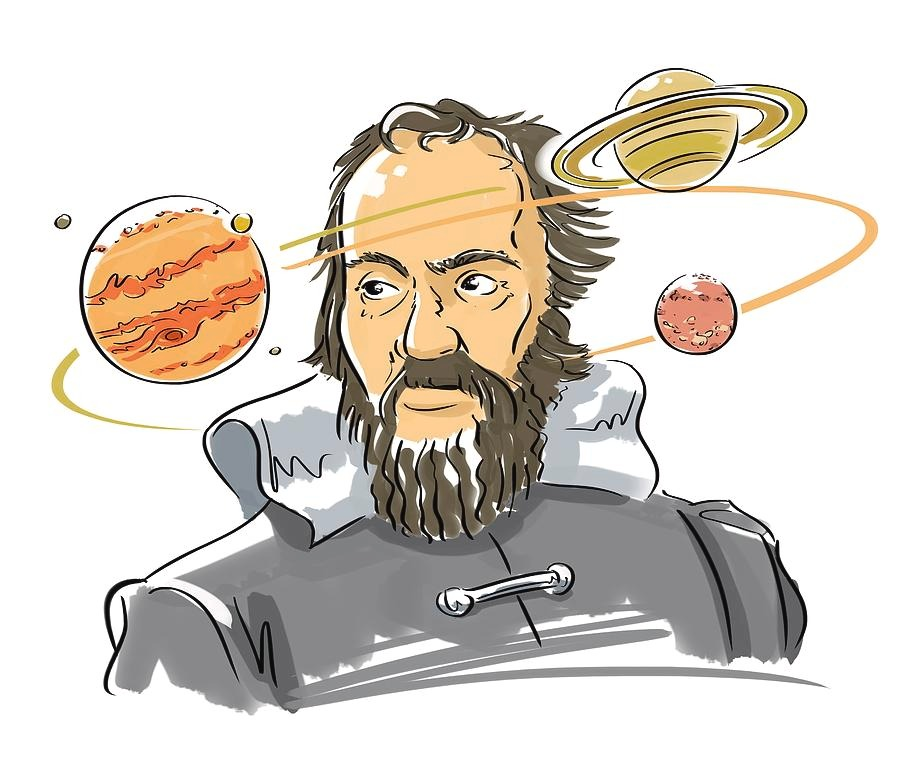
\includegraphics[scale=0.4]{Galileo.jpg}
\epigraph{"La verità riesce a imporsi solo nella misura in cui noi la imponiamo; la vittoria della ragione non può essere che la vittoria di coloro che ragionano."} {\textit{Vita di Galileo - Bertolt Brecht}}
}


\thispagestyle{empty}

\vspace*{0.4\textheight}

\begin{center}
  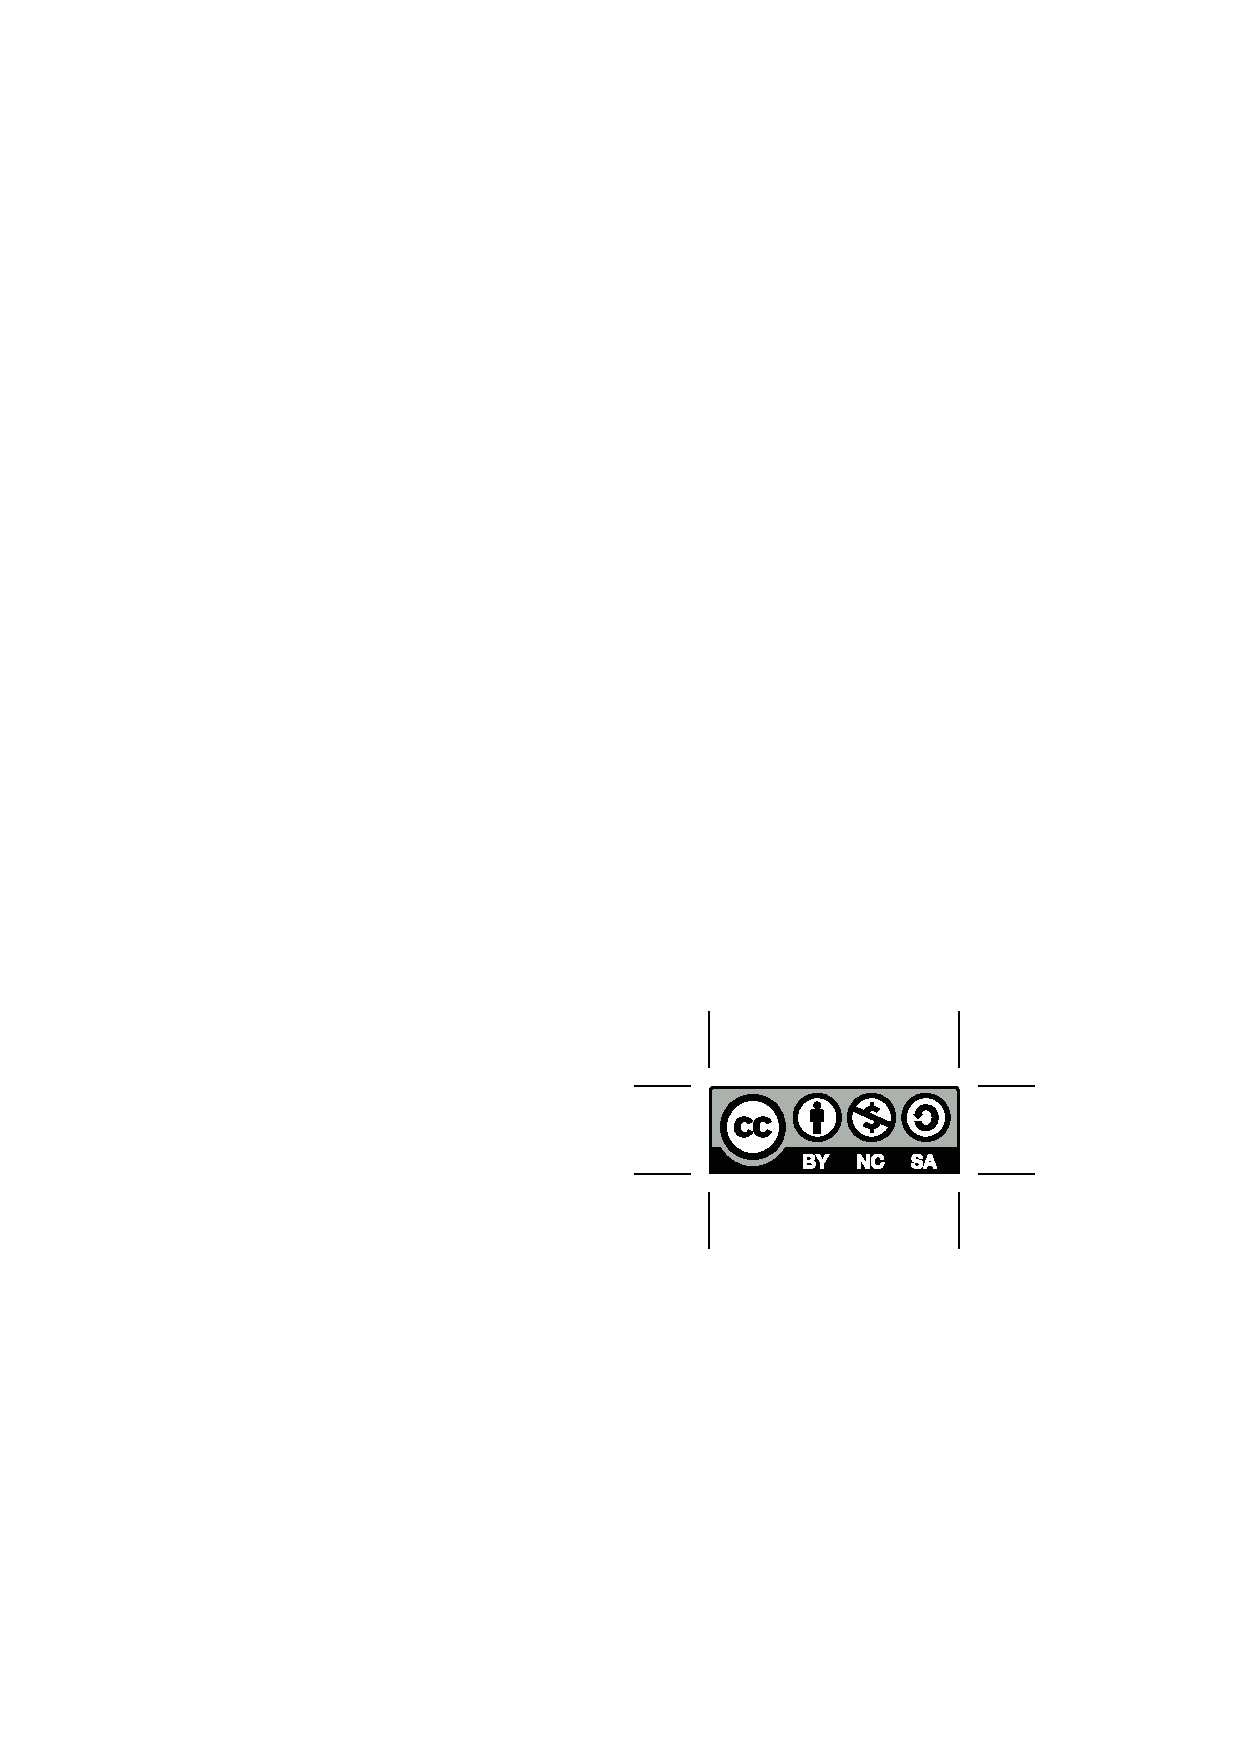
\includegraphics{misc/by-nc-sa}
\end{center}

\bigskip\noindent
This work is licensed under the Creative Commons Attribution-NonCommercial-ShareAlike 4.0 International License. To view a copy of this license, visit
\url{https://creativecommons.org/licenses/by-nc-sa/4.0/} or send a letter to
Creative Commons, PO Box 1866, Mountain View, CA 94042, USA.

\cleardoublepage


\chapter{Prefazione}
\section*{Guida alla consultazione}
\addcontentsline{toc}{section}{Guida alla consultazione}
La presente raccolta ha l'obiettivo di consentire al Lettore di prendere dimestichezza coi fondamenti teorici e pratici della Fisica di base e (quindi) di superare agevolmente l'Esame di Fisica Generale per Agraria o Enologia. Un consiglio: la Fisica NON si apprende facendo esercizi. Nella Fisica ogni definizione, ogni concetto, ogni formula ha un ruolo preciso e matematicamente ben definito all'interno di una teoria coerente, con la quale è necessario avere un minimo di confidenza per poter trarre profitto dagli esercizi. In altre parole: è senza dubbio preferibile prima studiare bene la teoria e poi cimentarsi con gli esercizi. Sicuramente questi risulteranno molto più facili se avrete già chiara la struttura logica della teoria.\\

La raccolta è suddivisa in Capitoli, ognuno dei quali riguarda un macro-argomento del programma di Fisica Generale. All'interno di ogni capitolo troverete degli Esercizi e dei Problemi. I primi sono quesiti di carattere molto semplice, che richiedono la sola applicazione di concetti e formule basilari, che dovrebbero essere stati  appresi a lezione e sul libro di testo. \'E quindi indispensabile saperli risolvere senza difficoltà se si vuole superare l'esame. I Problemi invece hanno una struttura più articolata e richiedono, oltre allo Studio, logica e talvolta un pizzico di intuito. Sono catalogati in base alla difficoltà: quelli una stella sono poco più complessi degli Esercizi e corrispondono a un più che sufficiente livello di conoscenza; quelli due e tre stelle corrispondono a livelli di conoscenza buoni o addirittura ottimi e dovrebbero permettere il superamento della prova finale senza incertezze. \\

All'inizio della raccolta troverete anche un piccolo prontuario su come si affronta un esercizio di Fisica. Pensiamo che potrebbe risultare utile, specialmente per coloro che non hanno mai avuto  occasione, alle Scuole Superiori, di svolgere da soli problemi di Fisica. \\

\textbf{Buono studio e buon lavoro}!

\textit{Per errori o suggerimenti scrivete a: \href{mailto:d.delsarto2@studenti.unipi.it}{d.delsarto2@studenti.unipi.it} e \href{mailto:guglami@gmail.com}{guglami@gmail.com}
}

\newpage

\section*{Come si risolve un esercizio di Fisica}
\addcontentsline{toc}{section}{Come si risolve un esercizio di Fisica}

Quello che segue è un riferimento su come si imposta un problema di Fisica. È importante rimarcare che questo è solo un \textit{aiuto} a chi si cimenta nella talvolta ardua fatica dello svolgere problemi.

Un consiglio generale è quello di cercare sempre di capire cosa si sta facendo e non procedere a caso "rigirando" le formule: se questo approccio può funzionare su esercizi più semplici vi garantiamo che fallirà in situazioni più complesse come quelle delle prove in itinere o delle prove scritte.

Ecco dunque alcuni consigli:

\begin{enumerate}
\item \textbf{Disegnate un grafico}: nel grafico cercate di includere tutte le quantità rilevanti allo svolgimento del problema (forze, masse, distanze...). Se per problemi semplici può sembrarvi tempo sprecato, un grafico fatto \textit{bene} sarà uno devi vostri migliori alleati in problemi più articolati.
\item \textbf{Scegliete il riferimento migliore}: la scelta del sistema di riferimento spetta a voi: siete liberi di posizionare l'origine dove volete e di utilizzare coordinate cartesiane o polari. Spesso una scelta saggia del sistema di riferimento semplifica molto i calcoli.
\item \textbf{Scrivete i dati e le incognite}: per chi è alle prime armi con il calcolo letterale è facile confondere gli elementi noti da quelle che sono le incognite richieste. Farsi uno specchietto a inizio problema aiuta a non confondersi e a non perdere tempo.
\item \textbf{Risolvete i problemi in modo letterale}: oltre all'innegabile vantaggio di aver risolto un numero infinito di problemi, lasciando i dati espressi tramite un parametro (ad esempio invece di inserire il valore dell'angolo si può scrivere $\theta$), si ha un procedimento più "pulito" ed eventualmente si possono sfruttare semplificazioni algebriche (ad es. $\sin^2\theta+\cos^2\theta=1$).
\item \textbf{Controllate i casi limite}: dove possibile è interessante verificare se la descrizione che abbiamo dato del problema funziona andando a osservare alcuni casi limite. Ad esempio quando si tratta di angoli è interessate vedere cosa succede quando valgono 0° o 90°: sono spesso casi più intuitivi e una rapida verifica.
\item \textbf{Controllate le unità di misura}: nello specchietto del punto 2 è importante annotare anche le unità di misura di ogni dato in nostro possesso e delle incognite. Ad esempio se come dato ho la lunghezza $a$ del lato di un triangolo so che la sua unità di misura in KMS sarà $[a]=	\text{m}$, questo mi è utile perché, ottenuta l'espressione che identifica l'incognita cercata, posso controllare velocemente se corrisponde all'unità di misura che mi aspetto e che ho annotato nello specchietto (ad esempio per una velocità mi aspetto delle dimensioni m/s). 
\item \textbf{Controllate che le vostre equazioni abbiano senso}: non si possono sommare mele e pere! Quindi non posso sommare quantità che hanno dimensioni diverse (ad esempio metri con kg). Allo stesso modo vettori devono essere sommati con altri vettori e nelle equazioni vettoriali dovrò avere vettori al membro sinistro uguagliati a vettori al membro destro.
\item \textbf{Controllate gli argomenti di alcune funzioni}: funzioni esponenziali ($a^x$), logaritmiche ($\log(x)$) e trigonometriche ($\sin(x)$, $\cos(x)$, $\tan(x)$, $\atan(x)$, ecc...) devono avere argomento \textit{adimensionale}. Se quando eseguite il controllo dimensionale l'argomento di tali funzioni non è adimensionale avete sbagliato qualcosa.
\end{enumerate}

\tableofcontents
\thispagestyle{empty}
\newpage

\mainmatter

\chapter{Calcolo Vettoriale}
\section{Esercizi}
\subsection*{Esercizio 1}
Un vettore $\vec{v}$ che giace su un piano cartesiano ha 
coordinate $v_x=5 \;$m e $v_y=12 \;$cm rispetto ai due versori ortogonali $\hat{x}$ e $\hat{y}$. Qual è il modulo (o intensità) del vettore? Esprimere il risultato in m e cm. Quanto vale il prodotto scalare $\vec{v} \cdot \vec{v}$? Qual è la relazione fra questi due risultati?
\subsubsection*{Soluzione}
Per definizione il modulo di un vettore $\vec{v}$ a due componenti è:
\begin{equation*}
|\vec{v}|=\sqrt{(v_x)^2+(v_y)^2}
\end{equation*}
Chiaramente $v_x$ e $v_y$ devono avere le stesse dimensioni 
affinché questo calcolo abbia senso. Quindi bisogna fare delle banali conversioni:
\begin{gather*}
v_x=5 \; \text{m}= 500 \; \text{cm}\\
v_x=0.012 \; \text{m}= 12 \; \text{cm}
\end{gather*}
Applicando la formula precedente si ottiene quindi:
\begin{equation*}
|\vec{v}|\simeq 5.0014 \; \text{m} =  500.14 \; \text{cm}
\end{equation*}
Il prodotto scalare fra $\vec{v}$ e se stesso è invece definito come:
\begin{equation*}
\vec{v} \cdot \vec{v}=v_x v_x + v_y v_y=(v_x)^2 + (v_y)^2 
\end{equation*}
e quindi $\vec{v} \cdot \vec{v}=|\vec{v}|^2$, per cui il suo valore si ottiene semplicemente calcolando il quadrato del modulo di $\vec{v}$.

\subsection*{Esercizio 2}
Su un piano cartesiano si considerino i due vettori $\vec{a}=(1,2)$ e $\vec{b}=(-2,1)$. Si disegnino $\vec{a}$ e $\vec{b}$ e se ne calcoli il prodotto scalare $\vec{a}\cdot \vec{b}$. Quanto vale l'angolo $\theta$ tra essi compreso? Calcolare anche $\vec{a}+\vec{b}$, $\vec{a}-\vec{b}$ e i loro moduli (intensità) $|\vec{a}+\vec{b}|$ e $|\vec{a}-\vec{b}|$.
\subsubsection*{Soluzione}
I vettori $\vec{a}$ e $\vec{b}$ sono rappresentati in Figura \ref{fig:vettori1}.


 \begin{figure}[!ht]
\centering
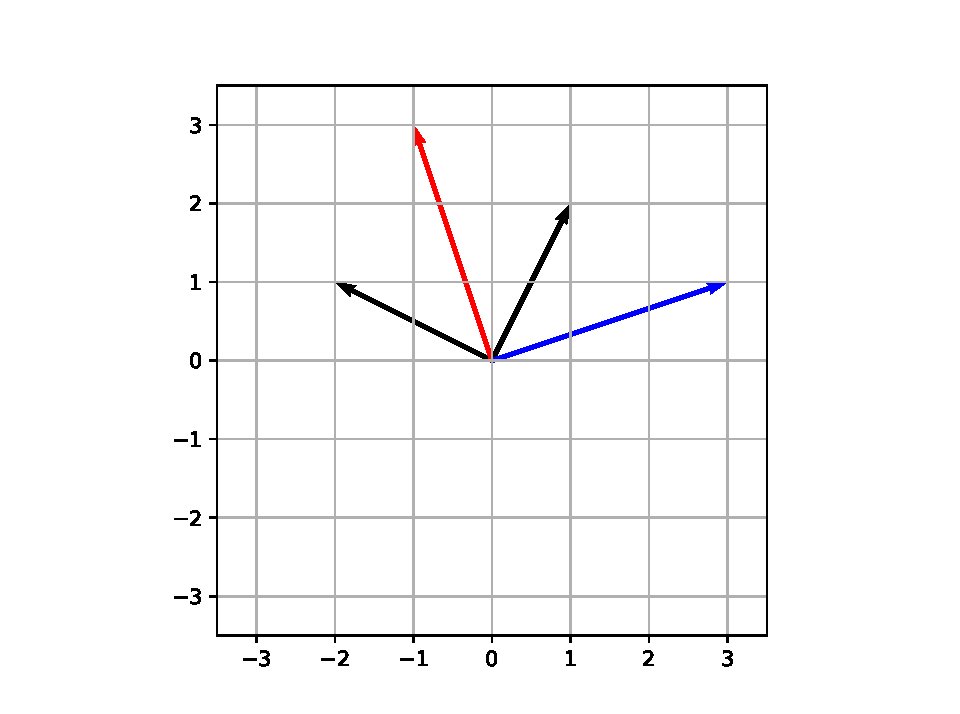
\includegraphics[scale=0.6]{vettori1.pdf}
\caption{Vettori $\vec{a}$ e $\vec{b}$ (in nero), $\vec{a}+\vec{b}$ (in rosso), $\vec{a}-\vec{b}$ (in blu) }
\label{fig:vettori1}
\end{figure}

(di colore nero).  Il prodotto scalare tra i due è:
\begin{equation*}
\vec{a} \cdot \vec{b}=a_x b_x + a_y b_y=-2+2=0
\end{equation*}
Come dovrebbe essere noto vale: $\vec{a} \cdot \vec{b}=|\vec{a}|| \vec{b}|\cos \theta$, dove $\theta$ è l'angolo compreso tra $\vec{a}$ e $\vec{b}$. Poiché  $\vec{a} \cdot \vec{b}=0$ e $|\vec{a}|>0$, $|\vec{b}|>0$, deve necessariamente valere: 
$\cos \theta=0$ e quindi $\theta=\frac{\pi}{2}=90^{\circ}$. In effetti come si vede dal disegno i due vettori sono perpendicolari!
I vettori $\vec{a}+\vec{b}$, $\vec{a}-\vec{b}$ si trovano semplicemente sommando o sottraendo le componenti di $\vec{a}$ e $\vec{b}$:
\begin{gather*}
\vec{a}+\vec{b}=\big(1+(-2), 2+1\big)=(-1,3)\\
\vec{a}-\vec{b}=\big(1-(-2), 2-1\big)=(3,1)
\end{gather*}
Questi due vettori sono rappresentati rispettivamente in rosso e in blu nella Figura \ref{fig:vettori1}. I loro moduli sono:
\begin{gather*}
|\vec{a}+\vec{b}|=\sqrt{(-1)^2+3^2}=\sqrt{10}\\
|\vec{a}-\vec{b}|=\sqrt{3^2+1^2}=\sqrt{10}
\end{gather*}

\subsection*{Esercizio 3}
Un vettore $\vec{v}$ ha modulo 2. Che modulo hanno i vettori $3\vec{v}$ e $-\vec{v}$? Quanto vale al più il modulo della somma di $-\vec{v}$ con un vettore $\vec{w}$ di modulo 3? Qual è l'angolo fra $\vec{v}$ e $\vec{w}$ in questo caso?
\subsubsection*{Soluzione}
Ovviamente $|3\vec{v}|=3|\vec{v}|$ e $|-\vec{v}|=|\vec{v}|$.In generale se $a$ è un numero (positivo o negativo):
\begin{gather*}
|a\vec{v}|=\sqrt{a^2 (v_x)^2+ a^2 (v_y)^2}=\sqrt{a^2} \sqrt{(v_x)^2+(v_y)^2}=|a||\vec{v}|
\end{gather*}
Per rispondere alla seconda domanda chiamiamo $\vec{w}$ il secondo vettore ($|\vec{w}|=3$) e $\theta$ l'angolo che questo forma con $\vec{v}$. Allora:
\begin{gather*}
|-\vec{v}+\vec{w}|^2=(-\vec{v}+\vec{w})\cdot (-\vec{v}+\vec{w})= \vec{v}\cdot \vec{v} + \vec{w}\cdot \vec{w} - 2 \vec{v}\cdot \vec{w}=\\
=|\vec{w}|^2 + |\vec{v}|^2 - 2|\vec{w}||\vec{v}|\cos \theta= 9 + 4 - 12\cos \theta=13-12\cos \theta
\end{gather*}
Quindi il modulo della somma di $-\vec{v}$ con $\vec{w}$ è massimo quando $\cos \theta=-1$, ovvero $\theta=\pi=180^{\circ}$. In questo si ha:
\begin{gather*}
|-\vec{v}+\vec{w}|^2=13+12=25 \quad \Rightarrow \quad |-\vec{v}+\vec{w}|=5
\end{gather*}
come del resto era intuitivo ($-\vec{v}$ e $\vec{w}$ hanno stessa direzione e stesso verso, quindi i moduli si sommano).


\subsection*{Esercizio 4}
Un vettore $\vec{v}$ ha modulo 1 e forma un angolo di 30$^{\circ}$ gradi rispetto al versore $\hat{x}$ di un piano cartesiano. Inoltre si sa che la componente $v_y$ è positiva. Si calcolino i valori esatti delle due componenti di $\vec{v}$. 
\subsubsection*{Soluzione}
Il vettore $\vec{v}$ ha modulo $1$, quindi appartiene alla circonferenza goniometrica. Detto $\theta=$30$^{\circ}$ l'angolo compreso tra 
$\vec{v}$ e $\hat{x}$, si ha allora:
\begin{gather*}
v_x=\cos \theta\\
v_y=\sin \theta
\end{gather*}
dove si è utilizzata l'informazione $v_y>0$ per prendere il vettore con $v_y=+\sin \theta$ anziché quello con $v_y=-\sin \theta$. Ricordando i valori 
di $\sin 30^{\circ}$ e $\cos 30^{\circ}$, si ottiene subito: $\vec{v}=(\frac{\sqrt{3}}{2}, \frac{1}{2})$. 

\subsection*{Esercizio 5}
Un uomo si muove lungo le vie della sua città. La mappa della città è un piano cartesiano con coordinate $(x,y)$ e origine O coincide col punto di partenza dell'uomo $(x_i, y_i)$. L'uomo effettua tre spostamenti consecutivi rappresentati sulla mappa dai vettori: $\vec{\Delta r_1}=(1,1)$ $\vec{\Delta r_2}=(-1,2)$ e $\vec{\Delta r_3}=(5/2,-3/2)$. Quali sono le coordinate $(x_f, y_f)$ del punto di arrivo dell'uomo? Quanta distanza $d$ ha percorso? Quanta distanza $d'$ deve ancora percorrere \textit{al minimo} se vuole tornare al punto di partenza? Ricordiamo che il vettore spostamento relativo a una traiettoria che parte da $(x_i, y_i)$ e termina in $(x_f,y_f)$ è $\vec{\Delta r}=(x_i-x_f, y_i-y_f)$. 
\subsubsection*{Soluzione}
Conviene partire da un disegno sul piano cartesiano dei tre vettori spostamento. Per farlo si devono disegnare uno di seguito all'altro $\vec{\Delta r_1}, \vec{\Delta r_2}, \vec{\Delta r_3}$. Il risultato sono i tre vettori in nero in Figura \ref{fig:vettori2}.

 \begin{figure}[!ht]
\centering
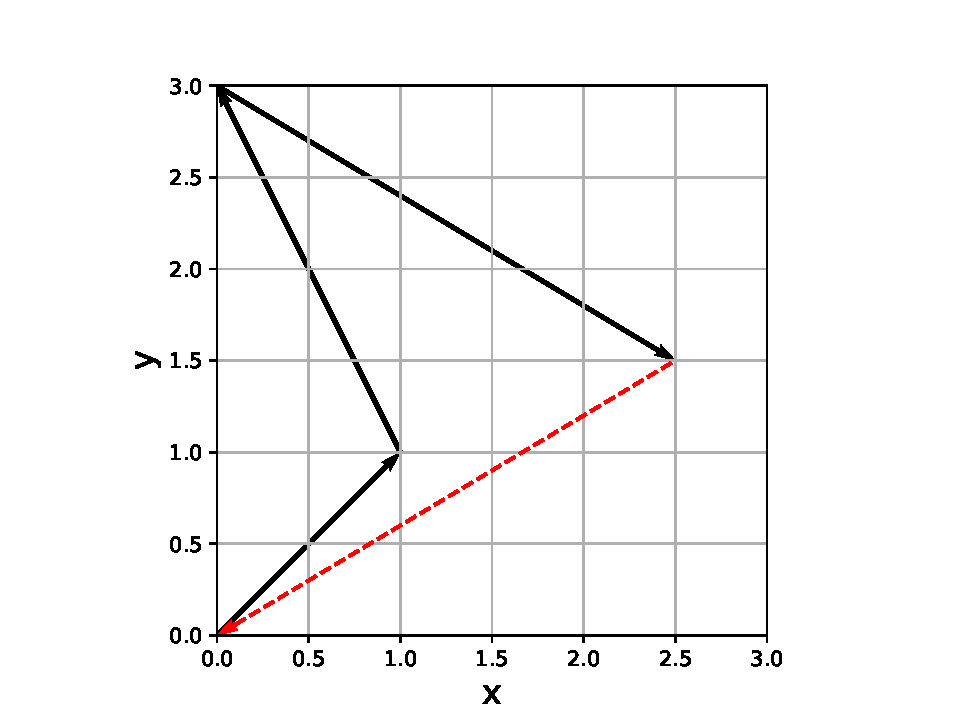
\includegraphics[scale=0.6]{vettori2.pdf}
\caption{I tre vettori spostamento $\vec{\Delta r_1}, \vec{\Delta r_2}, \vec{\Delta r_3}$ (in nero), e il vettore $\vec{\Delta r_4}$ necessario per tornare al punto di partenza percorrendo la minima distanza (in rosso, tratteggiato).  }
\label{fig:vettori2}
\end{figure}

Le coordinate del punto di arrivo si ottengono subito dal disegno o, in modo equivalente, sommando $\vec{\Delta r_1}, \vec{\Delta r_2}, \vec{\Delta r_3}$ alle coordinate del punto di partenza:
\begin{gather*}
x_f=x_i +1 + (-1) +5/2= 0 + 5/2=5/2\\
y_f=y_i +1 + 2 - 3/2= 3 - 3/2=3/2
\end{gather*}
Quindi il punto di arrivo è $(5/2, 3/2)$. La distanza percorsa si trova sommando i moduli dei singoli vettori spostamenti. Si ha:
\begin{gather*}
|\vec{\Delta r_1}|=\sqrt{2} \\
|\vec{\Delta r_2}|=\sqrt{5} \\
|\vec{\Delta r_3}|=\frac{\sqrt{34}}{2}
\end{gather*}
per cui la distanza percorsa è: $d=\sqrt{2}+\sqrt{5}+\frac{\sqrt{34}}{2}$. La distanza che rimane da percorrere (al minimo) corrisponde al modulo 
del vettore posizione finale (si veda \ref{fig:vettori2}). Quindi:
\begin{gather*}
d'=\sqrt{(5/2)^2+(3/2)^2}=\frac{\sqrt{34}}{2}
\end{gather*}

\subsection*{Esercizio 6}
Dati due vettori generici $\vec{v}=(v_x, v_y)$ e $\vec{w}=(w_x, w_y)$ sul piano cartesiano esprimere le coordinate della loro somma e trovare il suo modulo in funzione dei valori di $v_x, v_y, w_x, w_y$. Può essere negativo tale modulo? Può valere 0? In quali casi? 
\subsubsection*{Soluzione}
La somma dei due vettori ha come coordinate cartesiane la somma delle cordinate di $\vec{v}$ e $\vec{w}$, quindi:
\begin{gather*}
\vec{v}+\vec{w}=(v_x+w_x, v_y+w_y)
\end{gather*}
Il suo modulo è per definizione:
\begin{gather*}
|\vec{v}+\vec{w}|=\sqrt{(v_x+w_x)^2 + (v_y+w_y)^2}
\end{gather*}
Ovviamente il modulo di un vettore NON può MAI essere negativo (infatti si ottiene facendo una radice quadrata!). Può invece valere $0$. Poiché nell'espressione precedente vi sono due quadrati (che sono sempre $\geq0$), devono essere entrambi $=0$ se la radice quadrata deve fare $0$. Quindi affinché $|\vec{v}+\vec{w}|=0$ si deve avere:
\begin{gather*}
v_x+w_x=0 \quad \Rightarrow \quad w_x=-v_x \\
v_y+w_y=0 \quad \Rightarrow \quad w_y=-v_y
\end{gather*}
cioè i due vettori devono essere opposti. 

\subsection*{Esercizio 7}
Dato il vettore $\vec{a}=(\sqrt{2}/2, \sqrt{2}/2)$ si dica come deve essere fatto un secondo vettore $\vec{b}$ in modo che $\vec{a}-\vec{b}$ sia parallelo all'asse y. Nel caso in cui $\vec{b}$ abbia modulo 2 e $b_y$ sia positivo, si scrivano esplicitamente le sue componenti. Si calcoli inoltre il vettore $\vec{a}+\vec{b}$ e si l'angolo che esso forma con l'asse x. 
\subsubsection*{Soluzione}
Sia in generale $\vec{b}=(b_x, b_y)$. Si ha:
\begin{gather*}
\vec{a}-\vec{b}=(\sqrt{2}/2-b_x, \sqrt{2}/2-b_y)
\end{gather*}
Un vettore è parallelo all'asse $y$ quando ha la prima componente $=0$ e la seconda $\neq 0$. Quindi affinché si abbia $\vec{a}-\vec{b}$ parallelo all'asse y  , si deve avere $b_x=\sqrt{2}/2$ e $b_y \neq \sqrt{2}/2$. Imponiamo ora che il modulo di $\vec{b}$ sia $2$:
\begin{gather*}
|\vec{b}|=\sqrt{(\sqrt{2}/2)^2 + (b_y)^2}=\sqrt{\frac{1}{2} + (b_y)^2}=2  \quad \Rightarrow \quad (b_y)^2=4-\frac{1}{2}=\frac{7}{2}
\end{gather*}
e quindi: $b_y=\frac{\sqrt{7}}{\sqrt{2}}$ (c'era anche la soluzione  $b_y=-\frac{\sqrt{7}}{\sqrt{2}}$ ma l'abbiamo scartata perché nel testo si dice esplicitamente che $b_y>0$).
In definitiva:
\begin{gather*}
\vec{b}=(\frac{\sqrt{2}}{2}, \frac{\sqrt{7}}{\sqrt{2}})
\end{gather*}
Il vettore $\vec{a}+\vec{b}$ sarà:
\begin{gather*}
\vec{a}+\vec{b}=(\frac{\sqrt{2}}{2}+\frac{\sqrt{2}}{2}, \frac{\sqrt{2}}{2}+\frac{\sqrt{7}}{\sqrt{2}})= (\sqrt{2}, \frac{1+\sqrt{7}}{\sqrt{2}}) \simeq (1.414, 2.578)
\end{gather*}
L'angolo $\theta$ che esso forma con l'asse $x$ si trova facendo il prodotto scalare $(\vec{a}+\vec{b})\cdot \hat{x}=|\vec{a}+\vec{b}|\cos \theta$. Si ha: 
\begin{gather*}
(\vec{a}+\vec{b})\cdot \hat{x}=\sqrt{2}
\end{gather*}
e inoltre:
\begin{gather*}
|\vec{a}+\vec{b}|=\sqrt{2+\frac{1}{2}(1+\sqrt{7})^2}=\sqrt{2+\frac{1}{2}(8+2\sqrt{7})}=\sqrt{6+\sqrt{7}}
\end{gather*}
per cui:
\begin{gather*}
\cos \theta=\frac{(\vec{a}+\vec{b})\cdot \hat{x}}{|\vec{a}+\vec{b}|}=\frac{\sqrt{2}}{\sqrt{6+\sqrt{7}}} \simeq 0.481
\end{gather*}
e infine $\theta\simeq 1.069 \; \text{rad} \simeq 61^{\circ}$.


\subsection*{Esercizio 8}
Un vettore tridimensionale $\vec{v}=(v_x, v_y, v_z)$ ha componenti $v_y= 1\;$m e $v_z=7\;$cm. Sapendo che il modulo del vettore è $|v|=100.846\;$cm si dica quanto vale la componente $v_x$, in cm e m. Si calcoli inoltre il prodotto scalare di $\vec{v}$ con il vettore $\vec{w}=(0,0,1)\;$m, determinando poi l'angolo compreso tra i due.

\subsubsection*{Soluzione}
Si ha $v_y=10^2\;$ cm e quindi
\begin{gather*}
|\vec{v}|^2=(v_x)^2+(v_y)^2+(v_z)^2=(v_x)^2+10000 \; \text{cm}^2 + 49 \; \text{cm}^2=(100.846)^2  \; \text{cm}^2 \simeq 10170\; \text{cm}^2
\end{gather*}
da cui si ricava: 
\begin{gather*}
(v_x)^2 \simeq 121\; \text{cm}^2 \quad \Rightarrow \quad v_x=\pm 11\; \text{cm} 
\end{gather*}
o anche $v_x =\pm 0.11 \;$m. Entrambe le soluzioni sono accettabili. Bisogna poi calcolare il prodotto scalare $\vec{v}\cdot \vec{w}$, con $\vec{w}=(0,0,1)\;$m che dà come risultato:
\begin{gather*}
\vec{v}\cdot \vec{w}=7 \cdot 10^{-2} \; \text{m}^2
\end{gather*}
Dato che $\vec{v}\cdot \vec{w}=|\vec{v}||\vec{w}| \cos \theta$, dove $\theta$ è l'angolo compreso tra i due vettori, si ha:
\begin{gather*}
\cos \theta=\frac{\vec{v}\cdot \vec{w}}{|\vec{v}||\vec{w}|}=\frac{7 \cdot 10^{-2} \; \text{m}^2}{1.00846 \; \text{m}^2}\simeq 0.0694
\end{gather*}
da cui: 
\begin{gather*}
\theta \simeq \text{arcos}(0.0694) \simeq 1.501 \; \text{rad} \simeq 86^{\circ}
\end{gather*}

\subsection*{Esercizio 9}
Sia dato un vettore $\vec{v}$ di modulo $90\;\text{m}$ e componente $v_x=-70\;\text{m}$. Quali sono i possibili valori per la componente $v_y$. Assumendo $v_y$ positiva, trovare il vettore $\vec{q}$ che, sommato a quello di partenza, dia un vettore risultante $\vec{w}$ di modulo $120\;\text{m}$ e parallelo all'asse $x$ con verso negativo.

\subsubsection*{Soluzione}
Dobbiamo risolvere la seguente equazione:
%
\begin{equation*}
\qty|\vec{v}|=\sqrt{v_x^2+v_y^2}
\end{equation*}
%
Possiamo elevare entrambi i membri al quadrato in quanto il modulo di un vettore $\qty|\vec{v}|$ è sempre una quantità positiva:
%
\begin{equation*}
\qty|\vec{v}|^2=v_x^2+v_y^2
\end{equation*}
%
Risolviamo l'equazione per $v_y$ ed inseriamo i valori numerici del testo:
%
\begin{gather*}
v_y=\pm\sqrt{\qty|\vec{v}|^2-v_x^2}=\pm\sqrt{(90\;\text{m})^2-(-70\;\text{m})^2}=\pm40\sqrt{2}\;\text{m}\approx \pm 56.6\;\text{m}
\end{gather*} 
%
Adesso consideriamo, come indicato dall'esercizio, il risultato positivo e cerchiamo il vettore $\vec{w}$ che sappiamo essere parallelo all'asse $x$, quindi $w_y=0$, e con verso negativo $w_x<0$.
%
\begin{equation*}
\qty|\vec{w}|=w_x=\pm 120\;\text{m} \Rightarrow w_x=-120\;\text{m}
\end{equation*}
%
Imponiamo dunque la condizione sulla somma e risolviamo per componenti:
%
\begin{gather*}
\vec{w}=\vec{v}+\vec{q} \\
w_x\hat{x} = (v_x+q_x)\hat{x} + (v_y+q_y)\hat{y}
\end{gather*} 
%
Uguagliando le componenti corrispondenti per i due membri delle equazioni si ottiene immediatamente: 
%
\[
\begin{cases}
	w_x=v_x+q_x \Rightarrow q_x=w_x-v_x= -120\;\text{m} + 70\;\text{m}=-50\;\text{m} \\
    0=v_y+q_y \Rightarrow q_y=-v_y \approx - 56.6\;\text{m}
\end{cases}
\]
%

\section{Problemi}

\subsection{Operazioni basilari fra vettori \rstar}
Sono definiti due vettori:
%
\begin{equation*}
\vec{a}=(4\;\text{m})\hat{x}-(3\;\text{m})\hat{y} \qquad \qquad \vec{b}=(3\;\text{m})\hat{x}+(7\;\text{m})\hat{y}
\end{equation*}
%
Calcolare il modulo e l'angolo (relativo all'asse $x$) di $\vec{a}$, $\vec{b}$, $\vec{a}+\vec{b}$, $\vec{a}-\vec{b}$, $\vec{b}-\vec{a}$. Quale è l'angolo fra la direzione di $\vec{a}+\vec{b}$ e $\vec{a}-\vec{b}$? E fra $\vec{b}-\vec{a}$ e $\vec{a}-\vec{b}$?

\subsubsection*{Soluzione}
Per ciascuna richiesta ragioniamo per componenti, ricordiamo che l'angolo che forma un vettore $\vec{v}$ con l'asse $x$ è dato da $\tan\theta=v_y/v_x$. Abbiamo allora:
%
\begin{gather*}
\qty|\vec{a}|=\sqrt{(4^2+(-3)^2)\;\text{m}^2}=5\;\text{m} \qquad \tan\theta=-\frac{3\;\text{m}}{4\;\text{m}} \Rightarrow \theta=\arctan\qty(-\frac{3\;\text{m}}{4\;\text{m}})\approx-36.9\degree \\
\qty|\vec{b}|=\sqrt{(3^2+7^2)\;\text{m}^2}\approx 7.6\;\text{m} \qquad \tan\theta=\frac{7\;\text{m}}{3\;\text{m}} \Rightarrow \theta=\arctan\qty(\frac{7\;\text{m}}{3\;\text{m}})\approx66.8\degree \\
\qty|\vec{a}+\vec{b}|=\sqrt{((4+3)^2+(-3+7)^2)\;\text{m}^2}\approx 8.1\;\text{m} \qquad \tan\theta=\frac{4\;\text{m}}{7\;\text{m}} \Rightarrow \theta=\arctan\qty(\frac{4\;\text{m}}{7\;\text{m}})\approx 29.7\degree \\
\qty|\vec{a}-\vec{b}|=\sqrt{((4-3)^2+(-3-7)^2)\;\text{m}^2}\approx 10.0\;\text{m} \qquad \tan\theta=-\frac{10\;\text{m}}{1\;\text{m}} \Rightarrow \theta=\arctan\qty(-\frac{10\;\text{m}}{1\;\text{m}})\approx -84.3\degree 
\end{gather*}
%
Per calcolare l'angolo fra le direzioni di $\vec{a}+\vec{b}$ e $\vec{a}-\vec{b}$ basta prendere il valore assoluto della differenza dei due angoli che formano con l'asse $x$ ovvero: $\qty|29.7\degree-(-84.3\degree)|\approx 114\degree$.\\

Notiamo adesso che $\vec{a}-\vec{b}=(-1)(\vec{b}-\vec{a})$, ovvero sono vettori che hanno lo stesso modulo, $\qty|\vec{a}-\vec{b}|=\qty|(-1)(\vec{b}-\vec{a})|= \qty|(\vec{b}-\vec{a})|$, ma verso opposto, quindi non c'è bisogno di eseguire alcun calcolo aggiuntivo. Per queste considerazioni l'angolo fra le loro direzioni è 0. In Figura \ref{fig:vec_op} i vettori e le risultanti con la costruzione geometrica.

\begin{figure}[h]
 \centering
\scalebox{1.5}[1.2]
	{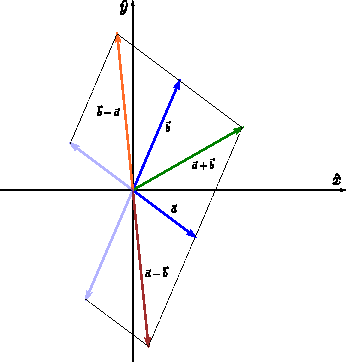
\includegraphics{vec_op.pdf}}
 \caption{Vettori base e risultanti, i vettori semitrasparenti sono i vettori opposti a quelli dati.}
 \label{fig:vec_op}
\end{figure}

\pagebreak

\subsection{Componenti di $g$ su piano inclinato \rstar}
\label{subsec:incline}
Un piano è inclinato di un angolo di $\vartheta$ rispetto all'orizzontale. Sul piano si scelga l'asse $x'$ nella direzione di massima pendenza verso il basso e si prenda invece l'asse $y'$ perpendicolare al piano nel verso che si allontana dal piano. Si trovino le componenti $x'$ e $y'$ dell'accelerazione di gravità, che ha modulo $9.8\;\text{m/s}^2$ ed è diretta verticalmente verso il basso. Risolvere numericamente per $\vartheta = 30$°
\subsubsection*{Soluzione}

\begin{figure}[h]
 \centering
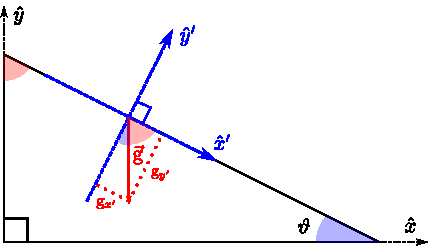
\includegraphics[scale=1.3]{drawing.pdf}
 \caption{Schema del problema con riferimento obliquo}
 \label{figure:incline_g}
\end{figure}

Per la soluzione dell'esercizio serviranno alcuni ragionamenti geometrici: l'angolo al vertice (rosso in figura) è congruente con l'angolo che la direzione di $\vec{g}$ forma con il versore $\hat{x'}$ perché angoli corrispondenti di due rette parallele tagliate da una trasversale; conseguentemente, per differenza con l'angolo retto, potremo identificare $\vartheta$ con l'angolo che la direzione di $\vec{g}$ forma con il versore $-\hat{y'}$. Adesso siamo in grado di ricavare le componenti nel sistema di riferimento obliquo grazie ai prodotti scalari con i versori direttori:
%
\begin{gather*}
g_{y'}= \vec{g}\cdot (-)\hat{y}'=-g\cos(\vartheta) \\
g_{x'}= \vec{g}\cdot \hat{x}'=g\cos(\pi/2 - \vartheta)=g\sin(\vartheta) \\
\end{gather*} 
%
Che, con i valori numerici del testo diventano:
%
\begin{gather*}
-g\cos(\vartheta) = -9.8 \cdot \frac{\sqrt{3}}{2}\;\text{m/s}^2=-4.9\;\text{m/s}^2 \\
g\sin(\vartheta) = 9.8 \cdot \frac{1}{2}\;\text{m/s}^2 \approx 8.49\;\text{m/s}^2 \\
\end{gather*} 
%
\textit{Meno geometria... più fisica}: fermo restando che è un approccio da prendere con le dovute precauzioni, nel controllare se i nostri ragionamenti geometrici sono esatti si possono analizzare le situazioni agli estremi di definizione del parametro, in questo caso $\vartheta$. \\
Poniamo infatti di scegliere $\vartheta=0$, in questo caso avremo i versori $\hat{y}$ e $\hat{y}'$ paralleli e quindi $g_y=g_{y'}=-g$, massima in valore assoluto, mentre la componente orizzontale sarà 0, questo conferma l'andamento da noi previsto della componente $g_{y'}\propto - \cos(\vartheta)$: infatti il coseno è massimo per $\vartheta=0$. Ragionamento analogo si può fare per la componente $\hat{x}'$.


\subsection{Vettori nello spazio \rstar}
Dati tre vettori nello spazio:
\begin{equation*}
\vec{a}=(4\;\text{m})\hat{x}+(5\;\text{m})\hat{y}+(6\;\text{m})\hat{z} \qquad \vec{b}=(3\;\text{m})\hat{x}+(3\;\text{m})\hat{y}+(2\;\text{m})\hat{z} \qquad \vec{c}=(2\;\text{m})\hat{x}+(5\;\text{m})\hat{y}+(3\;\text{m})\hat{z}
\end{equation*}

Definiamo $\vec{r}=\vec{a}+\vec{b}-\vec{c}$, trovarne il modulo e calcolare l'angolo fra $\vec{r}$ e la direzione positiva dell'asse $z$. Qual è la componente di $\vec{b}$ lungo la direzione di $\vec{c}$?

\subsubsection*{Soluzione}
Procediamo con una normale somma per componenti in modo da trovare il modulo di $\vec{r}$:
%
\begin{gather*}
\vec{r}=(a_x+b_x-c_x)\hat{x}+(a_y+b_y-c_y)\hat{y}+(a_z+b_z-c_z)\hat{z}=(5\;\text{m})\hat{x}+(3\;\text{m})\hat{y}+(5\;\text{m})\hat{z}\\
\qty|\vec{r}|=\sqrt{(5\;\text{m})^2+(3\;\text{m})^2+(5\;\text{m})^2}\approx 7.7\;\text{m}
\end{gather*} 
%
Per trovare l'angolo che $\vec{r}$ forma con l'asse $z$ basta farne il prodotto scalare con il versore direttore $\hat{z}$. A tal proposito è necessario ricordare la definizione del prodotto scalare per moduli e per componenti ed inoltre che i versori direttori sono perpendicolari fra loro ($\hat{x}\cdot\hat{y}=\hat{x}\cdot\hat{z}=\hat{y}\cdot\hat{z}=0$)
%
\begin{gather*}
\vec{r}\cdot\hat{z}=r_z=\qty|\vec{r}|\cos\theta \\
\cos\theta=\frac{r_z}{r} \Rightarrow \theta=\arccos\qty(\frac{r_z}{r})\approx 49.5\degree
\end{gather*} 
%
Volendo trovare la componente di $\vec{b}$ lungo la direzione di $\vec{c}$   la via più breve è trovare il versore direttore di $\vec{c}$ (NB, questo \textit{non} è ortogonale con gli altri vettori direttori in quanto non è uno di quelli di base del sistema rettangolare cartesiano), ricaviamo il versore $\hat{c}$ in funzione dei versori di base rettangolari:
%
\begin{gather*}
\hat{c}=\frac{\vec{c}}{\qty|c|}=\frac{(2\;\text{m})\hat{x}+(5\;\text{m})\hat{y}+(3\;\text{m})\hat{z}}{\sqrt{(2\;\text{m})^2+(5\;\text{m})^2+(3\;\text{m})^2}}=\frac{(2\;\text{m})\hat{x}+(5\;\text{m})\hat{y}+(3\;\text{m})\hat{z}}{\sqrt{38}}
\end{gather*} 
%
Adesso ci basterà proiettare $\vec{b}$ lungo questa direzione, ovvero fare il prodotto scalare con il versore direttore: 
%
\begin{equation*}
b_c= \vec{b}\cdot\hat{c}=b_xc_x+b_yc_y+b_zc_z
\end{equation*} 
%
Sostituiamo infine i valori numerici relativi alle componenti in esame
%
\begin{equation*}
b_c=\qty(\frac{3\sqrt{38}}{19}+\frac{15\sqrt{38}}{38}+\frac{3\sqrt{38}}{19})\;\text{m}=\frac{27\sqrt{38}}{38}\;\text{m}\approx 4.4\;\text{m}
\end{equation*} 
%

\subsection{Coordinate Polari $\spadesuit$}
\label{subsec:polar}
Un sistema di riferimento alternativo, ma altrettanto utile, è quello che identifica un punto nel piano data la sua distanza dal centro e il suo angolo rispetto all'asse $x$; sistemi di riferimenti come questo sono chiamati \textit{polari}. I versori di questo sistema di riferimento sono due: uno diretto dall'origine verso il punto, l'altro perpendicolare ad esso; sono rispettivamente chiamati versore \textit{radiale} $\hat{r}$ e versore \textit{tangenziale} $\hat{\phi}$.\\
Il termine tangenziale deriva dal poter sempre individuare una circonferenza che abbia per centro l'origine, di raggio la distanza punto origine e che ovviamente contenga il punto; si traccia quindi la tangente e si individua un vettore unitario rivolto con verso pari a quello di crescita dell'angolo polare (antiorario).\\
La grande differenza con i versori cartesiani è che in generale i versori polari sono funzioni del tempo, quindi $\hat{r}(t)$ e $\hat{\phi}(t)$, un'osservazione che si rivelerà importante nel caso si facciano derivate.
La situazione descritta è riassunta in Figura \ref{fig:polar}. Vogliamo trovare le trasformazioni che ci permettano di passare dal riferimento polare a quello cartesiano e viceversa.

\begin{figure}[h]
 \centering
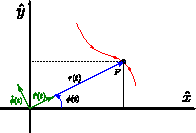
\includegraphics[scale=2.3]{polar.pdf}
 \caption{Traiettoria di un punto, componenti polari e versori polari (verdi).}
 \label{fig:polar}
\end{figure}

\subsubsection*{Soluzione}
Ipotizziamo di osservare un punto fermo, quindi facciamo cadere la dipendenza dal tempo nel procedimento che segue (non si perde di generalità).\\

\textbf{Polare $\rightarrow$ Cartesiano}: L'idea fondamentale è quella di prendere un generico vettore $\vec{v}$ definito in coordinate polari e di proiettarlo lungo i versori direttori cartesiani:
%
\begin{gather*}
\vec{v}=v_r\hat{r}+v_\phi\hat{\phi}\\
v_x=\vec{v}\cdot\hat{x}=v_r\hat{r}\cdot\hat{x}+v_\phi\hat{\phi}\cdot\hat{x} \qquad v_y=\vec{v}\cdot\hat{y}=v_r\hat{r}\cdot\hat{x}+v_\phi\hat{\phi}\cdot\hat{y}
\end{gather*} 
%
Si può facilmente ricavare tramite la trigonometria che $\hat{r}\cdot\hat{x}=\cos\phi$ e $\hat{r}\cdot\hat{y}=\sin\phi$, per i prodotti scalari con il versore tangente si ha $\hat{\phi}\cdot\hat{x}=\cos(\phi+\pi/2)=-\sin\phi$ e $\hat{\phi}\cdot\hat{y}=\cos\phi$. Otteniamo dunque:
%
\begin{gather*}
v_x=v_r\cos\phi-v_\phi\sin\phi \qquad v_y=v_r\sin\phi+v_\phi\cos\phi
\end{gather*} 
%
Ricaviamo quindi le trasformazioni dei versori dividendo per il modulo $\qty|\vec{v}|$ (uguale qualunque sia il sistema di riferimento) entrambi i membri:
%
\begin{gather*}
\hat{x}=\cos\phi\hat{r}-\sin\phi\hat{\phi} \qquad \hat{y}=\sin\phi\hat{r}+\cos\phi\hat{\phi}
\end{gather*} 
%
Si può risolvere per $\hat{r}$ e $\hat{\phi}$ ottenendo:
%
\begin{gather*}
\hat{r}=\cos\phi\hat{x}+\sin\phi\hat{y} \qquad \hat{\phi}=-\sin\phi\hat{x}+\cos\phi\hat{y}
\end{gather*} 
%
Infine scriviamo le relazioni che legano le quantità cartesiane con quelle polari:
%
\begin{gather*}
x=r\cos\phi \qquad \qquad y=r\sin\phi
\end{gather*} 
%
\\
\textbf{Cartesiano $\rightarrow$ Polare:} Abbiamo già ottenuto nella parte precedente le equazioni che legano i versori dei due sistemi di riferimento, supponiamo di avere un generico vettore in coordinate cartesiane $\vec{v}=v_x\hat{x}+v_y\hat{y}$, sostituendo i versori con quelli polari si otterrà:
%
\begin{gather*}
\vec{v}=v_x(\cos\phi\hat{r}-\sin\phi\hat{\phi})+v_y(\sin\phi\hat{r}+\cos\phi\hat{\phi}) \\
v_r=v_x\cos\phi+v_y\sin\phi \qquad v_\phi=-v_x\sin\phi+v_y\cos\phi
\end{gather*} 
%
Le relazioni che legano le quantità polari a quelle cartesiane sono:
%
\begin{gather*}
r=\sqrt{x^2+y^2} \qquad \qquad \tan\phi=\frac{y}{x}
\end{gather*} 
%
Quindi nel caso volessimo scrivere le relazioni precedenti solo utilizzando quantità cartesiane avremo:
%
\begin{gather*}
v_r=v_x\frac{x}{\sqrt{x^2+y^2}}+v_y\frac{y}{\sqrt{x^2+y^2}} \qquad v_\phi=-v_x\frac{y}{\sqrt{x^2+y^2}}+v_y\frac{x}{\sqrt{x^2+y^2}}
\end{gather*} 
%

\subsection{Angolo fra vettori di stesso modulo \rstar\rstar}
Due vettori $\vec{a}$ e $\vec{b}$ hanno lo stesso modulo $a$. Se la somma di questi due vettori vale $\vec{c}=c_x\hat{x}$, determinare l'angolo fra $\vec{a}$ e $\vec{b}$. Risolvere per $a=5\;\text{m}$ e $c_x=\sqrt{2}\cdot\;\text{m}$, con questi valori sapreste dare una risposta per via geometrica?

\subsubsection*{Soluzione}
Sapendo che i vettori hanno lo stesso modulo e la risultante non ha componente verticale è facile dedurre che le componenti verticali dei due vettori si devono annullare e che quindi siano l'uno il simmetrico dell'altro rispetto all'asse $x$, quindi anche l'angolo che formano con tale asse sarà lo stesso. Si veda Figura \ref{fig:vec_ang} per riferimento.

\begin{figure}[h]
 \centering
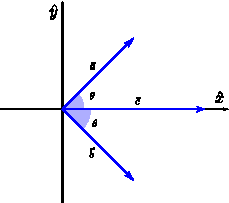
\includegraphics[scale=2.0]{vec_ang.pdf}
 \caption{Schematizzazione dei vettori in gioco}
 \label{fig:vec_ang}
\end{figure}

Vediamo la cosa matematicamente così da ottenere il valore dell'angolo, iniziamo scrivendo la somma per componenti:
%
\begin{gather*}
\vec{c}=\vec{a}+\vec{b}\\
c_x\hat{x}=(a_x+b_x)\hat{x}+(a_y+b_y)\hat{y}
\end{gather*} 
%
dalla quale possiamo desumere, uguagliando le componenti, le seguenti relazioni:
%
\begin{subnumcases}{}
	c_x=a_x+b_x \label{eq:vec_ang_1} 
	\\
	0=a_y+b_y \Rightarrow a_y=-b_y \label{eq:vec_ang_2}
\end{subnumcases}
%
Adesso sfruttiamo l'uguaglianza in modulo fra i vettori di partenza, usando la relazione \ref{eq:vec_ang_2}:
%
\begin{gather*}
\qty|a|=\qty|b|\\
\sqrt{a_x^2+a_y^2}=\sqrt{b_x^2+b_y^2} \\
a_x^2+a_y^2=b_x^2+a_y^2 \Rightarrow a_x=b_x
\end{gather*} 
%
Inseriamo quanto trovato nell'equazione \ref{eq:vec_ang_1} ottenendo:
%
\begin{gather*}
c_x=a_x+b_x
c_x=2a_x \Rightarrow a_x=\frac{1}{2}c_x
\end{gather*} 
%
Siamo quindi in grado di calcolare $\theta$ e, quindi, $2\theta$ come richiede il testo:
%
\begin{gather*}
 \cos\theta=\frac{a_x}{a} = \frac{c_x}{2a} \\
 \theta=\arccos\qty( \frac{c_x}{2a})
\end{gather*}
%
Con i valori indicati nel testo abbiamo:
%
\begin{gather*}
 \theta=\arccos\qty( \frac{5\sqrt{2}\;\text{m}}{2\cdot5\;\text{m}})=\arccos\qty(\frac{\sqrt{2}}{2})=45\degree
\end{gather*}
%
Per questi valori particolari non era difficile dare una risposta geometrica: ricordando che la somma è la diagonale maggiore del parallelogramma che ha per lati i due vettori e che in questo caso i due vettori hanno uguale modulo, quantomeno il parallelogramma sarà un rombo; sapendo poi che la diagonale maggiore misura $\sqrt{2}l$ dove $l$ è il lato del rombo concludiamo che siamo di fronte ad un quadrato. Per definizione la diagonale del quadrato è pure bisettrice del suo angolo di 90°, quindi i vettori formeranno un angolo di $45^{\circ}$ con l'asse $x$.
\subsection{Somma di tre vettori generici \rstar\rstar}
Si vogliono sommare tre vettori generici di modulo $a, b, c$. Esprimere la risultante sia per componenti, sia per modulo e angolo rispetto all'asse $x$. Provate per valori $a=20\;\text{m}$ $\alpha=30\degree$, $b=15\;\text{m}$ $\beta=60\degree$, $c=14\;\text{m}$. \\
\textit{Suggerimento:} scegliete il sistema di riferimento in modo da minimizzare il numero delle componenti in gioco, la scelta non è univoca. Prendete come variabili del problema gli angoli che due vettori formano con il vostro asse $x$.  \\
\textit{Avvertimento:} Non preoccupatevi se non vi vengono risultati "puliti", pensate piuttosto, passaggio per passaggio, a quale è il significato delle vostre espressioni. A questo proposito sostituite i valori normali solo a fine esercizio, sennò finirete per capirci poco!
\subsubsection*{Soluzione}

\begin{figure}[h]
 \centering
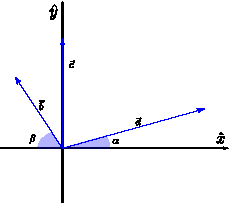
\includegraphics[scale=2.0]{vec_sum.pdf}
 \caption{Rappresentazione dei 3 vettori nel piano}
 \label{fig:vec_sum}
\end{figure}

Poniamoci nella situazione riportata in Figura \ref{fig:vec_sum}, così facendo il vettore $\vec{c}$ ha solo componente verticale e i calcoli saranno agevolati, abbiamo assegnato $\alpha$ e $\beta$ come variabili angolari del problema.\\
Esprimiamo adesso il vettore somma sommando i tre vettori per componenti:
%
\begin{equation*}
\vec{a}+\vec{b}+\vec{c}=(a_x+b_x)\hat{x}+(a_y+b_y+c)\hat{y}
\end{equation*}
%
Ricordiamo che per ottenere le componenti di un vettore rispetto ad uno degli assi di riferimento è sufficiente fare il prodotto scalare del vettore con il versore direttore dell'asse o equivalentemente ricorrere a relazioni trigonometriche (attenzione al verso della componente che, in questo ultimo caso, dovete stabilire voi). Avremo allora:
%
\begin{equation*}
\vec{a}+\vec{b}+\vec{c}=(a\cos\alpha-b\cos\beta)\hat{x}+(a\sin\alpha+b\sin\beta+c)\hat{y}
\end{equation*}
%
Calcoliamo adesso il modulo della risultante:
%
\begin{equation*}
\qty|\vec{a}+\vec{b}+\vec{c}|=\sqrt{(a\cos\alpha-b\cos\beta)^2+(a\sin\alpha+b\sin\beta+c)^2}
\end{equation*}
%
Ed infine il suo angolo rispetto all'asse $x$:
%
\begin{equation*}
\tan(\theta)= \frac{\qty(\vec{a}+\vec{b}+\vec{c})_y}{\qty(\vec{a}+\vec{b}+\vec{c})_x} =\frac{a\sin\alpha+b\sin\beta+c}{a\cos\alpha-b\cos\beta} \Rightarrow \theta= \arctan \qty( \frac{a\sin\alpha+b\sin\beta+c}{a\cos\alpha-b\cos\beta})
\end{equation*}
%
Con i valori dati nel testo si ha:
%
\begin{equation*}
\qty|\vec{a}+\vec{b}+\vec{c}|\approx 38.3\;\text{m} \qquad \qquad \theta \approx 75.1\degree
\end{equation*}
%

\subsection{Rotazione del sistema di riferimento \rstar\rstar}
Un punto P è descritto dalle coordinate $(p_x, p_y)$ rispetto al normale sistema di riferimento cartesiano $xOy$. Esprimete le coordinate di questo punto nel sistema di riferimento ruotato di un angolo $\theta$. In Figura \ref{fig:rotation} la situazione del problema. \\
\textit{Suggerimento}: dovrete ottenere delle espressioni in cui $p_{x'}$ dipende contemporaneamente da $p_x$ e $\theta$

\begin{figure}[h]
 \centering
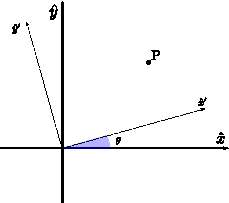
\includegraphics[scale=1.8]{rotation.pdf}
 \caption{Punto P e i due sistemi di riferimento, normale e ruotato}
 \label{fig:rotation}
\end{figure}


\subsubsection*{Soluzione}
Iniziamo col notare che una rotazione mantiene invariate le distanze fra punti, quindi il modulo del vettore $\qty|\vec{p}|=p$ rimarrà lo stesso sia nel sistema di riferimento normale sia in quello ruotato, riferiamoci a Figura \ref{fig:rotation_sol}

\begin{figure}[h]
 \centering
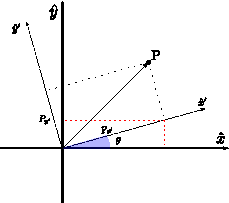
\includegraphics[scale=1.8]{rotation_sol.pdf}
 \caption{Scomposizioni di $\vec{p}$ in componenti ed ulteriore scomposizione di esse rispetto al sistema di riferimento normale}
 \label{fig:rotation_sol}
\end{figure}

Proiettiamo adesso le componenti di $\vec{p}$ del riferimento ruotato $(p_{x'},p_{y'})$ sul riferimento normale usando il comune procedimento, questo è quanto richiede l'esercizio:
%
\begin{gather*}
\vec{p}\cdot \hat{x}=p_{x}=p_{x'}\hat{x}'\cdot\hat{x}+p_{y'}\hat{y}'\cdot\hat{x}=p_{x'}\cos\theta+p_{y'}\cos(90\degree+\theta)=p_{x'}\cos\theta-p_{y'}\sin\theta\\
\vec{p}\cdot \hat{y}=p_{y}=p_{x'}\hat{x}'\cdot\hat{y}+p_{y'}\hat{y}'\cdot\hat{y}=p_{x'}\cos(90\degree-\theta)+p_{y'}\cos(\theta)=p_{x'}\sin\theta+p_{y'}\cos\theta\\
\end{gather*} 
%
A questo punto basterà risolvere il sistema di equazioni per le incognite $p_{x'},p_{y'}$, ottenendo:
%
\begin{gather*}
p_{x'}=p_{x}\cos\theta+p_{y}\sin\theta\\
p_{y'}=-p_{x}\sin\theta+p_{y}\cos\theta\\
\end{gather*} 
%
\textit{Un passo in più...}: Ricordando che  $\qty|\vec{p}|=\qty|\vec{p}'|$, le relazioni prima individuate possono essere riscritte per i versori direttori (che ricordiamo essere vettori dal modulo unitario), dividendo proprio per $\qty|\vec{p}|$:
%
\begin{gather*}
\frac{p_{x'}}{\qty|\vec{p}'|} =\frac{p_{x}}{\qty|\vec{p}|}\cos\theta+\frac{p_{y}}{\qty|\vec{p}|}\sin\theta\\
\frac{p_{y'}}{\qty|\vec{p}'|}=-\frac{p_{x}}{\qty|\vec{p}|}\sin\theta+\frac{p_{y}}{\qty|\vec{p}|}\cos\theta\\
\end{gather*} 
%
Ovvero, dalla definizione di versore $\hat{v}=\vec{v}/\qty|\vec{v}|$:
%
\begin{gather*}
\hat{x}'=\cos\theta\hat{x}+\sin\theta\hat{y}\\
\hat{y}'=-\sin\theta\hat{x}+\cos\theta\hat{y}
\end{gather*} 
%
Questa trasformazione del tutto generale dei versori ci permette di ottenere rapidamente le coordinate di un punto (e quindi di un vettore) in un asse cartesiano ruotato di un generico angolo $\theta$.
\\

\textit{Più frequentemente si trova scritta sui manuali l'espressione per una rotazione del punto tenendo fisso il sistema di riferimento, questa differisce solo per il segno davanti ai seni. Per chi volesse approfondire: quella fatta in questo esercizio è chiamata Outer Transformation, quella in cui viene ruotato il vettore invece è una Inner Transformation.}


\subsection{Somma, differenza e intensità relative \rstar\rstar\rstar}
Due vettori $\vec{a}$ e $\vec{b}$ hanno intensità uguali. Determinare l'angolo fra loro affinché l'intensità della somma $\vec{a} + \vec{b}$ sia più grande di un fattore $n$ rispetto alla differenza $\vec{a}-\vec{b}$. Risolvere per $n=10$\\
\textit{Suggerimento}: scegliere il sistema di riferimento in modo da ridurre al minimo il numero di componenti in gioco. \\
\textit{Avvertimento}: L'esercizio può creare qualche difficoltà algebrica, ma se tenete duro ad un certo punto ci saranno delle semplificazioni che renderanno tutto più agevole.

\subsubsection*{Soluzione}

\begin{figure}[h]
 \centering
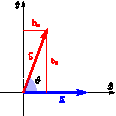
\includegraphics[scale=3.3]{sum_diff.pdf}
 \caption{Schema del problema, il vettore $\vec{a}$ è parallelo a un asse.}
 \label{fig:sum_diff}
\end{figure}

Scegliamo il riferimento come in Figura \ref{fig:sum_diff}, così da non avere componente verticale per il vettore $\vec{a}$. Calcoliamo le componenti della somma e della differenza dei vettori, ricordando che $\qty|\vec{a}|=\qty|\vec{b}|=a$:
%
\begin{gather*}
\vec{a} + \vec{b} = (a_x + b_x)\hat{x} + b_y\hat{y} = (a+a\cos\vartheta)\hat{x}+a\sin\vartheta\hat{y}  \\
\vec{a} - \vec{b} = (a_x - b_x)\hat{x} - b_y\hat{y} = (a-a\cos\vartheta)\hat{x}-a\sin\vartheta\hat{y} \\
\end{gather*} 
%
Adesso possiamo calcolare i moduli della somma e differenza: 
%
\begin{gather*}
\qty|\vec{a} + \vec{b}| = \sqrt{(a+a\cos\vartheta)^2 + a^2\sin^2\vartheta} = \sqrt{a^2+a^2(\cos^2\vartheta+\sin^2\vartheta)+2a^2\cos\vartheta}  \\
\qty|\vec{a} - \vec{b}| = \sqrt{(a-a\cos\vartheta)^2 + a^2\sin^2\vartheta} = \sqrt{a^2+a^2(\cos^2\vartheta+\sin^2\vartheta)-2a^2\cos\vartheta} \\
\end{gather*} 
%
Imponiamo infine la condizione data dall'esercizio
%
\begin{gather*}
\qty|\vec{a} + \vec{b}|/\qty|\vec{a} - \vec{b}|=n \\
\frac{2a^2+2a^2\cos\vartheta}{2a^2-2a^2\cos\vartheta} = n^2\\
\frac{1+\cos\vartheta}{1-\cos\vartheta}=n^2
\end{gather*} 
%
Risolvendo per $\cos\vartheta$ si ottiene:
%
\begin{equation*}
\cos\vartheta=\frac{n^2-1}{n^2+1}
\end{equation*}
%
Notiamo, come verifica del nostro buon procedere, che il valore letterale cui è uguagliato il coseno è sempre minore di 1.
Ricaviamo quindi $\vartheta$ e risolvere per il valore numerico fornito: 
%
\begin{equation*}
\vartheta=\arccos\qty(\frac{n^2-1}{n^2+1})\rightarrow \vartheta \approx 11\degree
\end{equation*}


\subsection{Pallina lanciata da una mongolfiera \rstar}
Da una mongolfiera una persona lancia orizzontalmente una pallina con velocità pari a $10.0\;\text{m/s}$, quale velocità iniziale (angolo e modulo) ha la palla rispetto a una persona ferma al suolo se la mongolfiera sta salendo con una velocità di $2\;\text{m/s}$? La situazione è riportata in Figura \ref{fig:mongolfiera}.

\begin{figure}[!ht]
\centering
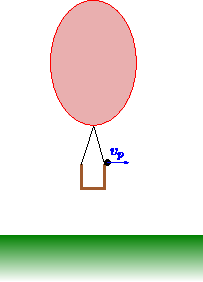
\includegraphics[scale=1.5]{mongolfiera.pdf}
\caption{Salita della mongolfiera con lancio orizzontale di una pallina. \label{fig:mongolfiera} }
\end{figure}

\subsubsection*{Soluzione}
Questo problema riguarda le velocità relative, scriviamo la nota relazione fra i sistemi di riferimenti fermo O e quello solidale con la mongolfiera O':
%
\begin{gather*}
\vec{v}=\vec{v}_{O'}+\vec{v}'
\end{gather*}
%
Con $\vec{v}$ velocità misurata rispetto al sistema fisso O, $\vec{v}_{O'}$ è la velocità del sistema mobile e $\vec{v}'$ è la velocità dell'oggetto misurata nel sistema di riferimento mobile O'. Quindi avremo $\vec{v}_{O'}=\vec{v}_{m}$ e $\vec{v}'=\vec{v}_{p}$. Dunque la velocità della pallina da terra sarà:

%
\begin{gather*}
\vec{v}=\vec{v}_{m}+\vec{v}_{p}=v_p\hat{x}+v_m\hat{y}
\end{gather*}
%
Si può allora calcolare facilmente calcolare modulo e angolo della velocità della pallina vista da terra:
%
\begin{gather*}
\qty|\vec{v}|=\sqrt{v_p^2+v_m^2}\approx 10.20 \frac{\text{m}}{\text{s}}\\
\tan\theta=\frac{v_m}{v_p} \Rightarrow \theta=\arctan\qty(\frac{v_m}{v_p})\approx 11.31 \degree
\end{gather*}
%

\subsection{Passeggero su battello \rstar}
Un passeggero di un battello che ha una velocità di $2.70\;\text{m/s}$ sale una rampa di scale per raggiungere il ponte principale con una velocità di $0.75\;\text{m/s}$. Le scale formano un angolo di 45° rispetto alla direzione del moto, la situazione è schematizzata in Figura \ref{fig:boat}. Qual è la velocità del passeggero rispetto all'acqua (rispondere in modulo e angolo)?

\begin{figure}[!ht]
\centering
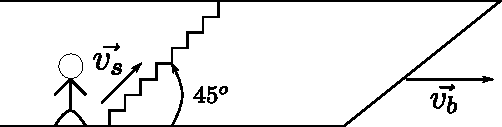
\includegraphics[scale=1]{boat.pdf}
\caption{Velocità del battello $\vec{v_b}$ e del passeggero sulla scala $\vec{v_s}$ \label{fig:boat} }
\end{figure}

\subsubsection*{Soluzione}
Siamo di fronte ad un classico problema di velocità relative. La relazione che ci permette di esprimere la velocità di un oggetto rispetto ad un sistema di riferimento O fisso è la seguente:
%
\begin{gather*}
\vec{v}=\vec{v}_{O'}+\vec{v}'
\end{gather*}
%
Dove $\vec{v}$ è la velocità misurata rispetto al sistema di riferimento fisso O, $\vec{v}_{O'}$ è la velocità del sistema di rifermento mobile e $\vec{v}'$ è la velocità dell'oggetto misurata nel sistema di riferimento mobile O'. Nel nostro caso avremo quindi:
%
\begin{gather*}
\vec{v}_{s,O}=\vec{v_b}+\vec{v_s}=(v_s\cos45\degree+v_b)\hat{x}+(v_s\sin45\degree)\hat{y}=(v_s\frac{\sqrt{2}}{2}+v_b)\hat{x}+(v_s\frac{\sqrt{2}}{2})\hat{y}
\end{gather*}
%
Si può calcolare facilmente il modulo:
%
\begin{gather*}
\qty|\vec{v}_{s,O}|=\sqrt{(v_s\frac{\sqrt{2}}{2}+v_b)^2+\frac{1}{2}v_s^2}=\sqrt{v_s^2+v_b^2+\sqrt{2}v_s v_b} \approx 3.27\;\frac{\text{m}}{\text{s}}
\end{gather*}
%
E l'angolo con l'asse $x$:
%
\begin{gather*}
\sin\theta=\frac{v_s\frac{\sqrt{2}}{2}}{\qty|\vec{v}_{s,O}|} \Rightarrow \theta\approx 9.33\degree
\end{gather*}
%


\chapter{Cinematica}
\section{Esercizi}

\subsection*{Esercizio 1}
Un segmento rettilineo delimitato da due punti $A$ e $B$ è lungo $\Delta x=230$ km. Un punto materiale  si muove di moto rettilineo uniforme da $A$ verso $B$.  Qual è la sua \textit{velocità scalare media} $\bar{v}$  se percorre il tratto in un tempo $\Delta t =3.25$ h? Esprimere il risultato in km/h e in m/s.
 
\subsubsection*{Soluzione}
Poniamo $\Delta x = 230$ km e $\Delta t = 3.25$ h. Allora, dalla definizione di velocità media ricaviamo subito:
\begin{equation*}
\bar{v}= \frac{\Delta x}{\Delta t}=\frac{230 \;\text{ km}}{3.25 \; \text{h}}\simeq 70.77\;  \frac{\text{ km}}{\text{h}}
\end{equation*}\\
Per convertire da km/h a m/s ricordiamo che $1$h=$3600$s e quindi:
\begin{equation*}
\frac{\text{ km}}{\text{h}}=\frac{1000 \text{ m}}{3600\text{s}}=\frac{1}{3.6}\;\frac{\text{m}}{\text{s}}
\end{equation*}\\
La conversione delle velocità da km/h a m/s comporta dunque una divisione per un fattore 3.6. Il risultato richiesto è dunque:\\
\begin{equation*}
\bar{v}\simeq \frac{70.77}{3.6} \frac{\text{m}}{\text{s}} \simeq \;   19.66 \frac{\text{m}}{\text{s}}
\end{equation*}\\

\subsection*{Esercizio 2}
Un cavallo si allontana dal suo addestratore percorrendo in linea retta $130$ m in $14$ s. Subito dopo si gira improvvisamente e torna al galoppo verso l'addestratore, percorrendo metà della distanza in $4.8$ s. Considerando come positivo il verso della velocità del cavallo quando questi si allontana dall'addestratore
e supponendo che la velocità del cavallo sia costante in ogni tratto, determinare:
\begin{enumerate}
\item[a.]{il modulo della velocità del cavallo quando si allontana ($v_1$);}
\item[b.]{il modulo della velocità del cavallo quando torna indietro ($v_2$);}
\item[c.]{la \textit{velocità scalare media} $\bar{v}_{\text{scalare}}$ nell'intero percorso;}
\item[d.]{la \textit{velocità vettoriale media} $\bar{v}_{\text{vettoriale}}$ nell’intero percorso.}
\end{enumerate}

\subsubsection*{Soluzione}
Poniamo: $\Delta x_1 = 130 \;$ m, $t_1 = 14 \;$ s, $\Delta x_2 = \frac{\Delta x_1}{2}= 65 \;$ m e $t_2 = 4.8 \;$ s. \\
\emph{a)} La velocità del cavallo nel primo tratto è data da:
\begin{equation*}
v_1=\frac{\Delta x_1}{t_1}= \frac{130 \; \text{m}}{14 \; \text{s}} \simeq 9.28 \frac{\text{m}}{\text{s}} 
\end{equation*}
\emph{b)} La velocità media del cavallo nel secondo tratto è data da:
\begin{equation*}
v_2=\frac{\Delta x_2}{t_2}= \frac{65 \; \text{m}}{4.8 \; \text{s}} \simeq 13.54 \frac{\text{m}}{\text{s}} 
\end{equation*}
\emph{c)} Per calcolare la velocità scalare media utilizziamo la definizione:
\begin{equation*}
\bar{v}_{\text{scalare}}=\frac{\text{spazio  totale percorso}}{\text{tempo totale trascorso}}=\frac{\Delta x_1 + \Delta x_2}{t_1 + t_2}= \frac{130 + 65}{14 + 4.8} \: \frac{\text{m}}{\text{s}}\simeq 10.37 \; \frac{\text{m}}{\text{s}}
\end{equation*}
\emph{d)} Per calcolare la velocità vettoriale media utilizziamo la sua definizione:
\begin{equation*}
\bar{v}_{\text{vettoriale}}=\frac{\text{spostamento totale}}{\text{tempo  totale  trascorso}}= \frac{\text{posizione  finale - posizione iniziale}}{\text{tempo  totale  trascorso}}	
\end{equation*}
e quindi:
\begin{equation*}
\bar{v}_{\text{vettoriale}}=\frac{\Delta x_1 - \Delta x_2}{t_1 + t_2}= \frac{130 - 65}{14 + 4.8}\frac{m}{s}\simeq 3.46 \; \frac{\text{m}}{\text{s}} 
\end{equation*}
Il segno $-$ è dovuto al fatto che il cavallo percorre il tratto iniziale
con velocità positiva, mentre percorre il secondo tratto con verso opposto.\\


\subsection*{Esercizio 3}
Due locomotive si muovono su due binari rettilinei fra loro paralleli. Entrambe partono al tempo $t=0$, una dalla posizione $x=0$ e l’altra dalla posizione $x_0=8.5$ km. La prima procede ad una velocità costante di $+20$ km/h, l’altra a una velocità costante di $-30$ km/h. Dopo quanto tempo si incontreranno? In che punto si incontreranno? Esprimere i risultati rispettivamente in secondi e in km.

\subsubsection*{Soluzione}
Dalla teoria del moto rettilineo uniforme, sappiamo che la legge oraria di un corpo che parte da un punto $x_0$ con velocità costante $v$ è data da:\\
\begin{equation*}
x(t)=x_0+vt
\end{equation*}
Le leggi orarie delle locomotive sono quindi rispettivamente:
\begin{gather*}
x_1(t)=v_1 t \\
x_2(t)=x_0 - v_2 t
\end{gather*}
dove $v_1=+20$ km/h e $v_2=+30$ km/h. Affinché le locomotive si incontrino deve esistere un tempo $t^*$ in cui le coordinate $x$ delle due locomotive sono uguali, ovvero:\\
\begin{equation*}
x_1 (t^*) = x_2(t^*) \quad \Rightarrow \quad v_1  t^* = x_0 - v_2  t^* 
\end{equation*}
da cui, ricavando $t^*$:\\
\begin{equation*}
t^* = \frac{x_0}{v_1 + v_2} = \frac{8.5}{20 +30} \; \text{h} \simeq 0.17 \; \text{h} = 0.17 \cdot 3600 \; \text{s} \simeq 612 \; \text{s}
\end{equation*}
Il punto $x^*$ di incontro di trova inserendo $t^*$ in una delle due leggi orarie, per esempio nella prima: 
\begin{gather*}
x_1(t^*)=v_1 t^*= \frac{v_1}{v_1 + v_2} x_0= \frac{2}{5}x_0=3.4 \; \text{ km}
\end{gather*}

\subsection*{Esercizio 4}
Alcuni amici partono per un viaggio con due macchine. La prima parte al tempo $t=0$ e procede a una velocità costante di $24$ m/s; la seconda parte $100\;\text{s}$ dopo la prima. A $12$ km dal punto di partenza c’è un bivio. Quale deve essere la velocità $v_1$ della seconda macchina affinché questa raggiunga la prima macchina al bivio? Al bivio si accorgono di non aver portato la cartina e decidono di tornare insieme al punto di partenza. Percorsi 8 km in 300 s, ritrovano la cartina e si fermano. Calcolare la velocità scalare media $\bar{v}$ e la velocità vettoriale media $v_m$ di entrambe le macchine.

\subsubsection*{Soluzione}
\emph{a)} Calcoliamo innanzitutto quanto tempo impiega la prima macchina ad arrivare al bivio. Il tempo $t_0$ impiegato a percorrere la distanza $\Delta x_1 = 12 \; \text{km} = 1.2 \cdot 10^4 \; \text{m}$ che la separa dal bivio, procedendo alla velocità costante $v_0 = 24 \;$ m/s sarà uguale a:\\
\begin{equation*}
t_0 = \frac{\Delta x}{v_0}= \frac{1.2 \cdot 10^4}{24} \; \text{s} = 500 \; \text{s}
\end{equation*}\\
La seconda macchina parte con $\Delta t = 100 \; s$ di ritardo rispetto alla prima. Affinché le due macchine arrivino assieme, la seconda macchina dovrà perciò percorrere i $12$ km dal punto di partenza al bivio in $t_1=t_0-\Delta t = 400 \; s$. Imponendo questa condizione, ricaviamo la velocità media $v_1$ della seconda macchina:\\
\begin{equation*}
v_1= \frac{\Delta x_1}{t_1}=\frac{\Delta x_1}{t_0 - \Delta t}= \frac{1.2 \cdot 10^4}{400}\frac{\text{m}}{\text{s}} = 30 \; \frac{\text{m}}{\text{s}}
\end{equation*}\\
\emph{b)} Le due macchine percorrono $\Delta x_2=8 \;$ km$ = 8\cdot 10^3 \;$ m in $t_2=300 \;$ s, quindi la loro velocità media $v_2$ equivale a:\\
\begin{equation*}
v_2=\frac{\Delta x_2}{t_2}=\frac{8\cdot 10^3}{300} \: \frac{\text{m}}{\text{s}}=26.7 \: \frac{\text{m}}{\text{s}}
\end{equation*}\\
Possiamo allora calcolare le velocità richieste:
\begin{itemize}
\item{la velocità scalare media della prima macchina vale:\\
\begin{equation*}
\bar{v}_1 = \frac{\Delta x_1 + \Delta x_2}{t_0 + t_2}= \frac{1.2\cdot 10^4 + 8\cdot 10^3}{500 + 300} \: \frac{\text{m}}{\text{s}}= 25.00 \: \frac{\text{m}}{\text{s}}
\end{equation*}}
\item{la velocità scalare media della seconda macchina vale:\\
\begin{equation*}
\bar{v}_2 = \frac{\Delta x_1 + \Delta x_2}{t_1 + t_2}= \frac{1.2\cdot 10^4 + 8\cdot 10^3}{400 + 300} \: \frac{\text{m}}{\text{s}}\simeq 28.57 \: \frac{\text{m}}{\text{s}}
\end{equation*}}
\item{la velocità vettoriale media della prima macchina vale:\\
\begin{equation*}
v_{m1} = \frac{\Delta x_1 - \Delta x_2}{t_0 + t_2}= \frac{1.2\cdot 10^4 - 8\cdot 10^3}{500 + 300} \: \frac{\text{m}}{\text{s}}= 5.00 \: \frac{\text{m}}{\text{s}}
\end{equation*}}
\item{la velocità vettoriale media della prima macchina vale:\\
\begin{equation*}
v_{m2} = \frac{\Delta x_1 - \Delta x_2}{t_1 + t_2}= \frac{1.2\cdot 10^4 - 8\cdot 10^3}{400 + 300} \: \frac{\text{m}}{\text{s}}\simeq 5.71 \: \frac{\text{m}}{\text{s}}
\end{equation*}}
\end{itemize}


\subsection*{Esercizio 5}
Un aeroplano percorre $3100$ km a una velocità costante di $790$ km/h; poi incontra un vento di coda che fa aumenteare la sua velocità di $990$ km/h per i successivi $2800$ km. Qual è la durata complessiva del viaggio? Qual è la velocità scalare media dell'aeroplano in questo viaggio?

\subsubsection*{Soluzione}
Il tempo $\Delta t$ necessario a coprire una distanza $\Delta x$ con una velocità $v$ è ovviamente:
\begin{equation*}
\Delta t= \frac{\Delta x}{v}
\end{equation*}
quindi il nostro aereo percorrerà la prima tratta in un tempo:
\begin{equation*}
t_{1}=\frac{3100 \text{km}}{790 \text{km/h}}\simeq3.92\;\text{h}
\end{equation*}
e la seconda tratta in un tempo:
\begin{equation*}
t_{2}=\frac{2800 \text{km}}{(790+990) \text{km/h}}\simeq1.57 \;\text{h}
\end{equation*} 
La durata complessiva del viaggio è dunque $t_{tot}= t_{1}+t_{2}= 5.49 h$. Usando la definizione di velocità scalare media, troviamo:
\begin{equation*}
\bar{v}=\frac{\text{spazio  totale percorso}}{\text{tempo totale trascorso}}= \frac{(3100+2800) \text{km} }{5.49 \text{h}}=1075\; \frac{\text{km}}{\text{h}}
\end{equation*}


\subsection*{Esercizio 6} 
Una palla da bowling che viaggia con velocità costante $v$ coplisce i birilli posti in fondo ad una pista da bowling lunga $16.5$ m. Il giocatore sente il rumore della palla che colpisce i birilli $2.50$ s dopo che la palla ha lasciato la sua mano. Quanto valeva $v$? Si assuma un valore della velocità del suono pari a $v_s\simeq340$ m/s.

\subsubsection*{Soluzione}
Possiamo pensare al suono come ad un'onda d'urto che si genera nell'istante in cui avviene lo scontro fra la palla e i birilli e che si propaga nell'aria con velocità $v_{s}\simeq340$ m/s. Il giocatore $sente$ il suono dei birilli che cadono nel momento in cui l'onda raggiunge il suo orecchio.\\
Il tempo che trascorre tra il lancio della palla e il momento in cui il giocatore sente il botto dei birilli è dunque:
\begin{equation}
t_{0}=t_{palla}+t_{suono}=2.50 \; \text{s}
\label{eq:6.1}
\end{equation}
dove $t_{palla}$ è il tempo necessario alla palla per percorrere tutta la pista ($\Delta x=16.5$ m) e $t_{suono}$ è il tempo necessario all'onda sonora (generata dallo scontro fra palla e birilli) per arrivare all'orecchio del giocatore (e quindi a ripercorrere nuovamente tutta la lunghezza della pista $\Delta x$). Applicando le leggi orarie possiamo scrivere:
\begin{equation}
t_{suono}=\frac{\Delta x}{v_s}=\frac{16.5 \text{m}}{340 \frac{\text{m}}{\text{s}}}\simeq 0.05 \; \text{s}
\label{eq:6.2}
\end{equation}
e:
\begin{equation}
t_{palla}=\frac{\Delta x}{v_{palla}}=\frac{16.5 \text{m}}{v_{palla}}.
\label{eq:6.3}
\end{equation}
Sostituendo la \ref{eq:6.2} e la \ref{eq:6.3} nella \ref{eq:6.1} otteniamo un'equazione che ha come incognita $v_{palla}$:
\begin{equation*}
\frac{16.5 \text{m}}{v_{palla}}+0.05 \text{s}=2.50 \; \text{s};
\end{equation*}
dunque:
\begin{equation*}
v_{palla}=\frac{16.5 \text{m}}{(2.50-0.05) \text{s}}=6.7 \; \frac{\text{m}}{\text{s}}
\end{equation*}

\subsection*{Esercizio 7} 
Un'automobile che viaggia su un rettilineo alla velocità costante di $95\;\text{km/h}$ sorpassa una treno lungo $1.1\;\text{km}$ che va nella stessa direzione su un binario parallelo alla strada. Se la velocità del treno è costante e pari a $75\;\text{km/h}$, quanto tempo impiegherà l'auto a superarlo e quale distanza avrà percorso in questo intervallo di tempo? Come cambiano i risultati se il treno viaggia con la velocità in modulo uguale a prima ma con verso opposto rispetto a quella dell'auto?

\subsubsection*{Soluzione}
Scriviamo le leggi orarie per l'automobile $x_{\text{auto}}(t)$ e per il treno $x_{\text{treno}}(t)$. Facciamo attenzione a definire le posizioni iniziali: possiamo stabilire che a $t=0$ $x_{\text{auto}}=0$ e $x_{\text{treno}}=1100\;\text{m}$. Ricaviamo quindi:
\begin{eqnarray*}
      x_{\text{auto}}(t)=v_{\text{auto}}t\\ 
   x_{\text{treno}}(t)= x_{\text{treno}}(0)+v_{\text{treno}}t
  \end{eqnarray*}
Imponendo: $x_{\text{auto}}(t_{\text{sorpasso}})=x_{\text{treno}}(t_{\text{sorpasso}})$ troviamo $t_{sorpasso}$, ovvero il tempo necessario all'auto per superare il treno:
\begin{equation*}
t_{\text{sorpasso}}=\frac{x_{\text{treno}}(0)}{v_{\text{auto}}-v_{\text{treno}}}=\frac{1100 \;\text{m}}{5.5\;\text{m/s}}=200\;\text{s}
\end{equation*}
In questo tempo l'auto avrà percorso uno spazio pari a:
\begin{equation*}
x_{\text{auto}}(t_{\text{sorpasso}})=v_{\text{auto}}t_{\text{sorpasso}}=5.3 \; \text{km}
\end{equation*}
Se il treno avesse avuto la stessa velocità di prima ma direzione opposta al moto della macchina, ovviamente sia $t_{sorpasso}$ che $x_{\text{auto}}(t_{\text{sorpasso}})$ sarebbero stati più piccoli:
\begin{equation*}
t_{\text{sorpasso}}=\frac{x_{\text{treno}}(0)}{v_{\text{auto}}+v_{\text{treno}}}=\frac{1100 \text{m}}{47.22 \text{m/s}}=23.3 \;\text{s}
\end{equation*}
e:
\begin{equation*}
 x_{\text{auto}}(t_{\text{sorpasso}})=v_{\text{auto}}t_{\text{sorpasso}}=615\; \text{m}
\end{equation*}

\subsection*{Esercizio 8}
Un treno parte da una stazione da fermo e percorre, con accelerazione $a$ costante, 1.5 km in 90 s lungo un rettilineo. Quanto vale $a$? A 90 s dalla partenza, qual è la sua velocità $v$? E la velocità media $\bar{v}$ fino a quel momento?

\subsubsection*{Soluzione}
\emph{a)} Volendo esprimere il risultato nelle unità fondamentali poniamo $d=1.5 \; \text{km} = 1.5 \cdot 10^3 \; \text{m}$ la distanza percorsa dal treno in $t^*=90 \; \text{s}$ e calcoliamo quale deve essere la sua accelerazione affinché ciò avvenga. Partendo dalla legge oraria per il moto uniformemente accelerato, imponiamo:\\
\begin{equation*}
d=x_0+v_0 t^* + \frac{1}{2}a (t^*)^2 = \frac{1}{2} a (t^*)^2
\end{equation*}
Nel nostro caso, infatti, $x_0 =0$ e $v_0 = 0$, perché il treno parte da fermo e poniamo l'origine dell'asse $x$ coincidente col punto di partenza del treno. Ricaviamo $a$ dalla precedente equazione:\\
\begin{equation*}
a= \frac{2d}{(t^*)^2}= \frac{3 \cdot 10^3}{(90)^2} \frac{\text{m}}{\text{s}^2}\simeq 0.37 \; \frac{\text{m}}{\text{s}^2}
\end{equation*}
\emph{b)} Una volta nota l'accelerazione del treno, possiamo calcolare quale sia la sua velocità dopo un tempo $t^*$ dalla partenza:\\
\begin{equation*}
v(t^*) = v_0 + a t^* = a t^* \simeq 0.37\cdot 90 \frac{\text{m}}{\text{s}} \simeq 33.3 \; \frac{\text{m}}{\text{s}}
\end{equation*}
\emph{c)} Dalla definizione di velocità media, sappiamo che:\\
\begin{equation*}
\bar{v}= \frac{\text{spazio  percorso}}{\text{tempo  trascorso}}=\frac{d}{t^*}=\frac{1.5 \cdot 10^3}{90}\frac{\text{m}}{\text{s}}\simeq16.6\; \frac{\text{m}}{\text{s}}
\end{equation*}

\subsection*{Esercizio 9}
Un aeroplano leggero deve raggiungere una velocità di 30 m/s per poter decollare. Se la sua accelerazione è di $3 $ m/s$^2$ costante, quanto deve essere la lunghezza minima della pista per permettere il decollo?

\subsubsection*{Soluzione}
Cominciamo a calcolare dopo quanto tempo l'aeroplano, partendo da fermo ($v_0=0$) con accelerazione $a=3 \; \text{m/s}^2$ costante, raggiunge la velocità richiesta $V = 30 \;\text{m/s}$:
\begin{equation*}
V=at \Longrightarrow t=\frac{V}{a}=\frac{30}{3}\; \text{s} = 10 \; \text{s}
\end{equation*}\\
Quanto spazio ha percorso l'aeroplano in questo tempo? Poniamo il punto di partenza a $x_0 = 0$. Allora:\\
\begin{equation*}
x(t)= x_0 + v_0  t + \frac{1}{2}a t^2 = \frac{1}{2}a  t^2 = \frac{1}{2}\cdot 3 \cdot 10^2 \; \text{m} = 150 \; \text{m}
\end{equation*}\\
quindi la pista deve essere lunga almeno 150 m per permettere all'aeroplano di decollare.\\


\subsection*{Esercizio 10}
Una macchina viaggia di moto rettilineo uniforme alla velocità di 100 km/h lungo un rettilineo. All'istante $t=0$ inizia a frenare con un'accelerazione costante di $-20\;\text{m/s}^2$  fino a fermarsi completamente. A che istante di tempo si ferma? E quanto spazio ha percorso? Ripetere i calcoli nel caso in cui la macchina abbia velocità iniziale di 200 km/h.

\subsubsection*{Soluzione}
Come prima cosa, conviene convertire la velocità della macchina in $m/s$:\\
\begin{equation*}
v_0=100 \: \frac{\text{km}}{\text{h}}= \frac{100}{3.6}\:\frac{\text{m}}{\text{s}}\simeq 27.8 \; \frac{\text{m}}{\text{s}}
\end{equation*}\\
A questo punto possiamo calcolare il tempo richiesto, che equivale al tempo $t$ impiegato per portare la velocità $v(t)$ da $v_0$ a $0$:\\
\begin{equation*}
v(t)=v_0+at=0 \Longrightarrow t= - \frac{v_0}{a}= -\frac{27.8}{-20} \: \text{s} = 1.4 \; \text{s}
\end{equation*}\\
In tale tempo, ponendo $x_0=0$ la posizione nel momento in cui il guidatore inizia a frenare, lo spazio percorso dalla macchina sarà:\\
\begin{equation*}
x(t)=x_0 + v_0 t + \frac{1}{2} a t^2 = \big(0 + 27.8 \cdot 1.4 + \frac{1}{2} \cdot (-20) \cdot (1.4)^2 \big) \: m \simeq 19.3 \; \text{m}
\end{equation*}\\
 
Nel caso in cui la velocità iniziale fosse stata 200 km/h:
\begin{equation*}
t_{\text{frenata}}\simeq -\frac{55.5}{-20}\text{s}\simeq 2.8 \; \text{s}
\end{equation*}
mentre
\begin{equation*}
x_{\text{frenata}}=(55.5\cdot 2.8-\frac{1}{2} 20\cdot (2.8)^2)\text{m}\simeq 77 \; \text{m}
\end{equation*}
Notiamo che raddoppiando la velocità iniziale il tempo di frenata è raddoppiato a sua volta, ma lo spazio di frenata è $quadruplicato$!

\subsection*{Esercizio 11}
Un proiettile viene sparato verticalmente \textit{verso l'alto} con velocità iniziale pari a 392 m/s. Calcolare l'altezza massima raggiunta e il tempo impiegato (accelerazione di gravità $g = 9.8 \; m/s^2$).

\subsubsection*{Soluzione}
Una volta sparato a velocità iniziale $v_0 = 392 \:$ m/s, il proiettile segue le leggi del moto uniformemente accelerato con accelerazione costante $g=-9.8 \:$ m/s$^2$ (il segno meno è dovuto al fatto che l'accelerazione è diretta in verso opposto alla velocità iniziale del  proiettile). Nel salire, il proiettile rallenterà sempre più fino a fermarsi, per poi cominciare a discendere. Il punto di massima altezza sarà allora quello in cui la velocità del proiettile è nulla. Calcoliamo dopo quanto tempo il proiettile si arresta:\\
\begin{equation*}
v(t)= v_0 + g t =0 \Longrightarrow t= -\frac{v_0}{g}= -\frac{392}{- 9.8} \: \text{s} \simeq 40 \;  \text{s}
\end{equation*}\\
Qual è l'altezza massima raggiunta? Possiamo ricavarla utilizzando l'equazione del moto per il proiettile, ponendo $h_0 = 0$ il punto da cui viene sparato il proiettile, e calcolando quanto valga lo spazio $h(t)$ percorso nel tempo $t$ che abbiamo appena calcolato:\\
\begin{equation*}
h(t) = v_0 t + \frac{1}{2}g t^2 = \left( 392 \cdot 40 - \frac{1}{2} \cdot 9.8 \cdot (40)^2 \right) \: \text{m} = 7840 \; \text{m} 
\end{equation*}

\subsection*{Esercizio 12}
Una macchina da corsa parte da ferma, accelera per 5 secondi con un'accelerazione di 8 m/s$^2$, mantiene la velocità raggiunta per altri 5 secondi e poi frena con un'accelerazione pari a $-10 \; \text{m/s}^2$ fino a fermarsi. Quanto spazio ha percorso in tutto?

\subsubsection*{Soluzione}
Lo spostamento totale sarà somma di tre termini:
\begin{itemize}
\item{Il primo, percorso ad accelerazione costante $a_1 = 8 \; \text{m/s}^2 $ e partendo da fermo, per $\Delta t_1 = 5\;$ s;}
\item{Il secondo, percorso a velocità costante $v_2$ (che dovremo calcolare), per $\Delta t_2 = 5\;$ s;}
\item{Il terzo, percorso con decelerazione costante $a_2 = -10 \;\text{m/s}^2$ che dura fino a fermarsi, quindi un tempo $\Delta t_3$ che dovremo calcolare.}
\end{itemize}
Calcoliamo il primo tratto:\\
\begin{equation*}
\Delta x_1 = \frac{1}{2} a_1 (\Delta t_1)^2 = \frac{1}{2}\cdot 8 \cdot (5)^2 \; \text{m} = 100 \; \text{m}
\end{equation*}\\
Per calcolare il secondo contributo, dobbiamo calcolare $v_2$. Dobbiamo allora capire che velocità ha raggiunto il veicolo dopo che è trascorso $\Delta t_1$. Calcoliamo:\\
\begin{equation*}
v_2 = a_1 \Delta t_1 = 8 \cdot 5 \; \frac{\text{m}}{\text{s}} = 40 \;\frac{\text{m}}{\text{s}}
\end{equation*}\\
A questo punto siamo pronti a calcolare il secondo tratto:\\
\begin{equation*}
\Delta x_2 = v_2 \Delta t_2 = 40 \cdot 5 \; \text{m} = 200 \; \text{m}
\end{equation*}\\

Per il terzo contributo, è invece necessario capire in quanto tempo il veicolo, avendo velocità iniziale $v_2$, si arresta sotto l'azione di una decelerazione costante $a_3$. Imponiamo allora che dopo un certo $\Delta t_3$ dall'inizio della frenata la velocità del veicolo sia nulla:\\
\begin{equation*}
v(\Delta t_3) = 0 = v_2 + a_3 \cdot \Delta t_3 \Longrightarrow \Delta t_3 = - \frac{v_2}{a_3}= -\frac{40}{- 10} \; s = 4 \; \text{s}
\end{equation*}\\
A questo punto possiamo calcolare il terzo tratto:\\
\begin{equation*}
\Delta x_3 = v_2 \cdot \Delta t_3 + \frac{1}{2} \cdot a_3 \cdot (\Delta t_3)^2 = \left( 40 \cdot 4 + \frac{1}{2} \cdot (-10) \cdot (4)^2 \right) \; \text{m} = 80 \;\text{m}
\end{equation*}\\

Infine, lo spostamento totale sarà:\\
\begin{equation*}
\Delta x_{tot} = \Delta x_1 + \Delta x_2 + \Delta x_3 = 380 \; \text{m}
\end{equation*}


\subsection*{Esercizio 13}  
Determinare la distanza di arresto per un'automobile con una velocità iniziale di $95$ km/h e un tempo di reazione umana di $1.0 s$: (a) per un'accelerazione $a=-4.0$ m/s$^{2}$; (b) per $a=-8.0$ m/s$^{2}$.

\subsubsection*{Soluzione}
La distanza di arresto è composta da due termini: $\Delta x_{tot}=\Delta x_{\text{reazione}}+\Delta x_{\text{frenata}}$. Il primo è dovuto alla distanza percorsa alla velocità costante di $95 km/h$ nel secondo di reazione del guidatore.
\begin{equation}
\Delta x_{\text{reazione}}=26.4 \; \frac{\text{m}}{\text{s}}\cdot 1.0 \;\text{s}=26.4 \;\text{m}.
\end{equation}
$\Delta x_{frenata}$ invece si ricava dalle equazioni del moto accelerato: dall'equazione
\begin{equation*}
v(t)=v(0)+a t,
\end{equation*}
imponendo $v(t_{\text{frenata}})=0$, trovo il tempo di frenata:
\begin{equation}
t_{\text{frenata}}=-\frac{v(0)}{a}.
\label{eq:13.1}
\end{equation}
D'altra parte, possiamo dire:
\begin{equation}
\Delta x_{\text{frenata}}= x(t_{\text{frenata}})-x_{0}= v t_{\text{frenata}}- \frac{1}{2}a t_{\text{frenata}}^2
\label{eq:13.2}
\end{equation}
e, sostituendo \ref{eq:13.1} in \ref{eq:13.2}, troviamo:
\begin{equation}
\Delta x_{\text{frenata}}=- v(0)\frac{v(0)}{a}+\frac{1}{2}a \left (\frac{v(0)}{a}\right )^2=-\frac{v(0)^2}{a}+\frac{1}{2}\frac{v(0)^{2}}{a}=-\frac{1}{2}\frac{v(0)^2}{a}.
\label{eq:13.3}
\end{equation}
Nel caso $a=-4.0$ m/s$^2$ la \ref{eq:13.3} ci dà il risultato:
\begin{equation*}
\Delta x_{tot}=\Delta x_{\text{reazione}}+\Delta x_{\text{frenata}}=(26.4+87.0) m=113.4 \;\text{m}
\end{equation*}
mentre nel caso $a=-8.0$ m/s$^2$:
\begin{equation*}
\Delta x_{tot}=\Delta x_{\text{reazione}}+\Delta x_{\text{frenata}}=(26.4+43.5) \text{m}=69.9 \; \text{m}
\end{equation*}

\subsection*{Esercizio 14}
Una lumaca si muove lungo una pista di sabbia rettilinea. La retta lungo la quale si sposta è indicata dal versore $\hat{x}$ di un sistema di riferimento cartesiano. All'istante iniziale $t_i=0$ s essa si trova nel punto $x_i=0$.  Subito dopo inizia a spostarsi e la sua velocità all'istante $t$ generico è: $\vec{v}(t)=v(t)\hat{x}$. Un naturalista si interessa del movimento della lumaca tra $t_i=0$ e $t_f=8.0\;\text{s}$ e traccia un grafico mettendo sulle ascisse il tempo $t$ (in $s$) e sulle ordinate la velocità $v(t)$ (in cm/s). Il risultato è riportato in Figura \ref{fig:lumaca}. Che tipo di moto caratterizza la lumaca nei tratti $a, b, c, d, e, f, g, h$? Qual è la massima velocità raggiunta dalla lumaca? Esprimerla in m/s e km/h. Qual è la massima accelerazione raggiunta dalla lumaca? Esprimerla in m/s$^2$ e km/h$^2$.  Sapete dire in quale punto $x_f$ si trova la lumaca a $t=t_f$? Qual è stata la sua \textit{velocità vettoriale media}? Quanta distanza ha coperto in totale?

 \begin{figure}[!ht]
 \centering
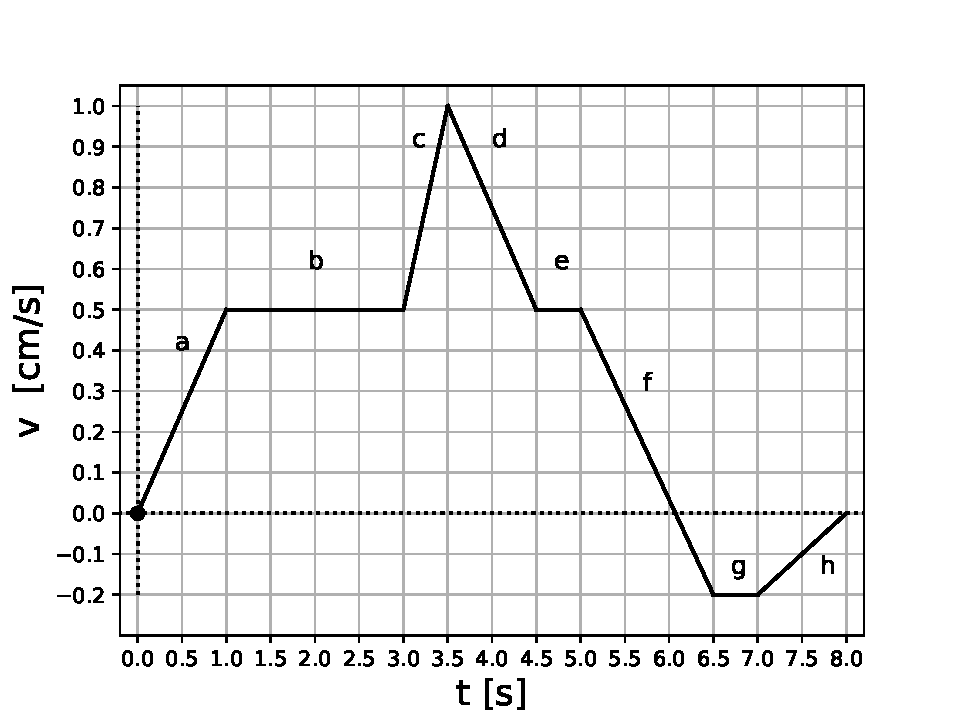
\includegraphics[scale=0.65]{lumaca.pdf}
\caption{Grafico $t$ (ascisse)/$v(t)$ (ordinate)  per il moto della lumaca oggetto dell'esercizio. \label{fig:lumaca} }
\end{figure}

\subsubsection*{Soluzione}
Nei tratti $b$, $e$, $g$ la velocità $v(t)$ è costante, quindi il moto è rettilineo uniforme. Nei tratti $a$, $c$, $d$, $f$, $h$ l'andamento di $v(t)$ è dato una retta, per cui $v(t)=at + \text{cost}.$ e il moto è uniformemente accelerato. (NB in effetti un moto rettilineo unifome è un moto uniformemente accelerato con $a=0$). Le accelerazioni nei tratti $a$, $c$, $d$, $f$, $h$ sono rispettivamente: 
\begin{gather*}
a_a=\frac{0.5 \; \text{cm/s}}{1 \; \text{s}}=0.5  \;\text{cm/s}^2 \qquad a_c=\frac{0.5 \; \text{cm/s}}{0.5 \;\; \text{s}}=1 \; \;\text{cm/s}^2 \qquad a_d=\frac{-0.5 \; \text{cm/s}}{1 \; \text{s}}=-0.5 \; \text{cm/s}^2 \\ a_f=\frac{-0.7 \; \text{cm/s}}{1.5 \; \text{s}}\simeq -0.46 \; \;\text{cm/s}^2 \qquad a_h=\frac{0.2 \; \text{cm/s}}{1 \; \text{s}}\simeq 0.2 \; \text{cm/s}^2 
\end{gather*}
La massima accelerazione è raggiunta quindi nel tratto $c$. Si ha: 
\begin{gather*}
a_c=1 \; \;\frac{\text{cm}}{\text{s}^2} = 1 \;\cdot \;\frac{10^{-2} \;\; \text{m}}{\text{s}^2}= 10^{-2} \;\frac{\text{m}}{\text{s}^2}
\end{gather*}
e anche (ricordando che $1$ s $= \frac{1}{3600}$ h $\simeq 2.78 \cdot 10^{-4}$ h):
\begin{gather*}
a_c \simeq  10^{-2} \;\cdot \;\frac{10^{-3}  \;\text{km}}{(2.78 \cdot 10^{-4}\text{h})^2} \simeq 1.29 \cdot 10^2 \; \frac{\text{km}}{\text{h}^2} 
\end{gather*}
La massima velocità raggiunta si legge direttamente dal grafico ed è:
\begin{gather*}
v^*=v \big(t=3.5 \; \text{s}\big)= 1  \;\frac{\text{cm}}{\text{s}} = 10^{-2} \;\frac{\text{m}}{\text{s}} = 3.6 \cdot 10^{-2}  \;\frac{\text{km}}{\text{h}}
\end{gather*}
Per calcolare la posizione finale $x_f$ occorre sommare gli spostamenti (ognuno con il giusto segno). Utilzzando le note formule del moto uniformemente accelerato si ha:
\begin{gather*}
\Delta x_a= \frac{1}{2} a_a \Delta t_a^2 = 0.25 \; \;\text{cm} \\
\Delta x_b= v_b \Delta t_b = 1 \; \text{cm} \\
\Delta x_c= \frac{1}{2} a_c \Delta t_c^2  + v_b \Delta t_c = 0.375 \; \text{cm} \\
\Delta x_d= \frac{1}{2} a_d \Delta t_d^2  + v^* \Delta t_d = 0.75 \; \text{cm} \\
\Delta x_e= v_e \Delta t_e = 0.25 \; \;\text{cm} \\
\Delta x_f= \frac{1}{2} a_f \Delta t_f^2 + v_e \Delta t_f = 0.225 \;\text{cm} \\
\Delta x_g=  v_g \Delta t_g = - 0.2 \; \;\text{cm} \\
\Delta x_h= \frac{1}{2} a_h \Delta t_h^2 + v_g \Delta t_g = -0.1 \;\text{cm} 
\end{gather*}
e quindi: 
\begin{gather*}
x_f=x_i+\Delta x_a+\Delta x_b+\Delta x_c+\Delta x_d+ \Delta x_e+\Delta x_f=2.55\; \text{cm} 
\end{gather*}
Notiamo che: \textit{lo spostamento totale è uguale all'area sotto la curva $t$/$v(t)$}. Infatti ad esempio nel tratto $d$ la figura geometrica compresa tra la curva e l'asse delle ascisse è un trapezio di area: 
\begin{gather*}
\frac{(B+b)h}{2}=\frac{(v^*+v_e)\Delta t_d}{2}=\frac{(v^*+v^*+a_d \Delta t_d)\Delta t_d}{2}= \frac{1}{2} a_d \Delta t_d^2  + v^* \Delta t_d =\Delta x_d
\end{gather*}
Questo fatto è di grande importanza e ci ritorneremo. 
La velocità vettoriale media è:
\begin{gather*}
\bar{v}=\frac{x_f-x_i}{t_f-t_i}\simeq 0.319  \;\frac{\text{cm}}{\text{s}}
\end{gather*}
La distanza totale coperta dalla lumaca si ottiene invece sommando i moduli dei $\Delta x$:
\begin{gather*}
d_{tot}=|\Delta x_a|+|\Delta x_b|+|\Delta x_c|+|\Delta x_d|+ |\Delta x_e|+|\Delta x_f|=3.15\;\text{cm} 
\end{gather*}


\subsection*{Esercizio 15}
Usain Bolt e Tyson Gay partecipano alla finale dei 100 metri piani. Bolt, sin dallo sparo iniziale, mantiene una velocità costante di 36 km/h. Gay, invece, effettua un'accelerazione di 1 m/$s^2$ per tutta la durata della gara. Chi arriva prima? Con quali velocità tagliano il traguardo?

\subsubsection*{Soluzione}
Per capire chi dei due atleti arriva prima, dobbiamo confrontare i loro tempi di arrivo e capire chi dei due ha impiegato meno tempo. Risulta conveniente convertire la velocità di Bolt da km/h a m/s:\\
\begin{equation*}
v_{Bolt} = 36 \; \text{km/h} = \frac{36}{3.6} \; \text{m/s} = 10 \; \text{m/s}
\end{equation*}\\
Chiamiamo $x^*=100$ m il punto di arrivo della gara, e calcoliamo il tempo impiegato da ciascuno dei due atleti. Per Bolt utilizziamo l'equazione del moto rettilineo uniforme, in quanto la sua velocità è costante:\\
\begin{equation*}
x^*=v_{Bolt}  t_{Bolt} \Longrightarrow t_{Bolt} = \frac{x^*}{v_{Bolt}}=\frac{100 \; \text{m}}{10 \; \text{m/s}}= 10\; \text{s}
\end{equation*}\\
Per Gay invece è necessario utilizzare l'equazione per il moto uniformemente accelerato, in quanto lui si muove partendo da fermo (cioè $v_{Gay}(t=0)=0$) con accelerazione costante $a_{Gay} = 1 \;$ m/s$^2$:\\
\begin{equation*}
x^*= \frac{1}{2} a_{Gay}  t_{Gay}^2 \Longrightarrow t_{gay}= \sqrt{\frac{2x^*}{a_{Gay}}}= 14.1 \; \text{s}
\end{equation*}\\
quindi il vincitore è Bolt. Quali sono le loro velocità finali? Per quanto riguarda Bolt, dato che lui si muove a velocità costante, la sua velocità finale sarà sempre $v_{Bolt}= 10 \; m/s = 36 \; km/h$. Per conoscere la velocità di Gay, dobbiamo invece utilizzare l'equazione per il moto uniformemente accelerato: $v(t)= v_0 + at$. Nel caso in esame, $v_0 = 0$ perchè Gay parte da fermo. Allora, per conoscere la sua velocità finale basta sostituire nell'equazione appena vista il risultato $t_{Gay}$ appena trovato:\\
\begin{equation*}
v_{Gay} (t=t_{Gay})= a_{Gay} t_{Gay} = 1 \frac{m}{s^2}\cdot 14.1 \;\text{s} = 14.1 \; \text{m/s} = 50.76 \; \text{km/h}
\end{equation*}

\subsection*{Esercizio 16}
Un vaso di fiori viene lasciato cadere da una finestra del terzo piano (10 m di altezza). Quale tempo $\Delta t$ impiega il vaso a cadere? Con che velocità arriva per terra? Se invece il vaso è stato lanciato verso il basso con una velocità di 1 m/s, come cambiano le risposte alle domande precedenti?

\subsubsection*{Soluzione}
\emph{a)} Nella prima parte dell'Esercizio, il vaso comincia la caduta da fermo ($v_0 = 0$) e cade per $h=10 \;$m. Poniamo l'asse verticale con origine nel punto il cui vaso comincia a cadere e verso concorde alla gravità: in questo modo $y_0=0$ e l'accelerazione di gravità $g$ è concorde all'asse, quindi positiva. Dall'equazione del moto per il moto uniformemente accelerato, posso allora calcolare quale sia il tempo $\Delta t$ che impiega il vaso a coprire la distanza $h$ imponendo:\\
\begin{equation*}
y(\Delta t) = h = \frac{1}{2} g\Delta t ^2 \Longrightarrow \Delta t = \sqrt{\frac{2 h}{g}}= \sqrt{\frac{2\cdot 20}{9.81}} \; \text{s} = 1.43 \; \text{s} 
\end{equation*}\\
La velocità con cui il vaso arriva a terra è data da:\\
\begin{equation*}
v(\Delta t) = v_0 + g\Delta t = g\Delta t = 9.81 \cdot 1.43 \: \frac{m}{s} = 14.02 \; \frac{m}{s}
\end{equation*}\\

\emph{b)} Il ragionamento per questo secondo caso è identico al primo, tenendo però conto che ora $v_0 = 1 \; m/s$. Calcoliamo allora il $\Delta t_1$ in questo caso:\\
\begin{equation*}
y(\Delta t_1) = h = v_0 \Delta t_1 + \frac{1}{2} g \Delta t_1 ^2 
\end{equation*}
da cui:
\begin{equation*}
\Delta t_1 = -\frac{v_0}{g} + \sqrt{\frac{2 h}{g}+\frac{v_0^2}{g^2}}= -\frac{1}{9.81} + \sqrt{\frac{2 \cdot 10}{9.81}+\frac{1}{(9.81)^2}} \; s = 1.33 \; \text{s} 
\end{equation*}\\
Da notare che, essendo un'equazione di secondo grado in $\Delta t_1$, essa ha due soluzioni. Delle due, abbiamo però scelto l'unica che fornisce $\Delta t_1 \geq 0$.\\
Allo stesso modo del punto a), calcoliamo la velocità con cui il vaso arriva a terra:\\
\begin{equation*}
v(\Delta t_1) = v_0 + g\cdot \Delta t_1 = 1 + 9.81 \cdot 1.33 \: \frac{m}{s} = 14.04 \; \frac{m}{s}
\end{equation*}\\

\subsection*{Esercizio 17} 
Sulla Luna l'accelerazione di gravità è circa $\frac{1}{6}$ di quella sulla Terra. Se un oggetto è lanciato verso l'alto sulla Luna con velocità iniziale $v_0$, di quando arriverà più in alto rispetto ad un lancio sulla Terra con la stessa velocità iniziale?

\subsubsection*{Soluzione}
Se un oggetto viene lanciato verso l'alto con una velocità iniziale $v_{0}$ sulla Terra, l'altezza massima raggiunta sarà: 
\begin{equation}
y_{max}^{terra}=\frac{v_{0}^{2}}{2g}.
\label{eq:17.1}
\end{equation}
se $g_{luna}=g/6$, sostituendo $g_{luna}$ al posto di $g$ nella \ref{eq:17.1}, troviamo:
\begin{equation*}
y_{max}^{luna}=\frac{v_{0}^{2}}{2g_{luna}}=\frac{6v_{0}}{2g}=6\cdot y_{max}^{terra}.
\end{equation*}
Quindi sulla Luna si raggiungerebbe un'altezza massima sei volte più alta che sulla Terra.

\subsection*{Esercizio 18} 
Una persona si butta in una piscina da una trampolino alto $h=4.0$ m. Il suo moto avviene esclusivamente lungo l'asse $y$.
La persona si ferma quando si trova $2.0$ m al di sotto della superficie dell'acqua. Stimate la decelerazione media della persona sotto l'acqua.

\subsubsection*{Soluzione}
Calcoliamo la velocità $v_{1}$ della parsona quando entra nella piscina:
\begin{equation*}
v_{1}=\sqrt{2gh}\simeq 8.8 \;\frac{\text{m}}{\text{s}}
\end{equation*}
a questo punto, sapendo che il moto del tuffatore viene frenato dopo $\Delta y=2m$ dalla superficie dell'acqua, possiamo stimare la decelerazione media supponendo che si tratti di un moto uniformememnte decelerato:
\begin{equation*}
a_{\text{decelerazione}}=\frac{v_{1}^2}{2\Delta y}\simeq 19\; \frac{\text{m}}{\text{s}^2}
\end{equation*}

\newpage

\section{Problemi}
\subsection{Moto uniformemente accelerato \rstar}
Una pallina da tennis viene lanciata da terra con una velocità iniziale $\vec{v}_0$ che forma un angolo di $60^\circ$ con l'asse orizzontale, cioè con il versore $\hat{x}$. Nel sistema di riferimento cartesiano scelto l'accelerazione di gravità è $\vec{g}=-g\hat{y}$, con $g\simeq 9.81 $ m/$\text{s}^2$, e il punto di partenza della pallina è l'origine $O$ del sistema. Scrivere esplicitamente le due componenti $(v_0)_x$ e $(v_0)_y$ del vettore $\vec{v}_0$. Scrivere le due funzioni $x(t)$ e $y(t)$, ovvero la legge oraria della pallina lungo i due assi. Ricavare la traiettoria, ovvero l'equazione $y(x)$ che lega la coordinata $x$ alla 
coordinata $y$ in un generico punto del percorso tracciato dalla pallina. Trovare le coordinate del punto di massima altezza raggiunto dalla pallina. Quando la pallina si trova in questo punto, qual è il suo vettore velocità $\vec{v_1}$? E la sua accelerazione? Scrivere esplicitamente le componenti di entrambi i vettori. Calcolare la gittata del lancio, ovvero la distanza della pallina da $O$ nel momento in cui riatterra. Trovarne il valore numerico per un valore di $v$ \textit{ragionevolmente} simile alla velocità
che potreste effettivamente imprimere alla pallina lanciandola a mano.  Calcolare anche il tempo $t_f$ in cui la pallina riatterra e il vettore velocità $\vec{v_2}$ in questo istante. 

\subsubsection*{Soluzione}
Il vettore velocità iniziale è:
%
\begin{equation*}
\vec{v}_0=\big( (v_0)_x, (v_0)_y \big)= |v_0| \big( \cos (60^\circ), \sin(60^\circ)\big) = |v_0| \big(\frac{1}{2}, \frac{\sqrt{3}}{2}\big) 
\end{equation*}
%
Il moto è uniformemente accelerato lungo $\hat{y}$:
%
\begin{equation*}
y(t)=(v_0)_y t - \frac{1}{2} g t^2 = |v_0| \frac{\sqrt{3}}{2}t - \frac{1}{2} g t^2
\end{equation*}
%
Lungo $\hat{x}$ invece la pallina mantiene una velocità costante e quindi:
%
\begin{equation*}
x(t)=(v_0)_x t=|v_0| \frac{1}{2}t 
\end{equation*}
%
La traiettoria $y(x)$ lega le coordinate $x$ e $y$ e quindi si può ricavare mettendo a sistema le due ultime equazioni. Infatti se utilizziamo la seconda per ricavare: 
%
\begin{equation*}
t=\frac{2x(t)}{|v_0|}
\end{equation*}
%
sostituendo nella prima otteniamo:
%
\begin{equation*}
y(t)= |v_0| \frac{\sqrt{3}}{2} \frac{2 x(t)}{|v_0|} - \frac{1}{2} g \frac{4 x^2(t)}{|v_0|^2}
\end{equation*}
%
e quindi la traiettoria è: 
%
\begin{equation*}
y= \sqrt{3} x - \frac{2 g}{|v_0|^2} x^2
\end{equation*}
%
Si tratta di una parabola con concavità rivolta verso il basso. Il punto di massima altezza per la pallina corrisponde al vertice della parabola. Le coordinate del vertice $V$ si possono ricavare utilizzando la nota formula:
%
\begin{equation*}
y= ax^2 + bx + c \quad \Rightarrow \quad V=\big(-\frac{b}{2a}, \frac{4ac - b^2}{4a} \big)
\end{equation*}
%
(oppure semplicemente calcolando la derivata $y'(x)$ e ponendola uguale a $0$). Sostituendo $a=- \frac{2 g}{|v_0|^2}$, $b=\sqrt{3}$ e $c=0$ si ottiene: 
%
\begin{equation*}
V=\big(\frac{\sqrt{3}|v_0|^2}{4g}, \frac{3|v_0|^2}{8g}\big)
\end{equation*}
%
Detta $\vec{v_1}$ la velocità della pallina in questo punto, si avrà $(v_1)_y=0$. Infatti: se fosse $(v_1)_y>0$ allora all'istante di tempo 
successivo troveremo la pallina a una coordinata $y$ maggiore, e quindi $V$ non sarebbe il massimo in altezza della traiettoria, cosa assurda; se invece fosse $(v_1)_y<0$ allora all'istante di tempo immediatamente precedente avremmo trovato la pallina a una coordinata $y$ maggiore, di nuovo cosa assurda. La componente $(v_1)_x$ è invece uguale a $(v_0)_x=\frac{|v_0|}{2}$. Quando la pallina si trova in $V$ ha banalmente accelerazione $\vec{a}$ uguale a $\vec{g}$, come del resto in ogni punto della sua traiettoria. Il punto in cui la pallina incontra di nuovo il terreno, 
ovvero l'asse $x$, si trova uguagliando a $0$ l'espressione per
$y(x)$: 
%
\begin{equation*}
x \big(\sqrt{3}  - \frac{2 g}{|v_0|^2} x\big) =0
\end{equation*}
%
Questa equazione ha due soluzioni: $x=0$ e $x=\frac{\sqrt{3}|v_0|^2}{2g}$. La prima corrisponde all'origine $O$ cioè al punto di lancio, la seconda al punto di atterraggio. La gittata è dunque:
%
\begin{equation*}
d=\frac{\sqrt{3}|v_0|^2}{2g}
\end{equation*}
%
Notiamo che $d$ è esattamente uguale a $2$ volte la coordinata $x$ di $V$, come ci si poteva aspettare notando la simmetria della parabola rispetto all'asse verticale passante per $V$. 
Un valore ragionevole per $|v_0|$ può essere attorno a $10$ m/s. Per esempio per $|v_0|=8$ m/s si ottiene: $d\simeq 5.65$ m.
La traiettoria per questo valore è illustrata in Figura \ref{fig:traiettoria}.

 \begin{figure}[!ht]
 \centering
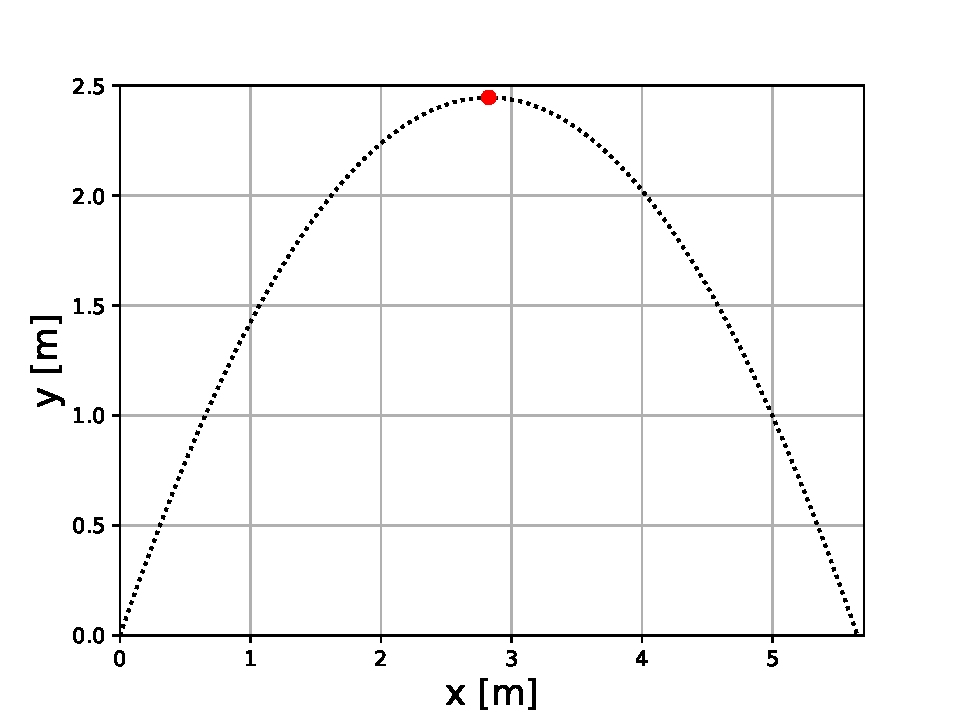
\includegraphics[scale=0.55]{traiettoria.pdf}
\caption{Traiettoria parabolica
percorsa dalla pallina ($|v_0|=8$ m/s).\label{fig:traiettoria} }
\end{figure}

Per ricavare $t_f$ basta uguagliare la gittata $d$ a $x(t_f)$:
%
\begin{equation*}
\frac{\sqrt{3}|v_0|^2}{2g}=\frac{|v_0|}{2}t_f \quad \Rightarrow \quad t_f=\frac{\sqrt{3}|v_0|}{g}
\end{equation*}
%
Le componenti di $\vec{v_1}$ saranno allora:
%
\begin{gather*}
(v_1)_x=(v_0)_x= \frac{|v_0|}{2}\\
(v_1)_y=(v_0)_y - g t_f= \frac{|v_0|\sqrt{3}}{2} - \sqrt{3}|v_0| = - \frac{|v_0|\sqrt{3}}{2}
\end{gather*}
%
Notiamo che $|\vec{v_1}|=|\vec{v_0}|$. 

\subsection{Moto uniformemente accelerato bis \rstar}
Una particella si muove su un piano cartesiano con accelerazione costante e pari a:
%
\begin{gather*}
\vec{a}=a\big(\frac{1}{\sqrt{2}},\frac{1}{\sqrt{2}}\big)
\end{gather*}
%
Che angolo forma l'accelerazione con l'asse delle $x$? Sapendo che al tempo $t_0=0$ la velocità della particella è $\vec{v_0}=(v_0,0)$ e la sua posizione $\vec{r_0}=(0,\frac{d}{2})$, scrivere la legge oraria $\vec{r}(t)$, scomponendola poi nelle due componenti. In quale istante di tempo $t_1$ la particella attraversa la retta descritta dall'equazione $y(x)=-x+2d$? Qual è il suo vettore velocità in questo istante? Che angolo forma con la velocità iniziale $\vec{v_0}$? Che angolo forma il vettore \textit{variazione di velocità} fra gli istanti $t_1$ e $t_0$ con $\vec{v_0}$? Trovare i risultati numerici per $v_0=1 \frac{\text{m}}{\text{s}}$, $d=2$ m e $a=g/4$ con $g$ l'accelerazione di gravità ($g\simeq9.81 \frac{\text{m}}{\text{s}^2}$).

\subsubsection*{Soluzione}
Il vettore $\vec{a}$ forma un angolo $\alpha=\arctan(\frac{a_y}{a_x})=\arctan(1)=\frac{\pi}{4}= 45^\circ$ con l'asse delle $x$. Il moto della particella è uniformemente accelerato e quindi la sua legge oraria si scrive: 
%
\begin{gather*}
\vec{r}(t)=\frac{1}{2}\vec{a}t^2 +\vec{v_0} t + \vec{r_0}
\end{gather*}
%
Che scomposta in componenti diventa: 
%
\begin{gather*}
x(t)=\frac{1}{2\sqrt{2}}at^2 + v_0 t \\
y(t)=\frac{1}{2\sqrt{2}}at^2  + \frac{d}{2}
\end{gather*}
%
All'istante di tempo $t_1$ in cui la particella attraversa la retta $y(x)=-x+2d$ si ha, uguagliando la coordinata y al tempo $t_1$ per la retta e per la legge oraria:
%
\begin{gather*}
y(t_1)=-x(t_1)+2d \quad \Rightarrow \quad \frac{1}{2\sqrt{2}}at_1^2  +  \frac{d}{2} = -\frac{1}{2\sqrt{2}}at_1^2 - v_0 t_1+2d
\end{gather*}
%
Si ottiene quindi un'equazione di secondo grado per $t_1$:
%
\begin{gather*}
\frac{1}{\sqrt{2}}at_1^2  + v_0 t_1 - \frac{3}{2}d =0
\end{gather*} 
%
Le due soluzioni sono:
%
\begin{gather*}
\frac{1}{\sqrt{2}a}\bigg(-v_0\pm \sqrt{v_0^2+3\sqrt{2}ad}\bigg)
\end{gather*} 
%
Solo la soluzione col $+$ è positiva, per cui è quella che ci interessa. Con i valori numerici indicati nel testo si ottiene: 
%
\begin{gather*}
t_1\simeq 1.06 \; \;\text{s}
\end{gather*} 
%
La velocità della particella a un generico istante $t$ è: 
%
\begin{gather*}
\vec{v}(t)=\vec{v}_0 + \vec{a}t
\end{gather*} 
%
che in componenti diventa:
%
\begin{gather*}
v_x(t)=v_0 + \frac{a}{\sqrt{2}}t\\
v_y(t)=\frac{a}{\sqrt{2}}t
\end{gather*} 
%
L'angolo che questo vettore forma con l'asse delle $x$, e quindi con la velocità iniziale è $\vec{v}_0$, è: 
%
\begin{gather*}
\theta=\arctan\big(\frac{\frac{a}{\sqrt{2}}t}{v_0 + \frac{a}{\sqrt{2}}t} \big)
\end{gather*} 
%
Sostituendo $t=t_1$ si trova:
%
\begin{gather*}
\theta \approx 33^\circ
\end{gather*} 
%
La variazione di velocità è $\Delta \vec{v}=\vec{v}(t)-\vec{v}_0=\vec{a}t$ o in componenti:
%
\begin{gather*}
\Delta v_x(t)=\frac{a}{\sqrt{2}}t\\
\Delta v_y(t)=\frac{a}{\sqrt{2}}t
\end{gather*} 
%
che è un vettore inclinato di $\frac{\pi}{4}=45^\circ$ rispetto all'origine. La retta, la traiettoria della particella e i vettori velocità 
$\vec{v_0}$ e $\vec{v}(t_1)$ sono rappresentati in Figura \ref{fig:particella}. 

 \begin{figure}[!ht]
 \centering
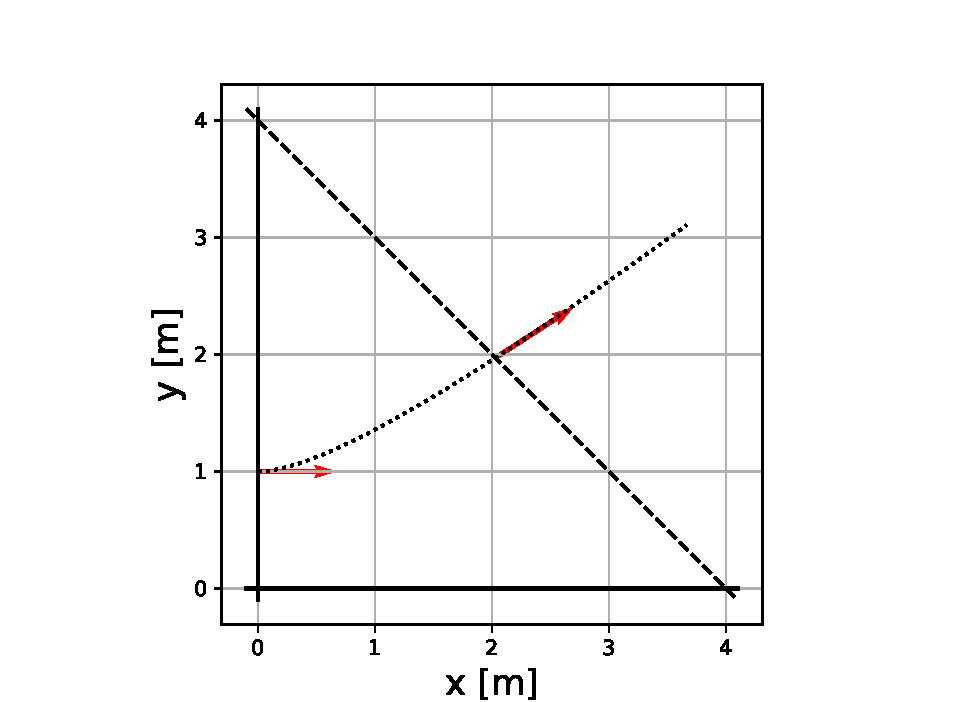
\includegraphics[scale=0.65]{particella.pdf}
\caption{Retta $y=-x+2d$, la traiettoria della particella e i vettori velocità $\vec{v_0}$ e $\vec{v}(t_1)$ (la lunghezza dei vettori in figura è puramente indicativa). I valori numerici utilizzati per $a$, $d$, $v_0$ sono quelli indicati nel testo.  \label{fig:particella} }
\end{figure}

\subsection{Lancio di un sasso \rstar}
Una pietra viene lanciata verticalmente \textit{verso l'alto}, con una velocità iniziale di $12.0$ m/s, dal bordo di uno strapiombo alto $70 $ m.
(a) Dopo quanto tempo raggiungerà la base dello strapiombo?
(b) Quale sarà la sua velocità appena prima di colpire il suolo?
(c) Quale sarà la distanza totale percorsa al momento dell'impatto?

\subsubsection*{Soluzione}
La pietra si muove di moto uniformemente accelerato lungo l'asse $y$ (nel sistema cartesiano in cui $\vec{g}=-g\hat{y}$). Detta $v_0=+12.0$ m/s la velocità iniziale della pietra, la legge oraria del corpo è:
\begin{equation*}
y(t)=h+v_0t - \frac{1}{2} gt^2 
\end{equation*}
a) Il tempo $t_f$ in cui la pietra raggiunge la base dello strapiombo
si trova imponendo che la coordinata $y$ della pietra sia $0$ al tempo $t_f$, quindi: $y(t_f)=0$. Si ha allora: 
\begin{equation*}
\frac{1}{2} gt_f^2 -v_0 t_f - h= 0 \quad \Rightarrow \quad t_f=\frac{v_0 + \sqrt{v_0^2+2hg}}{g}
\end{equation*}
Si è risolta l'equazione di secondo grado per $t_f$ prendendo l'unica soluzione fisica, quella con $t_f>0$ ovvero con il segno $+$. Inserendo i valori numerici si ottiene:
\begin{equation*}
t_f \simeq 5.19 \text{s}
\end{equation*}

b) La velocità $v_y(t)$ della pietra al tempo generico $t$ si scrive:
\begin{equation*}
v_y(t)=v_0 - gt 
\end{equation*}
La velocità un'istante prima dell'impatto a terra si ottiene ponendo $t=t_f$, con $t_f$ ricavato prima:
\begin{equation*}
v_y(t_f)=-\sqrt{v_0^2+2hg} \simeq - 39 \frac{\text{m}}{\text{s}}
\end{equation*}

c) Per trovare la distanza percorsa in totale bisogna dapprima
trovare l'altezza massima $y_{max}$ raggiunta dalla pietra. Detto $t^*$ l'istante di tempo in cui la pietra raggiunge l'altezza massima, si deve avere $v_y(t^*)=0$. Allora:
\begin{equation*}
t^*=\frac{v_0}{g} \quad \Rightarrow \quad y_{max}=y(t^*)=h+\frac{v_0^2}{g} - \frac{1}{2} \frac{v_0^2}{g} = h+\frac{1}{2} \frac{v_0^2}{g}
\end{equation*}
La distanza totale percorsa dalla pietra sarà $y_{max}-h$ (tratto in salita) \text{più} $y_{max}$ e quindi:
\begin{equation*}
d=(y_{max}-h)+y_{max}=2y_{max}- h = h+\frac{v_0^2}{g} \simeq 85 \text{m}
\end{equation*}


\subsection{Moto di un razzo \rstar}
Un razzo sale verticalmente, partendo da fermo, con un'accelerazione $a_{0}=3.2 \; \text{m/s}^2$ finché finisce il carburante a $h_{1}=1200\;\text{m}$ di altezza. Dopo questo punto, la sua accelerazione è quella di gravità, verso il basso.
\begin{enumerate}[label=\alph*)]
\item  Qual è la velocità del razzo nel momento in cui finisce il carburante?
\item Quanto tempo impiega a raggiungere quel punto?
\item Quale altezza massima raggiunge il razzo?
\item Quanto tempo occorre per raggiungere la massima altezza?
\item Con quale velocità il razzo colpisce la Terra?
\item Per quanto tempo totale il razzo rimane in aria?
\end{enumerate}


\subsubsection*{Soluzione}
I primi due punti si risolvono subito utilizzando le note leggi del moto uniformemente accelerato: 
\begin{equation*}
a) \qquad v_{1}=\sqrt{2a_{0}h_{1}}=88 \; \frac{\text{m}}{\text{s}}
\end{equation*}
\begin{equation*}
b)\qquad  t_{1}=\frac{v_{1}}{a_{0}}=27 \; \text{s}
\end{equation*}
Il tratto aggiuntivo percorso dal razzo dopo la fine del carburante, prima che la (de)celerazione $-g$ riesca a fermarlo è:
\begin{equation*}
h_{2}=\frac{v_{1}^2}{2g}=395 \;\text{m}
\end{equation*}
quindi l'altezza massima raggiunta sarà:
\begin{equation*}
c) \qquad h_{max}=h_{1}+h_{2}=1595 \; \text{m}
\end{equation*}
e il tempo impiegato per raggiungerla:
\begin{equation*}
d) \qquad t_{2}=t_{1}+\sqrt{\frac{2h_{2}}{g}}= 36 \; \text{s}
\end{equation*}
Per schiantarsi a terra il razzo dovrà poi cadere partendo dall'altezza massima (quindi con una velocità iniziale nulla) sotto l'effetto dell'accelerazione di gravità. Quindi:
\begin{equation*}
e) \qquad  v_{impatto}=-\sqrt{2gh_{max}}=-177 \; \frac{\text{m}}{\text{s}}
\end{equation*}
E infine $t_{tot}=t_{2}+t_{caduta}$, dove $t_{caduta}$ è il tempo necessario affichè il razzo si schianti a terra dopo aver raggiunto l'altezza massima:
\begin{equation*}
f)\qquad  t_{tot}=t_{2}+\sqrt{\frac{2h_{max}}{g}}=(36+18)s=54\;\text{s}.
\end{equation*}


\subsection{Attraversare un fiume \rstar\rstar}
Una barchetta, la cui velocità in acqua ferma è $v_b$, deve attraversare un fiume largo $l_y$ e risalire il fiume di $l_x$. Per fare ciò il pilota dirige la barca controcorrente con un angolo di $45\degree$. Quale è la velocità della corrente del fiume? Risolvere per: $v_b=2\;\text{m/s}$, $l_y=260\;\text{m}$, $l_x=130\;\text{m}$. La situazione è schematizzata in Figura \ref{fig:river}.

\begin{figure}[!ht]
 \centering
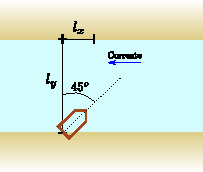
\includegraphics[scale=2]{river.pdf}
\caption{Barchetta che attraversa il fiume.  \label{fig:river} }
\end{figure}

\subsubsection*{Soluzione}
Siamo di fronte ad un problema in cui compaiono velocità relative, la relazione che lega i sistemi di riferimento è:
%
\begin{gather*}
\vec{v}=\vec{v}_{O'}+\vec{v}'
\end{gather*}
%
Per sfruttare il dato del problema sulla velocità della barchetta in acqua ferma definiamo O' il sistema di riferimento solidale con la corrente $\vec{v}_{O'}=\vec{v}_{c}$ mentre $\vec{v}'=\vec{v}_b$. Abbiamo dunque nel sistema di riferimento solidale con la sponda:
%
\begin{gather*}
\vec{v}=(-v_c+v_{bx})\hat{x}+v_{by}\hat{y}=(-v_c+\frac{\sqrt{2}}{2}v_{b})\hat{x}+\frac{\sqrt{2}}{2}v_{b}\hat{y}
\end{gather*}
%
Ora dobbiamo determinare per quanto tempo la barca naviga nel fiume, questo equivale a capire il tempo che la barca impiega per raggiungere la sponda opposta nel fiume, dunque:
%
\begin{gather*}
v_{by}=\frac{l_y}{t^*} \Rightarrow t^*=\frac{2}{\sqrt{2}}\frac{l_y}{v_b}=\sqrt{2}\frac{l_y}{v_b}
\end{gather*}
%
Adesso, conoscendo la distanza del fiume che si vuole risalire ed il tempo di percorrenza, ricaviamo quale deve essere la velocità orizzontale della corrente:
%
\begin{gather*}
l_x=(-v_c+\frac{\sqrt{2}}{2}v_{b})\cdot t^* \Rightarrow v_c=\frac{\sqrt{2}}{2}v_b -\frac{l_x}{t^*}=\frac{\sqrt{2}}{2}v_b -\frac{1}{\sqrt{2}}\frac{l_x}{l_y}v_b
\end{gather*}
%
Con i valori numerici si ottiene $v_c=\sqrt{2}/2\;\text{m/s} \approx 0.71 \;\text{m/s}$.

\subsection{Passaggio a livello \rstar}
Un uomo si trova nella sua automobile, lungo un viale rettilineo. Sulla mappa della città il viale è individuato 
dall'equazione: $y(x)=-x/\sqrt{3}$. All'istante $t_0=0$ l'uomo si trova nel punto $P=d (\frac{\sqrt{3}}{2}, -\frac{1}{2})$, con $d=500$ m. In questo stesso istante egli inizia a muoversi con accelerazione costante $a$ diretta lungo il versore $(-\frac{\sqrt{3}}{2}, +\frac{1}{2})$. Nel punto $O$ origine del sistema di riferimento cartesiano, il viale incrocia perpendicolarmente una ferrovia, anch'essa descrivibile come una retta. Scriverne l'equazione. Scrivere le componenti del vettore velocità $\vec{v}$ di un treno che si muove di moto rettilineo uniforme lungo la ferrovia, puntando nella direzione degli $x$ positivi. Supponiamo che $|\vec{v}|=100$ km/h.  Quanto vale $|\vec{v}|$ in m/s?  All'istante $t_0$ la locomotiva del treno si trova a distanza $4d$ da $O$ e ha coordinata $x$ negativa. Scrivere le coordinate della sua posizione $Q$. Se il passaggio a livello si chiude quando il treno è a distanza $2d$ dall'origine, quale dev'essere al minimo l'accelerazione $a$ dell'automobilista se egli vuole passare \textit{prima} che il passaggio a livello si chiuda? Per questo valore di $a$ scrivere le componenti del vettore velocità \textit{relativa} fra treno e automobile nell'istante in cui questa passa per $O$.
\subsubsection*{Soluzione}
Data una retta passante per l'origine $y=ax$, la retta a essa perpendicolare 
è $y=-\frac{1}{a}x$. Nel nostro caso $a=-\frac{1}{\sqrt{3}}$ e quindi
la retta che descrive la ferrovia sulla mappa della città è: $y=\sqrt{3}x$. Il versore $\hat{e}$ appartenente a questa retta e diretto verso gli $x$ positivi è: $\hat{e}=\big(\frac{1}{2}, \frac{\sqrt{3}}{2} \big)$, quindi
il vettore velocità del treno è a ogni istante:
%
\begin{equation*}
\vec{v}=|\vec{v}|\big(\frac{1}{2}, \frac{\sqrt{3}}{2} \big)
\end{equation*}
%
Si ha: 
%
\begin{equation*}
|\vec{v}|=100 \frac{\text{km}}{\text{h}}= 100 \frac{10^3 \text{  m}}{3.6 \cdot 10^3 \text{  s}}= \frac{100}{3.6} \frac{\text{m}}{\text{s}} \approx 27.78 \frac{\text{m}}{\text{s}}
\end{equation*}
%
Il punto $Q$ corrisponde a un vettore posizione diretto lungo $-\hat{e}$ e di modulo $4d$, quindi:
%
\begin{equation*}
Q=4d\big(-\frac{1}{2}, -\frac{\sqrt{3}}{2} \big)
\end{equation*}
%
La situazione è rappresentata in Figura \ref{fig:cartina}. 

 \begin{figure}[!ht]
 \centering
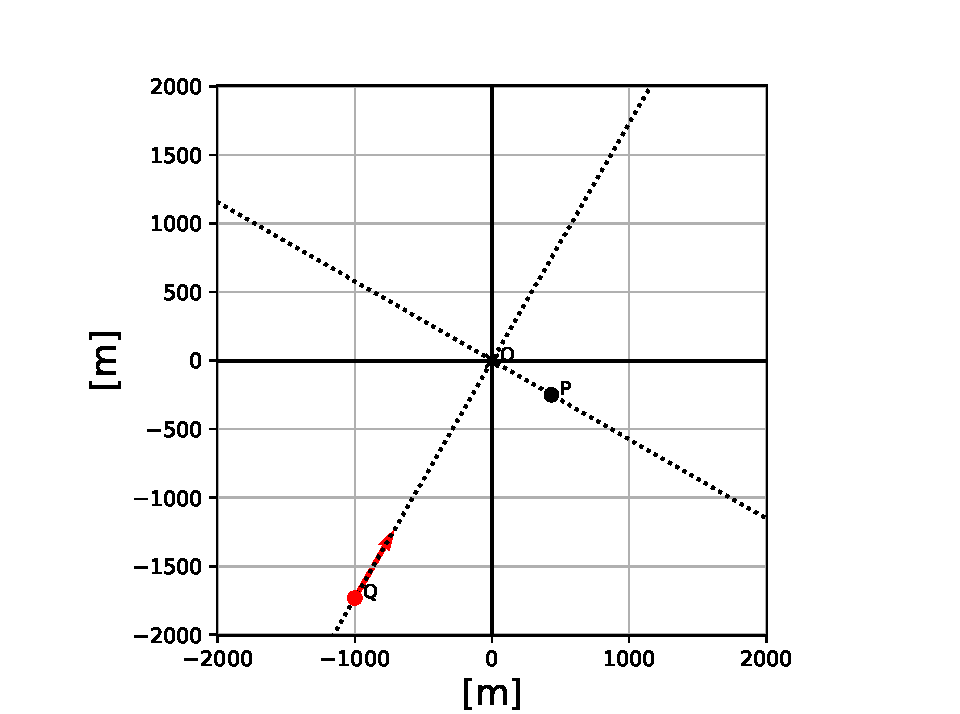
\includegraphics[scale=0.55]{cartina.pdf}
\caption{Mappa della città con la ferrovia, il viale e i punti $P$, $Q$ e $O$ (scala realistica per $d=500$ m). E' raffigurato anche il vettore velocità del treno.\label{fig:cartina} }
\end{figure}

L'automobilista si muove di moto uniformemente accelerato, con accelerazione $a$. L'istante di tempo $t_1$ in cui l'automobilista arriva a $O$ si trova ponendo $\frac{1}{2}at_1^2$ uguale allo spostamento $d$, quindi:
%
\begin{equation*}
t_1=\sqrt{\frac{2d}{a}}
\end{equation*}
%
L'istante di tempo $t_2$ in cui il treno arriva a distanza $2d$ da $O$ (cioè quando si chiude il passaggio a livello) è:
%
\begin{equation*}
t_2=\frac{2d}{|\vec{v}|}
\end{equation*}
%
La condizione che vogliamo che si realizzi è $t_2>t_1$, quindi:
%
\begin{equation*}
\frac{2d}{|\vec{v}|}>\sqrt{\frac{2d}{a}}
\end{equation*}
%
Prendendo il quadrato da entrambe le parti (N.B. si tratta di due quantità positive) si trova:
%
\begin{equation*}
a>a_{min}=\frac{|\vec{v}|^2}{2d}
\end{equation*}
%
Per i valori numerici considerati: $a_{min}\simeq 0.77$ m/s$^2$. Se $a=a_{min}$ allora nel momento in cui raggiunge $O$, l'automobile ha una velocità (in modulo):
%
\begin{equation*}
V=at_1=\frac{|\vec{v}|^2}{2d}\frac{2d}{|\vec{v}|}=|\vec{v}|
\end{equation*}
%
Il suo vettore velocità è allora:
%
\begin{equation*}
\vec{V}=|\vec{v}| \big(-\frac{\sqrt{3}}{2}, +\frac{1}{2}\big)
\end{equation*}
%
(si è considerato il versore $\big(-\frac{\sqrt{3}}{2}, +\frac{1}{2}\big)$
appartente alla retta $y(x)=-x/\sqrt{3}$).  Il vettore velocità relativa si ottiene sottraendo il vettore velocità del treno:
%
\begin{equation*}
\vec{V} - \vec{v}=|\vec{v}| \big(-\frac{\sqrt{3}}{2} - \frac{1}{2}, +\frac{1}{2} - \frac{\sqrt{3}}{2}\big)
\end{equation*}
%
\subsection{Passaggio a livello (seconda parte) \rstar\rstar}
Nella situazione dell'esercizio precedente si trovi la distanza $D$ tra la locomotiva e l'automobile ad un istante di tempo $t$ generico ($t>t_0=0$), ricavando così la funzione $D(t)$. Si determini poi a quale $t=\bar{t}$ la distanza è minima. Per facilitare i calcoli si introducano i parametri \textit{adimensionali}:
%
\begin{equation*}
f(t)=\frac{D^2(t)}{d^2}\quad \quad\alpha=\frac{a}{a_{min}}\quad \quad \tau=t\frac{v}{d}
\end{equation*}
%
e si consideri il caso particolare in cui $\alpha=2$.  \textit{Suggerimento}: si svolgano i conti nel miglior sistema di riferimento possibile...


\subsubsection*{Soluzione}
Conviene utilizzare un sistema di riferimento $S'$ che abbia come assi cartesiani i due versori:
%
\begin{equation*}
\hat{e}_1=\big(\frac{1}{2}, \frac{\sqrt{3}}{2}\big) \qquad \hat{e}_2=\big(-\frac{\sqrt{3}}{2}, \frac{1}{2}\big)
\end{equation*}
%
$S'$ si ottiene operando una rotazione di $60^\circ$ (in senso antiorario) del sistema di partenza $S$. Quindi un punto di coordinate $(x,y)$ in $S$ ha coordinate:
%
\begin{gather*}
(\frac{1}{2}x+\frac{\sqrt{3}}{2}y, -\frac{\sqrt{3}}{2}x+\frac{1}{2}y )
\end{gather*}
%
in $S'$ (Figura \ref{fig:sistema2}).  

\begin{figure}[!ht]
 \centering
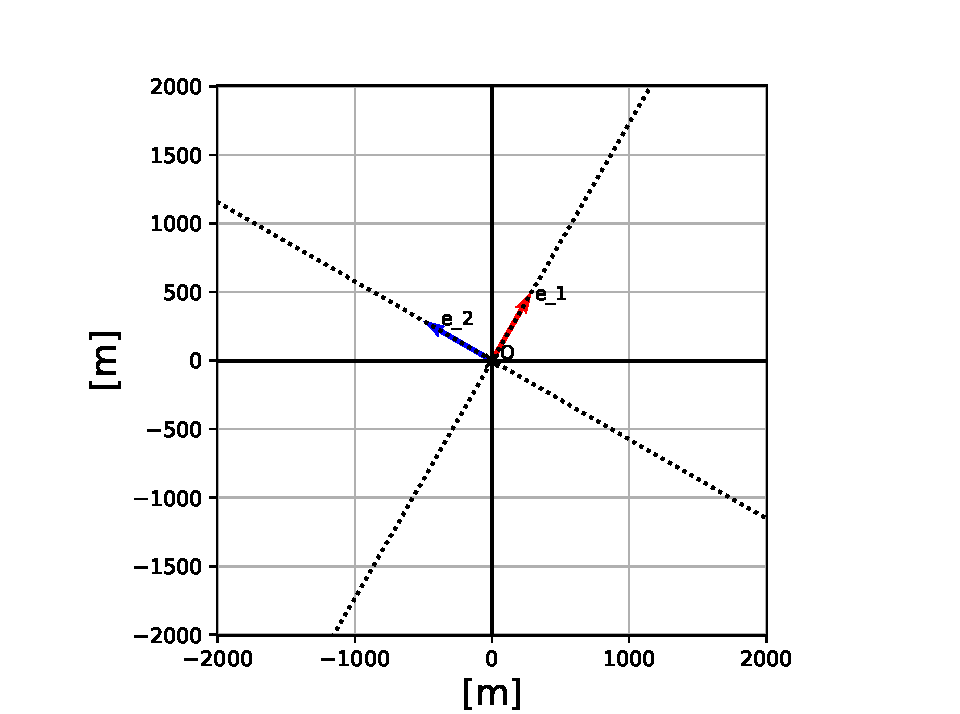
\includegraphics[scale=0.55]{sistema2.pdf}
\caption{Sistema di riferimento $S'$ dato dai versori $\hat{e}_1$ e $\hat{e}_2$. \label{fig:sistema2} }
\end{figure}


Le coordinate di $Q$ e $P$ diventano allora:
%
\begin{equation*}
Q=4d(-\frac{1}{4}-\frac{3}{4}, +\frac{\sqrt{3}}{4}-\frac{\sqrt{3}}{4})=4d(-1,0) \qquad P=d(\frac{\sqrt{3}}{4}-\frac{\sqrt{3}}{4}, -\frac{3}{4}-\frac{1}{4})=d(0,-1)
\end{equation*}
%
in $S'$, come del resto si poteva dedurre facilmente dal disegno. Le leggi orarie di treno e automobile sono allora rispettivamente:
%
\begin{gather*}
\vec{r}_T(t)=(-4d+vt,0)  \\
\vec{r}_A(t)=(0,\frac{1}{2}at^2 -d) 
\end{gather*}
%
$v$ corrisponde a $|\vec{v}|$ dell'esercizio precedente. $\vec{r}_T(t)$ e $\vec{r}_A(t)$ sono i vettori posizione 
in $S'$ a un istante generico di tempo $t>0$. La distanza tra i due oggetti è: $D(t)=|\vec{r}_T(t) - \vec{r}_A(t)|=|(-4d+vt, -\frac{1}{2}at^2 +d)|$, e quindi, ricordando la definizione di modulo di un vettore:
%
\begin{gather*}
D(t)=\sqrt{(-4d+vt)^2 + (d-\frac{1}{2}at^2)^2} =\sqrt{16d^2 -8dvt +v^2t^2 + d^2 - dat^2+\frac{1}{4}a^2t^4} = \\
=\sqrt{\frac{1}{4}a^2t^4+t^2(v^2-da)-8dvt+17d^2}\\
\end{gather*}
%
Conviene dividere tutto per $d$ ed elevare al quadrato, ottenendo così $f(t)$ come definita nel testo:
%
\begin{gather*}
f(t)=\frac{1}{4}\frac{a^2}{d^2}t^4+t^2\frac{v^2}{d^2}\big(1-\frac{ad}{v^2}\big)-8\frac{v}{d}t+17\\
\end{gather*}
%
Possiamo introdurre $a_{min}=\frac{v^2}{2d}$ dividendo e moltiplicando per questa quantità:
%
\begin{gather*}
f(t)=\frac{1}{4}\frac{a^2}{a_{min}^2}\frac{a_{min}^2}{d^2}t^4+t^2\frac{v^2}{d^2}\big(1-\frac{d}{v^2}\frac{a}{a_{min}}a_{min}\big)-8\frac{v}{d}t+17\\
\end{gather*}
%
Infine sostituendo la definizione di $a_{min}$:
%
\begin{gather*}
f(t)=\frac{1}{16}\alpha^2 \big(\frac{v}{d}t\big)^4+(1-\frac{1}{2}\alpha)\big(\frac{v}{d}t\big)^2-8\big(\frac{v}{d}t\big)+17\\
\end{gather*}
%
e quindi:
%
\begin{gather*}
f(\tau)=\frac{1}{16}\alpha^2 \tau^4+(1-\frac{1}{2}\alpha)\tau^2-8\tau+17
\end{gather*}
%
Quello che dobbiamo fare è trovare il minimo di questa funzione rispetto a $t$, oppure rispetto a $\tau$ (è la stessa cosa, sono proporzionali). Per farlo calcoliamo la derivata e imponiamola uguale a $0$:
%
\begin{gather*}
f'(\bar{\tau})=0 \quad \Rightarrow \quad \frac{1}{4}\alpha^2 \bar{\tau}^3+(2-\alpha)\bar{\tau}=8 \qquad \qquad \bar{\tau}=\bar{t}\frac{v}{d}
\end{gather*}
%
Questa è un'equazione di terzo grado, non facile da risolvere. 
Ma ponendo $\alpha=2$ come consigliato nel testo troviamo:
%
\begin{gather*}
\bar{\tau}^3=8 \quad \Rightarrow \quad  \bar{\tau}=2 \quad \Rightarrow \quad  \bar{t}=\frac{2d}{v}
\end{gather*}
%
In questo istante la distanza tra treno e automobile vale: 
%
\begin{gather*}
D(t)=\sqrt{\frac{1}{4}a^2 \frac{16d^4}{v^4}-8dv\frac{2d}{v}+17d^2}=\sqrt{4d^2-16d^2+17d^2}=\sqrt{4d^2-16d^2+17d^2}=d\sqrt{5}\\
\end{gather*}
%
In \ref{fig:distanza} sono riportati i grafici di $D(\tau)=f^2(\tau)d^2$ per differenti valori di $a$, cioè di $\alpha$ : $\alpha=0$ (linea azzurra), $\alpha=1$ (linea arancione), $\alpha=2$ (linea verde). La linea tratteggiata corrisponde a $\frac{D}{d}=\sqrt{5}$, che, come abbiamo visto, è la distanza minima per $\alpha=2$ (infatti è la tangente alla linea verde). Notare che $D(\tau=0)=D(t=0)$
è uguale in tutti i casi (perché indipendentemente da $a$ all'istante di tempo iniziale la distanza tra treno e automobile è $D(t=0)=\sqrt{(4d)^2+d^2}=d\sqrt{17}\simeq 4.12 d$).  
 \begin{figure}[!ht]
 \centering
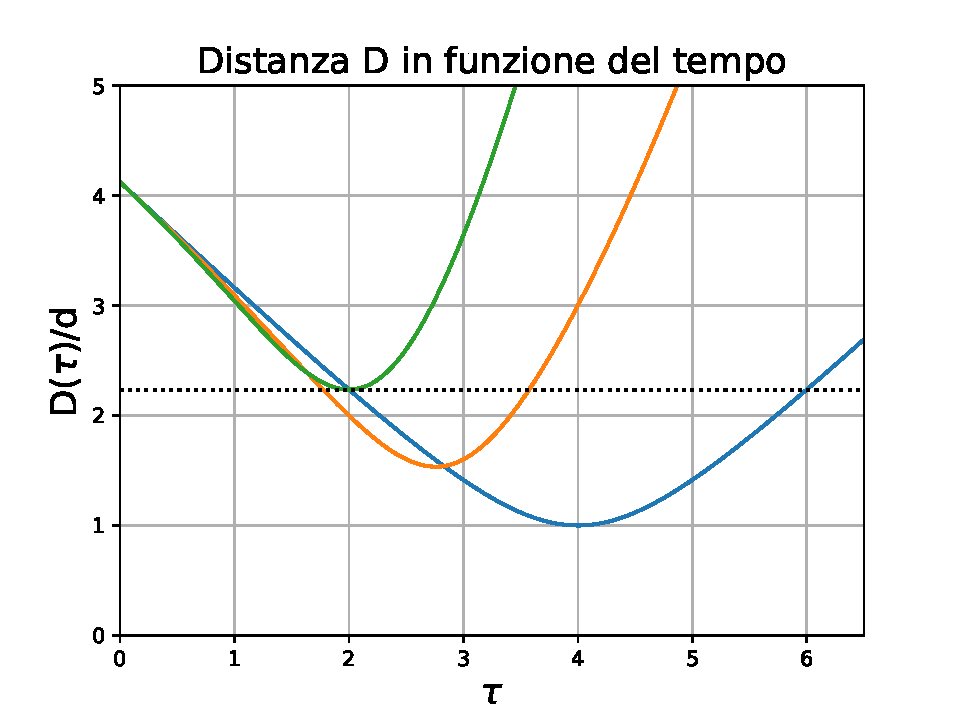
\includegraphics[scale=0.55]{distanza.pdf}
\caption{Funzione $D(\tau)$ per diversi $\alpha$. Il caso studiato nell'esercizio è rappresentato dalla linea verde. \label{fig:distanza} }
\end{figure}

\subsection{Lancio di un sasso da una collina \rstar\rstar}
Un ragazzo si trova in cima a una collina di pendenza $45^\circ$.
In un sistema di riferimento cartesiano posizionato alla 
base della collina la sua posizione è: $(0,h)$, mentre il profilo della collina è dato dalla retta:
%
\begin{equation*}
y=-x+h
\end{equation*} 
%
All'istante di tempo $t_0=0$ il ragazzo calcia
un sasso con velocità iniziale:
%
\begin{equation*}
\vec{v_0}=(v_0,0) \qquad v_0=15 \; \; \; \text{m/s}
\end{equation*} 
%
In che istante di tempo $t_1$ il sasso incontra di nuovo la collina?

\subsubsection*{Soluzione}
Il sasso si muove di moto uniformemente accelerato lungo $\hat{y}$, con accelerazione uguale a quella di gravità: $\vec{g}=-g \hat{y}$. Lungo $\hat{x}$ il moto invece è rettilineo uniforme. La legge oraria del sasso è quindi: 
%
\begin{gather*}
x(t)= v_0 t \\
y(t)= h - \frac{1}{2} g t^2
\end{gather*} 
%
Al tempo $t_1$ (nostra incognita), il sasso si trova di nuovo 
lungo il profilo della collina, per cui:
%
\begin{gather*}
y(t_1)=h- x(t_1) \quad \Rightarrow \quad h - \frac{1}{2} g t_1^2=h- v_0 t_1
\end{gather*} 
%
Ricaviamo quindi:
%
\begin{gather*}
 \frac{1}{2} g t_1^2= v_0 t_1  \quad \Rightarrow \quad t_1= \frac{2 v_0}{g}
\end{gather*} 
%
Inserendo i valori numerici si ottiene: 
%
\begin{gather*}
t_1= \frac{2\cdot 15 \text{  m/s}}{9.81 \text{  m/s}^2} \simeq 3.06 \text{  s}
\end{gather*} 
%

\subsection{Canestro! \rstar\rstar\rstar} 
Un pallone da basket è lanciato da un'altezza iniziale $h=2.40$ m con velocità iniziale $|\vec{v_0}|=12$ m/s. 
In un sistema di riferimento cartesiano, la posizione iniziale del pallone è quindi: $(0,h)$. L'angolo $\theta$ fra il vettore $\vec{v_0}$ e il versore $\hat{x}$ è $35^\circ$. Il giocatore che lancia il pallone riesce a centrare un canestro posizionato nel punto $(d,H)$ con $H=3.05$ m.  Qual è la distanza $d$ del giocatore dal canestro? Con quale angolo rispetto a $\hat{x}$ la palla entra nel canestro? Si supponga che il pallone sia approssimatile come un punto materiale. 

\subsubsection*{Soluzione}
Il vettore velocità iniziale è:
%
\begin{equation*}
\vec{v_0}=|v_0| \big(\cos(\theta), \sin(\theta)\big)
\end{equation*}
%
Il pallone da basket si muove di moto uniformemente accelerato lungo $\hat{y}$, con accelerazione uguale a quella di gravità: $\vec{g}=-g \hat{y}$. Lungo $\hat{x}$ il moto invece è rettilineo uniforme. La legge oraria del pallone è quindi: 
%
\begin{gather*}
x(t)= |v_0| t \cos(\theta)\\
y(t)= h + |v_0| t \sin(\theta) - \frac{1}{2} g t^2
\end{gather*} 
%
La traiettoria descritta dal pallone è una parabola. Possiamo ricavarne l'equazione, scrivendo $t=\frac{x(t)}{|v_0|  \cos(\theta)}$ e sostituendo nell'equazione per $y(t)$. Si ottiene così: 
%
\begin{gather*}
y= h + \frac{\sin(\theta)}{\cos(\theta)} x - \frac{1}{2}  \frac{g}{|v_0|^2  \cos^2(\theta)}x^2
\end{gather*} 
%
Sappiamo che la traiettoria passa per il canestro, cioè per il punto $(d,H)$. Allora:
%
\begin{gather*}
H= h + \frac{\sin(\theta)}{\cos(\theta)} d - \frac{1}{2}  \frac{g}{|v_0|^2  \cos^2(\theta)}d^2
\end{gather*} 
%
Questa è un'equazione di secondo grado per l'incognita $d$. Le due soluzioni sono:
%
\begin{gather*}
\frac{|v_0|^2 \cos^2(\theta)}{g}\bigg[+\frac{\sin(\theta)}{\cos(\theta)} \pm \sqrt{\frac{\sin^2(\theta)}{\cos^2(\theta)} - \frac{2 g (H-h)}{|v_0|^2  \cos^2(\theta)} }\bigg] 
\end{gather*} 
%
Ci sono due soluzioni, entrambe positive. Questo perché la parabola passa due volte per l'altezza $H$: a sinistra e a destra del massimo in altezza (Figura \ref{fig:71}). Sono entrambe soluzioni accettabili,  tuttavia sembra più verosimile che il giocatore di basket faccia canestro sfruttando la seconda soluzione, quella con il segno $+$. Si ottiene quindi:
%
\begin{gather*}
d=\frac{|v_0|^2 \cos^2(\theta)}{g}\bigg[+\frac{\sin(\theta)}{\cos(\theta)} + \sqrt{\frac{\sin^2(\theta)}{\cos^2(\theta)} - \frac{2 g (H-h)}{|v_0|^2  \cos^2(\theta)} }\bigg] 
\end{gather*} 
%

Sostituendo i numeri valori dati nel testo: $d \simeq 12.8$ m.
 \begin{figure}[!ht]
 \centering
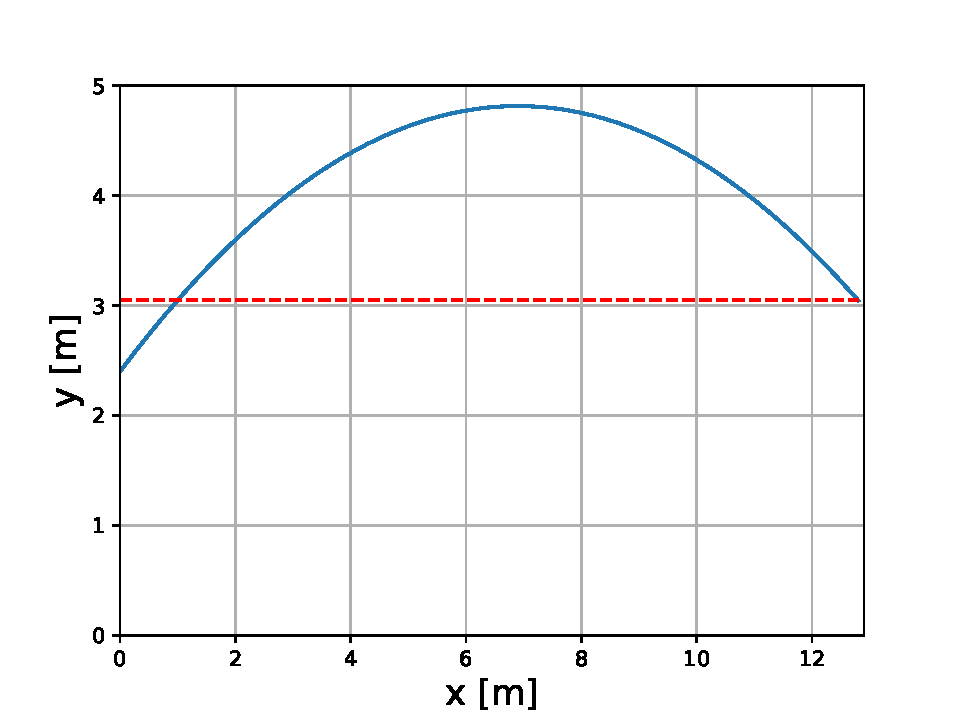
\includegraphics[scale=0.55]{71.pdf}
\caption{Traiettoria del pallone (linea continua). La linea tratteggiata indica l'altezza $H$ a cui si trova il canestro.\label{fig:71} }
\end{figure}
L'istante di tempo in cui il pallone entra nel canestro è: 
%
\begin{equation*}
t_f=\frac{d}{|v_0|  \cos(\theta)} \simeq 1.30 \text{  s}
\end{equation*}
%
La componente $x$ della velocità in questo momento è ovviamente $|v_0| \cos(\theta)$. La componente $y$ invece è:
%
\begin{equation*}
v_y(t_f)= |v_0|  \sin(\theta) - g t_f  \simeq - 5.88 \text{  m/s}
\end{equation*}
%
L'angolo con il quale il pallone entra nel canestro si trova 
considera
%
\begin{equation*}
\tan(\theta')=\frac{v_y(t_f)}{v_x(t_f)} \quad \Rightarrow \quad \theta' \simeq - 31^\circ
\end{equation*}
%

\subsection{Lancio doppio \rstar\rstar\rstar}
Un sasso $A$ è lasciato cadere da fermo dalla cima di un pozzo di altezza $h$ all'istante di tempo $t_0=0$. In quale istante di tempo $t_1$ esso tocca il fondo? A un certo istante di tempo $0<t_2<t_1$ viene lanciato 
un secondo sasso $B$, con velocità iniziale $\vec{v}=v \hat{y}$ (nel sistema di riferimento cartesiano in cui $\vec{g}=-g\hat{y}$ ). Come  dev'essere scelta la velocità $v$ affinché $B$ possa raggiungere $A$ prima che questo tocchi il fondo? Qual è il minimo valore del modulo di $v$ perché tale condizione sia realizzata? Calcolarne il valore numerico per $h=15$ m e $t_2=\frac{1}{2}t_1$. 

\subsubsection*{Soluzione}
La legge oraria del corpo $A$ è quella di un moto uniformemente accelerato lungo $\hat{y}$:
%
\begin{equation*}
y_A(t)=h- \frac{1}{2}g t^2
\end{equation*}
%
Quindi $A$ raggiunge il fondo all'istante $t_1= \sqrt{\frac{2h}{g}}$. 
La legge oraria di $B$ sarà:
%
\begin{equation*}
y_B(t)=h + v(t-t_2)- \frac{1}{2}g (t-t_2)^2 \qquad 0<t_2<\sqrt{\frac{2h}{g}}
\end{equation*}
%
La condizione che vogliamo che si verifichi è che $B$ raggiunga $A$ prima che questo tocchi il fondo. Questo significa che:
%
\begin{equation*}
y_B(\bar{t})=y_A(\bar{t}) 
\end{equation*}
%
per un qualche $\bar{t}$ appartenente all'intervallo $(t_2, t_1)$. La condizione diventa quindi:
%
\begin{equation*}
v(\bar{t}-t_2)- \frac{1}{2}g (\bar{t}-t_2)^2= - \frac{1}{2}g \bar{t}^2 \qquad t_2 < \bar{t} <t_1
\end{equation*}
%
Svolgendo il quadrato si ottiene:
%
\begin{equation*}
v(\bar{t}-t_2)- \frac{1}{2}g (-2\bar{t}t_2 + t_2^2)=0 \quad \Rightarrow \quad v=\frac{1}{2}g t_2\frac{t_2-2\bar{t}}{\bar{t}-t_2}
\end{equation*}
%
Occorre studiare $v$ come funzione di $\bar{t}$ nell'intervallo di interesse, ovvero $(t_2, t_1)$. In questo intervallo $v$ è sicuramente $<0$, perché  $\bar{t}>t_2$ e quindi $2\bar{t}>t_2$. Questo fatto ha un senso fisico intuitivo: il sasso $B$ deve essere lanciato con una certa velocità iniziale diretta verso il basso affinché possa raggiungere $A$, che ha già cominciato a cadere.  Per $\bar{t}\rightarrow t_2^+$ la funzione $v(\bar{t})$ diverge a $-\infty$. Per $\bar{t}\rightarrow t_1^-$ essa tende invece al valore :
%
\begin{equation*}
\frac{1}{2}g t_2\frac{t_2-2t_1}{t_1-t_2}
\end{equation*}
%
Nell'intervallo $(t_2, t_1)$ la funzione è crescente. In definitiva i valori
possibili di $v$ affinghé $B$ incontri $A$ a un $\bar{t}$ minore di $t_2$ e maggiore di $t_1$ sono:
%
\begin{equation*}
-\infty < v < - \frac{1}{2}g t_2\frac{2t_1-t_2}{t_1-t_2}
\end{equation*}
%
Il minimo valore del modulo di $v$ è quindi $|v_{min}|=\frac{1}{2}g t_2\frac{2t_1-t_2}{t_1-t_2}$. Se, come indicato nel testo $t_2=\frac{1}{2}t_1$, allora: 
%
\begin{equation*}
|v_{min}|=\frac{3}{4}g t_1= \frac{3}{4}\sqrt{2hg}
\end{equation*}
%
Per $h=15$ m si ottiene $|v_{min}| \approx 12.8$ m/s. In Figura  \ref{fig:sasso} sono rappresentate le leggi orarie $y_A(t)$ e $y_B(t)$ in questo caso, per $v=-|v_{min}|$ (linea tratteggiata) e per $v=-2|v_{min}|$ (linea continua).

 \begin{figure}[!ht]
 \centering
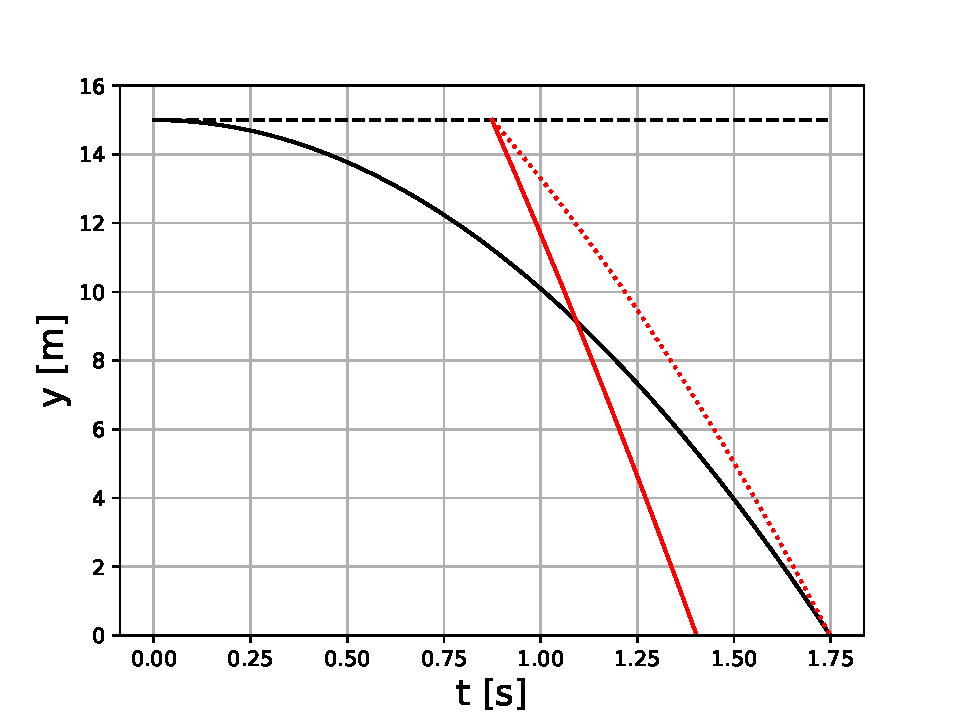
\includegraphics[scale=0.55]{sasso.pdf}
\caption{Legge oraria dei due sassi, per i valori numerici indicati nel testo e per due valori della velocità iniziale di $B$: $v=-|v_{min}|$ (linea tratteggiata) e $v=-2|v_{min}|$ (linea continua)}\label{fig:sasso} 
\end{figure}

\subsection{Moto delle lancette di un orologio \rstar}
Le lancette delle ore e dei minuti di un orologio da campanile sono lunghe rispettivamente $L_1=1$ m e $L_2=2$ m. Siano $P_1$ e $P_2$ le estremità esterne delle due lancette. Supponendo che esse si muovano in buona approssimazione di moto circolare uniforme ricavarne i periodi $T_1$ e $T_2$ e le frequenze
$f_1$ e $f_2$, espresse in Hz e in $\text{h}^{-1}$. Scrivere la legge oraria dei punti $P_1$ e $P_2$ in coordinate polari, misurando gli angoli $\phi_1$ e $\phi_2$ rispetto alla verticale (Figura \ref{fig:orologio1}) e misurando i tempi $t$ a partire dalle ore $12.00$. Scrivere anche i due vettori velocità $\vec{v_1}$, $\vec{v_2}$ (sempre in coordinate polari), ricavandone i moduli. Determinare infine a quali ore le lancette risulteranno perfettamente allineate. A quali ore invece saranno \textit{anti-allineate}?
 \begin{figure}[!ht]
 \centering
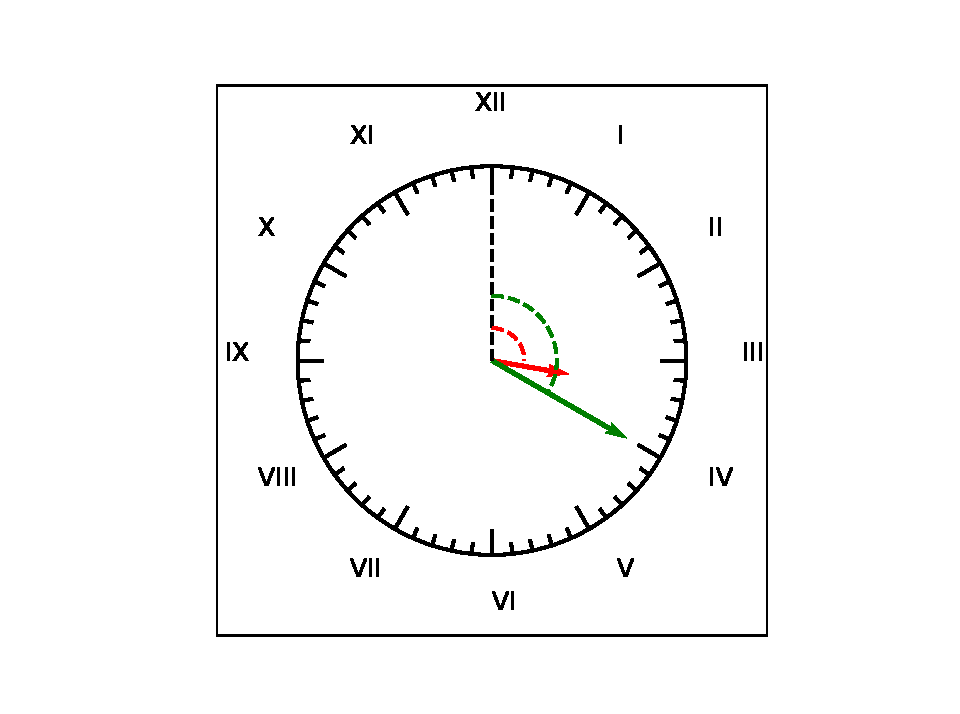
\includegraphics[scale=0.55]{orologio1.pdf}
\caption{Orologio e angoli di misura della posizione delle lancette nel sistema di coordinate polari piazzato nel centro dell'orologio (linea tratteggiata rossa=$\phi_1$, linea tratteggiata verde=$\phi_2$). \label{fig:orologio1} }
\end{figure}

\subsubsection*{Soluzione}
Se l'orologio funziona bene i periodi sono ovviamente:
%
\begin{equation*}
T_1=12 \; \; \text{h} \qquad \qquad T_2=1 \; \; \text{h}
\end{equation*}
%
Le frequenze sono:
%
\begin{gather*}
f_1=\frac{1}{T_1}\simeq 0.0833 \; \; \frac{1}{\text{h}}= 0.0833 \; \; \frac{1}{3600 \; \;  \text{s}} \simeq  2.314 \cdot 10^{-5} \text{s}^{-1}=2.314 \cdot 10^{-5} \text{Hz} \\
f_2=\frac{1}{T_2}\simeq 1 \; \; \frac{1}{\text{h}}= 1 \; \; \frac{1}{3600 \; \;  \text{s}} \simeq  2.778 \cdot 10^{-4} \text{s}^{-1}=2.778 \cdot 10^{-4}\text{Hz} 
\end{gather*}
%
In coordinate polari rispetto al centro dell'orologio il moto di $P_1$ e $P_2$ è assai semplice: i rispettivi raggi restano invariati, mentre gli angoli $\phi_1$ e $\phi_2$ crescono (linearmente col tempo). In altre parole
\begin{equation*}
 \left\{\begin{array}{lr}
  r_1(t)=L_1\\
  \phi_1(t)=2 \pi f_1 t \\
        \end{array}\right.
\qquad \qquad
 \left\{\begin{array}{lr}
  r_2(t)=L_2\\
  \phi_2(t)=2 \pi f_2 t \\
        \end{array}\right. 
\end{equation*}
Si è convenzionalmente posto l'istante iniziale $t=0$ alle ore $12.00$ (cioè quando $\phi_1=\phi_2=0$). I vettori velocità di $P_1$ e $P_2$ sono per ragioni geometriche
perpendicolari ai rispettivi raggi vettori, per cui le velocità sono parallele ai versori $\hat{\phi_1}, \hat{\phi_2}$. 
\begin{equation*}
 \left\{\begin{array}{lr}
 \vec{v_1}(t)= - v_1 \hat{\phi_1}(t) \qquad v_1= \frac{2 \pi L_1}{T_1} \simeq 1.4 \cdot 10^{-4} \frac{\text{m}}{\text{s}}\\
 \vec{v_2}(t)= - v_2 \hat{\phi_2}(t) \qquad v_2= \frac{2 \pi L_2}{T_2} \simeq 3.5 \cdot 10^{-3} \frac{\text{m}}{\text{s}}\\
        \end{array}\right.
\end{equation*}
Per ricavare i moduli $v_1, v_2$ si è notato ad esempio che $P_1$ si muove di una 
lunghezza totale $2\pi L_1$ (perimetro della circonferenza da esso tracciata) in un tempo $T_1$. I moduli delle velocità sono costanti per ipotesi (il moto è circolare uniforme). Si ha $v_2 =24  v_1=2\cdot 12 v_1$, perché: a) la lancetta dei minuti è due volte più lunga di quella delle ore; b) il tempo con cui essa effettua un giro è $12$ volte minore di quello che impiega la lancetta delle ore (quindi deve andare più veloce). Le lancette sono allineate quando $\phi_1$ e $\phi_2$ sono uguali \textit{a meno di un multiplo dell'angolo giro} $2\pi$ (infatti, come dovrebbe essere noto, gli angoli $0$, $2\pi$, $4\pi$ ... coincidono, cioè in coordinate polari $\phi$ \textit{è definito a meno di un multiplo di} $2\pi$). Quindi:
\begin{equation*}
\phi_2(t=t_n)=\phi_1(t=t_n)+ 2 \pi n \quad \Rightarrow \quad f_2 t_n=f_1 t_n+  n \quad \Rightarrow \quad t_n=\frac{n}{f_2 - f_1}
\end{equation*}
Notando che $f_2=12 f_1$: 
\begin{equation*}
t_n=\frac{n}{12f_1 - f_1}=\frac{n}{11f_1}=\frac{n}{11} T_1 =\frac{12}{11} n\; \; \text{h}
\end{equation*}
La prima volta che le lancette si allineano dopo le ore $12:00$ è al tempo:
\begin{equation*}
t_1=\frac{12}{11} \; \; \text{h} \simeq 1.090 \; \; \text{h}  
\end{equation*}
Attenzione: se vogliamo leggere i minuti, bisogna convertire in sessantesimi la parte di $t_1$ dopo il $.$, quindi:
\begin{equation*}
t_1\simeq 13 \; \; \text{h}  \; \;  5 \; \; \text{m} \; \; 27 \text{s}
\end{equation*}
dove abbiamo anche sommato $t_1$ al tempo iniziale, ovvero le $12.00$.  In questo istante l'orologio apparirà come in Figura \ref{fig:orologio2}.
 \begin{figure}[!ht]
 \centering
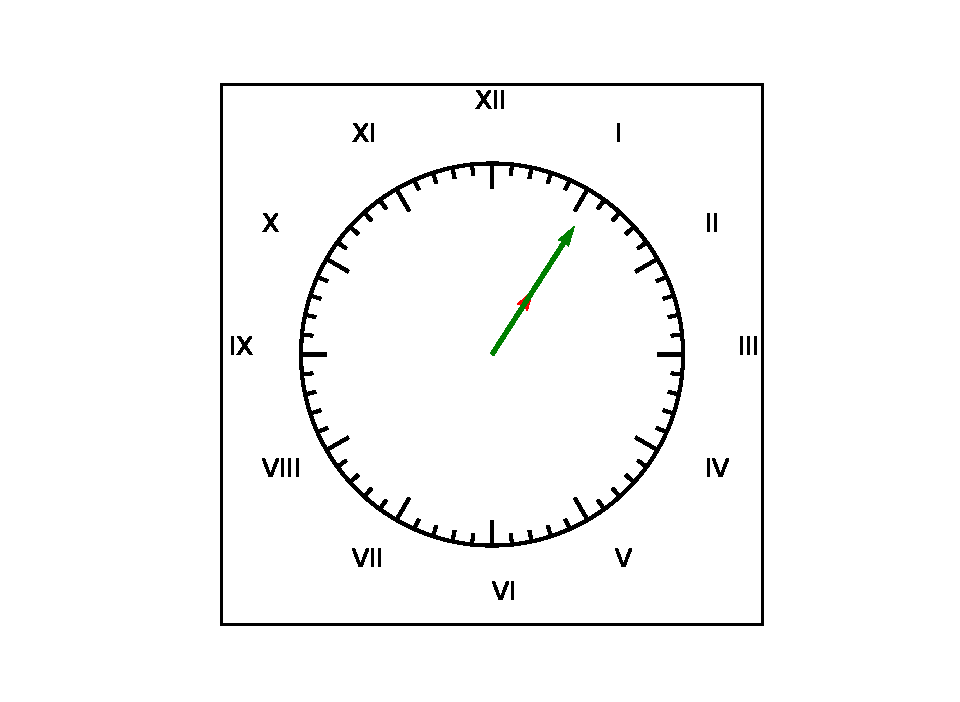
\includegraphics[scale=0.55]{orologio2.pdf}
\caption{Orologio al tempo $t_1$ (primo allineamento).  \label{fig:orologio2} }
\end{figure}

Il secondo allineamento avviene a: 
\begin{equation*}
t_2\simeq 14 \; \; \text{h}  \; \; 5 \; \; \text{m} \; \; 27 \text{s}
\end{equation*}
Per gli antiallineamenti la condizione è che $\phi_2=\phi_1+ 2\pi_n - \pi$, cioè:
\begin{equation*}
f_2 \overline{t}_n=f_1 \overline{t}_n+  n - \frac{1}{2}
\end{equation*}
da cui:
\begin{equation*}
\overline{t}_n=\frac{12}{11} (n - \frac{1}{2})\; \; \text{h}
\end{equation*}
Il primo antiallineamento avviene a: 
\begin{equation*}
\overline{t}_1=\frac{6}{11} \; \; \text{h} \simeq 0.545 \; \; \text{h}  
\end{equation*}
che corrisponde a:
\begin{equation*}
\overline{t}_1\simeq 12 \; \; \text{h}  \; \; 32 \; \; \text{m} \; \; 43 \text{s}
\end{equation*}
(Si veda Figura \ref{fig:orologio3}). 

 \begin{figure}[!ht]
 \centering
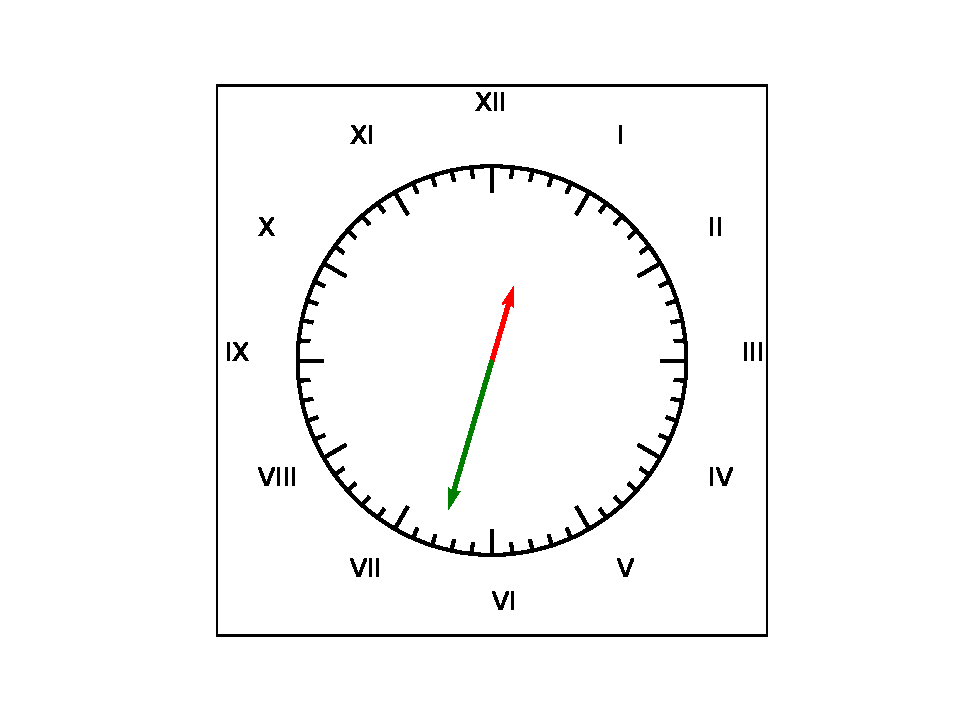
\includegraphics[scale=0.55]{orologio3.pdf}
\caption{Orologio al tempo $\overline{t}_1$ (primo anti-allineamento). \label{fig:orologio3} }
\end{figure}

\subsection{Moto circolare uniforme di una stazione spaziale \rstar\rstar} 
All'inizio del film \textit{2001: Odissea nello spazio} viene inquadrata una stazione spaziale costituita schematicamente da una circonferenza esterna collegata al suo centro da quattro bracci perpendicolari fra loro (Figura \ref{fig:ruota1}). In un opportuno piano cartesiano la circonferenza esterna, di raggio $R$, è centrata nell'origine $O$ del sistema stesso. La circonferenza e i quattro bracci ruotano attorno a $O$. Sia $P$ un punto materiale fissato sulla circonferenza esterna. Esso si muove, solidale alla circonferenza, di moto circolare uniforme, cioè con \textit{modulo del vettore velocità} $v$ costante. Il moto avviene in verso antiorario. Dalla sequenza del film si può stabilirne il periodo: $T\simeq 61$ s. Qual è la frequenza $f$ del moto di $P$? Supponendo che $P$ si trovi in $x=R, y=0$  al tempo $t=0$, scrivere la sua legge oraria, sia in coordinate cartesiane che in coordinate polari.  Ricavare i vettori velocità $\vec{v}(t)$ e accelerazione $\vec{a}(t)$ a un generico istante di tempo $t$, in entrambi i tipi di coordinate.  Ricavare anche i rispettivi moduli  $v$ e $a$, espressi in funzione di $f$. La stazione spaziale è progettata in modo che un uomo che si trova sulla circonferenza esterna percepisca un'accelerazione esattamente uguale a quella di gravità terrestre $g$. In altre parole si vuole $a=g$. Stabilire il raggio $R$ della stazione spaziale visibile nel film. Se si vuole mantenere costante $a$ ma raddoppiare $R$, come deve cambiare $f$? E $v$?

 \begin{figure}[!ht]
 \centering
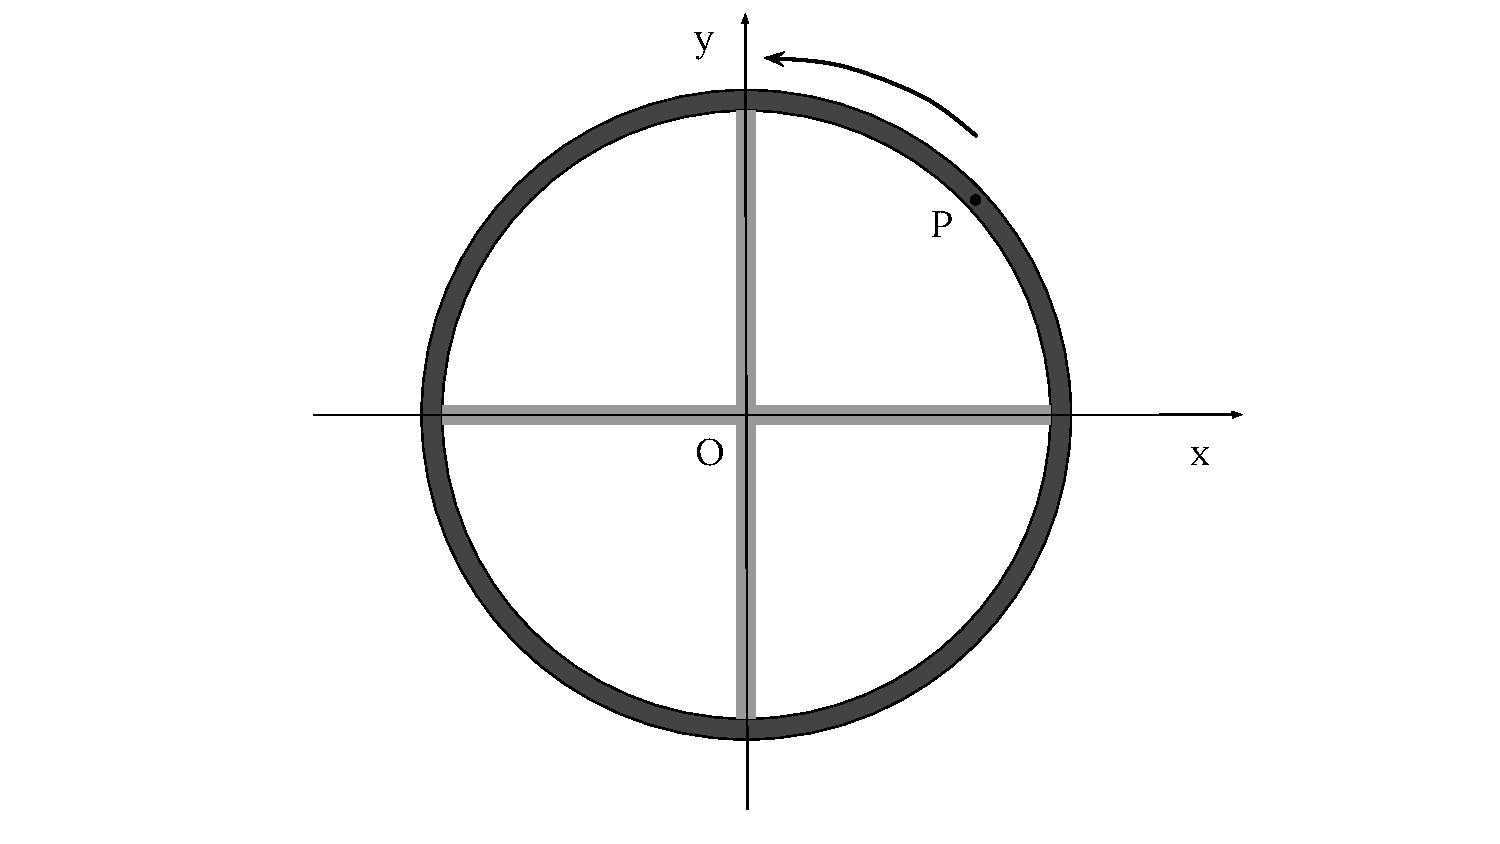
\includegraphics[scale=0.45]{ruota1.pdf}
\caption{Schema dell'esercizio: il punto $P$ si muove di moto circolare uniforme assieme alla circonferenza esterna di raggio $R$. \label{fig:ruota1} }
\end{figure}

\subsubsection*{Soluzione}
La frequenza di un moto periodico (come quello circolare uniforme) è per definizione $f=T^{-1}$. Nel nostro caso si ha:
%
\begin{gather*}
f=\frac{1}{T} \simeq \frac{1}{61} \text{s}^{-1} \simeq 0.016\; \;  \text{Hz}
\end{gather*} 
%
Chiamiamo $\vec{r}_P(t)$ la posizione del punto $P$ in un generico istante di tempo $t$ nel sistema di riferimento specificato nel testo e chiamiamo $\phi(t)$ l'angolo che $\vec{r}_P(t)$ forma con l'asse $x$, ovvero con il versore $\hat{x}$.  Dato che il moto è circolare uniforme, considerando 
una piccola variazione $\Delta t$ del tempo, avremo: 
%
\begin{gather*}
\Delta \phi = \frac{v \Delta t}{R}
\end{gather*} 
%
Di conseguenza, se $\phi(0)=0$ come detto nel testo:
%
\begin{gather*}
\phi(t) = \frac{v t}{R}
\end{gather*} 
%
Il periodo $T$ è legato alla velocità $v$ da:
%
\begin{gather*}
Tv=2\pi R \quad \Rightarrow \quad v=\frac{2 \pi R}{T}=2 \pi R f
\end{gather*} 
%
(perché in un tempo $T$ il punto $P$ si muove di una lunghezza pari al perimetro della circonferenza, ovvero $2\pi R$). Quindi: 
%
\begin{gather*}
\phi(t) = 2 \pi f t
\end{gather*} 
%
Se scriviamo $\vec{r_P}(t)$ in coordinate cartesiane 
$(x_P(t), y_P(t))$ avremo:
%
\begin{equation*}
 \left\{\begin{array}{lr}
  x_P(t)= R \cos(\phi(t))=R \cos(2 \pi f t) \\
  y_P(t)= R \sin(\phi(t))=R \sin(2 \pi f t)\\
        \end{array}\right.
\end{equation*}
%
(abbiamo usato basilari relazioni trigonometriche). Come voluto si ha:
%
\begin{equation*}
 \left\{\begin{array}{lr}
  x_P(t=0)=R \cos(0)= R \\
  y_P(t=0)= R \sin(0)=0\\
        \end{array}\right.
\end{equation*}
%
In coordinate polari il moto è invece descritto semplicemente da: 
%
\begin{gather*}
r(t)=R \\
\phi(t) = 2 \pi f t
\end{gather*}
%
La velocità in coordinate cartesiane si trova derivando rispetto a $t$ la legge oraria scritta sopra. Ricordando la regola della derivata di una funzione composta, si ha per esempio:
%
\begin{gather*}
(v_P)_x(t)= R \frac{d \cos \big(\phi(t)\big)}{dt} = R \frac{d \cos (\phi)}{d\phi} \frac{d \phi}{dt}= -R \sin \big(\phi(t) \big) \frac{d \phi}{dt}  = \\
= -2 \pi f R \sin \big(\phi(t)\big) = - v \sin \big(2 \pi f t \big)
\end{gather*} 
%
Procedendo similmente con l'altra componente si trova:
% 
\begin{equation*}
 \left\{\begin{array}{lr}
  (v_P)_x(t=0)= - v \sin(2 \pi f t) \\
  (v_P)_y(t=0)= + v \cos(2 \pi f t) \\
        \end{array}\right.
\end{equation*}
%
In effetti questo risultato si poteva ottenere in modo più 
facile graficamente (si veda la Figura \ref{fig:ruota vec}). Come \text{check} possiamo notare che:
%
\begin{equation*}
 \left\{\begin{array}{lr}
  (v_P)_x(t=0)= 0\\
  (v_P)_y(t=0)= + v\\
        \end{array}\right.
\end{equation*}
% 
cioè la velocità al tempo $t=0$ è diretta lungo l'asse delle $y$, con verso positivo. Questo torna se pensiamo che $P$ all'inizio si trova sull'asse delle $x$ e quindi la sua velocità, che è sempre \textit{tangente} alla circonferenza, dev'essere diretta lungo $y$ e puntare verso l'alto (poiché il moto avviene in verso antiorario). 

 \begin{figure}[!ht]
 \centering
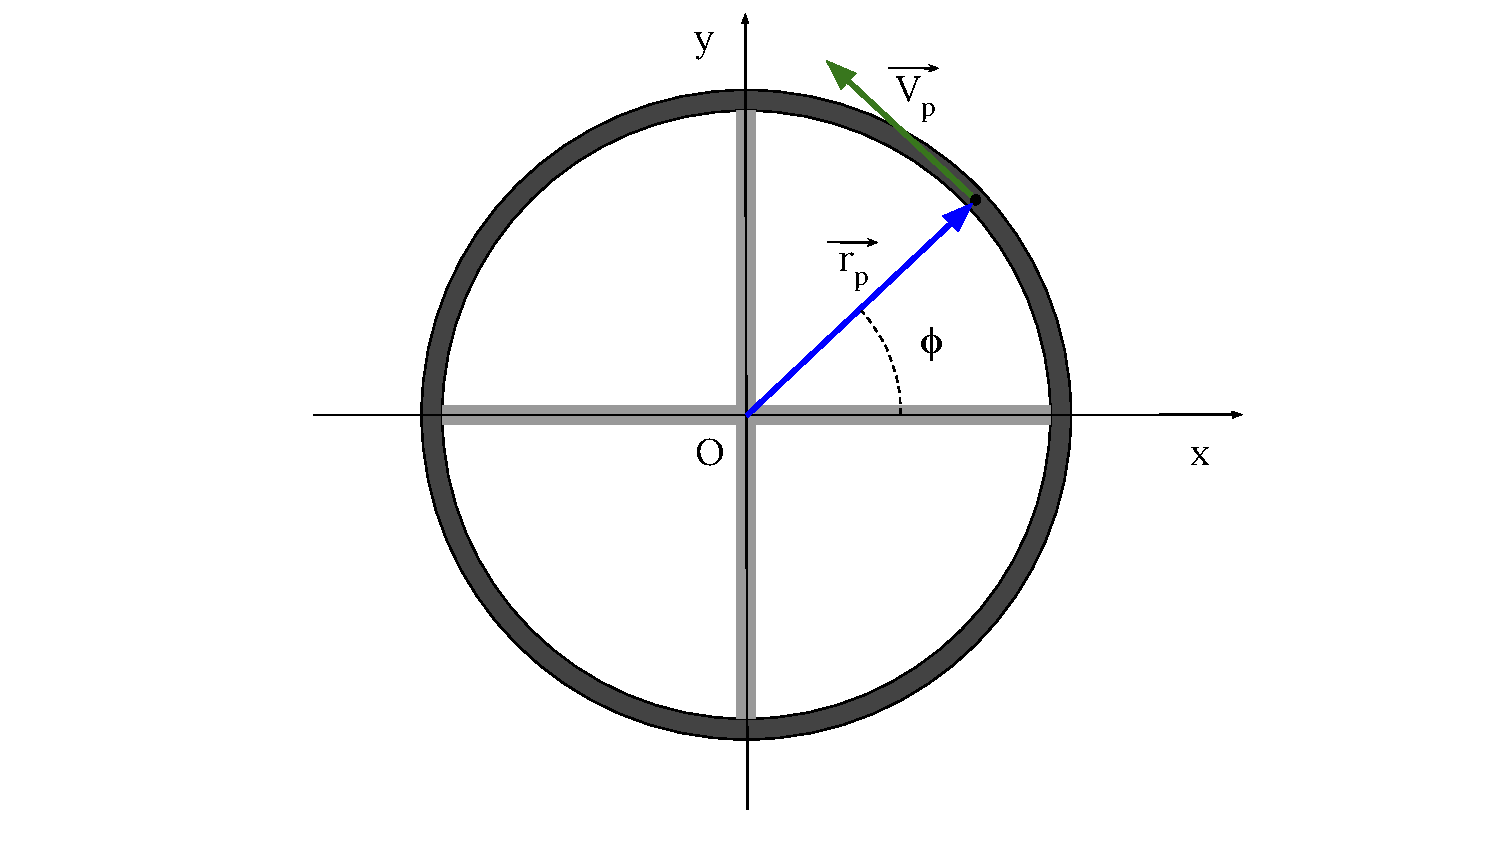
\includegraphics[scale=0.45]{ruota2.pdf}
\caption{Vettore $\vec{r_P}(t)$ (posizione di $P$) e vettore $\vec{v_P}(t)$ (velocità di $P$) ad un generico istante di tempo $t$. \label{fig:ruota vec} }
\end{figure}

In coordinate polari il vettore velocità sarà: 
%
\begin{equation*}
\vec{v_P}= v\hat{\phi}
\end{equation*}
%

Il vettore accelerazione in coordinate cartesiane si può ottenere derivando rispetto a $t$ le due componenti del vettore $\vec{v_P}(t)$ ricavate sopra. Alternativamente
ci si può ricordare che un punto materiale che si muove di moto circolare uniforme ha un vettore accelerazione $\vec{a}_P(t)$ diretto \textit{radialmente}, cioè parallelo a $\vec{r_P}(t)$ e ad $\hat{r}$, ma con verso opposto.  Inoltre il modulo di $\vec{a}_P(t)$ è costante e pari a $a=\frac{v^2}{R}$.  
Quindi: 
%
\begin{equation*}
 \left\{\begin{array}{lr}
  (a_P)_x(t)=-\frac{v^2}{R}  \cos(2 \pi f t)\\
  (a_P)_y(t)= - \frac{v^2}{R}  \sin(2 \pi f t)\\
        \end{array}\right.
\end{equation*}
%
In coordinate polari:
\begin{gather*}
\vec{a}_P(t)=-a\hat{r}
\end{gather*}
%
Se vogliamo esprimere $a$ in funzione di $f$ basta sostituire $v=2 \pi R f$: 
%
\begin{gather*}
a=\frac{v^2}{R}= 4 \pi^2 R f^2
\end{gather*}
%
Se si vuole $a=g$ allora:
%
\begin{gather*}
4 \pi^2 R f^2=g 
\end{gather*}
%
da cui ricaviamo: 
%
\begin{gather*}
R=\frac{g}{4 \pi^2 f^2} 
\end{gather*}
%
Sostituendo il valore numerico di $f$ troviamo: 
%
\begin{gather*}
R \approx 920 \; \; \text{m} 
\end{gather*}
%
Questa è la dimensione della stazione spaziale che si vede nel film! Se si vuole aumentare di un fattore di $2$ la dimensione della stazione, cioè $R \; \rightarrow \;2R$, mantenendo $a=g$ allora bisogna diminuire $f \; \rightarrow \; f/\sqrt{2}$; infatti $f^2 R$ deve rimanere invariato (è uguale a $\frac{g}{4 \pi^2}$). Allora: $v=2 \pi R f \; \rightarrow \;  2 \pi 2R \frac{f}{\sqrt{2}}=\sqrt{2}v$, cioè la frequenza deve diminuire ma la velocità esterna aumentare.

\subsection{Moto di un parapendio \rstar\rstar\rstar} 
Un parapendio effettua la sua discesa seguendo una traiettoria \textit{elicoidale} che in un sistema di coordinate cartesiane è descritto da:
%
\[
\begin{cases}
	x=A\cos\omega t \\
    y=A\sin\omega t \\
    z=-\eta t
\end{cases}
\]
%
Con $A=5\;\text{m}$, $\omega=0.628\;\text{rad/s}$ e $\eta=1.2\;\text{m/s}$. Ricordiamo che $\omega$ è legata alla frequnza $f$ del moto dalla relazione: $\omega=2 \pi f$. Rispondere alle seguenti richieste:

\begin{enumerate}[label=\alph*)]
\item  Scrivere il vettore posizione che identifica il moto del parapendio nello spazio sia in coordinate cartesiane sia cilindriche.
\item Scrivere l'equazione della traiettoria in coordinate cilindriche ($r\phi z$).
\item Limitando il moto al piano $xy$ scrivere il raggio di rotazione, trarne le conclusioni sul tipo di moto.
\item Mostrare che il modulo della velocità limitata al piano $xy$ è costante nel tempo e trarre conclusioni aggiuntive sul tipo di moto. Calcolare il valore in km/h.
\item Calcolare il periodo di rotazione.
\item Calcolare il modulo del vettore velocità complessivo in km/h
\end{enumerate}

\subsubsection*{Soluzione}

\begin{enumerate}[label=\alph*)]
\item  Il parapendio può essere identificato nello spazio grazie al raggio vettore: 
%
\begin{equation*}
\vec{r}(t)=r_x(t)\hat{x}+r_y(t)\hat{y}+r_z(t)\hat{z}=r(t)\hat{r}(t)+r_z(t)\hat{z}
\end{equation*}
%
Notiamo come non sia presente una componente tangente nella versione polare, fatto naturale quando si parla di traiettoria di un punto in quanto la posizione è descritta univocamente nel piano già dalla distanza dall'origine e dalla direzione del vettore radiale (chi se ne volesse convincere può calcolare le componenti polare del vettore descritto nel testo dell'esercizio usando le relazioni trovate nell'esercizio \ref{subsec:polar}). Notiamo inoltre come i versori cartesiani non dipendano dal tempo, mentre quelli polari sì.
\item Usando le relazioni fra quantità cartesiane e polari si ottiene una traiettoria:
%
\[
\begin{cases}
	r=\sqrt{r_x^2+r_y^2}=A \\
    z=-\eta t
\end{cases}
\]
%
\item Per ricavare il raggio della rotazione basta limitarci al piano $xy$, usando il teorema di Pitagora si ottiene facilmente:
%
\begin{equation*}
r=\sqrt{A^2\cos^2\omega t+A^2\sin^2\omega t}= A 
\end{equation*}
%
(Si è usato il fatto che per ogni angolo $\alpha$, $\cos^2(\alpha) + \sin^2(\alpha)=1$). Da questo risultato si deduce che siamo in presenza di un moto circolare (il raggio A non dipende infatti dal tempo) e la velocità radiale deve essere uguale a zero (ma \textit{non} l'accelerazione radiale).
\item Calcoliamo la velocità limitata al piano xy, considerando solo le componenti x e y del raggio vettore e deriviamole:
%
\begin{gather*}
\vec{v}=\dv{t}\vec{r}(t)=\dv{t}[r_x(t)]\hat{x}+\dv{t}[r_y(t)]\hat{y}\\
\vec{v}=-A\omega\sin(\omega t)\hat{x}+A\omega\cos(\omega t)\hat{y}
\end{gather*}
%
Il modulo di tale vettore è:
%
\begin{gather*}
\qty|\vec{v}|=\sqrt{(-A\omega)^2\sin^2(\omega t)+(A\omega)^2\cos^2(\omega t)}=\sqrt{A^2\omega^2}\approx 3.36\;\frac{\text{m}}{\text{s}}=12.10\;\frac{\text{km}}{\text{h}} 11.304\;\frac{\text{km}}{\text{h}}
\end{gather*}
%
Quindi effettivamente il modulo di questa velocità non dipende dal tempo. Avevamo prima osservato che la velocità radiale dovesse essere uguale a zero, unendo il fatto che il modulo rimane costante nel tempo allora anche l'altra componente, la velocità tangenziale, deve rimanere costante nel tempo quindi l'accelerazione tangenziale deve essere uguale a zero. E' quindi un moto circolare uniforme.
\item Il periodo di rotazione del parapendio si ricava facilmente dalla formula:
%
\begin{equation*}
T=\frac{1}{f}=\frac{2\pi}{\omega}\approx 10\;\text{s}
\end{equation*}
%
\item Calcoliamo adesso il modulo della velocità complessiva derivando il raggio vettore:
%
\begin{gather*}
\vec{V}=\dv{t}\vec{r}(t)=\dv{t}[r_x(t)]\hat{x}+\dv{t}[r_y(t)]\hat{y}+\dv{t}[r_z(t)]\hat{z} \\
\vec{V}=-A\omega\sin(\omega t)\hat{x}+A\omega\cos(\omega t)\hat{y}-\eta\hat{z}\\
\qty|\vec{V}|=\sqrt{(-A\omega)^2\sin^2(\omega t)+(A\omega)^2\cos^2(\omega t)+\eta^2}=\sqrt{A^2\omega^2+\eta^2}\approx 3.36\;\frac{\text{m}}{\text{s}}=12.10\;\frac{\text{km}}{\text{h}}
\end{gather*}
%
Notiamo che anche il modulo della velocità complessiva è costante.
\end{enumerate}

\chapter{Dinamica del punto materiale}

\graphicspath{{./figure/4/}}


\section{Esercizi}

\subsection*{Esercizio 1}
Determinare la forza necessaria per imprimere un'accelerazione di $2\;\text{m/s}^2$ a una scatola di massa $m=25\;\text{kg}$ appoggiata su una superficie di ghiaccio (assumiamo nessun attrito).

\subsubsection*{Soluzione}
Dobbiamo usare la II legge di Newton, in questo caso essendo una la forza in gioco non ci sarà bisogno di utilizzare la sommatoria:
%
\begin{gather*}
\vec{\text{F}}=m\vec{a}
\end{gather*}
%
Visto che nel testo non si fa riferimento a una direzione particolare del moto possiamo porre il riferimento in modo da ridurre il problema ad un moto unidimensionale, a questo punto possiamo far cadere la notazione vettoriale. Riepiloghiamo la situazione in Figura \ref{fig:4-e-1}. Con i dati del problema otteniamo:
%
\begin{gather*}
F=ma \qquad F=25\;\text{kg} \cdot 2\;\text{m/s}^2 = 50\; \text{N}
\end{gather*}
%

\begin{figure}[!ht]
\centering
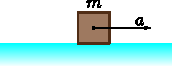
\includegraphics[scale=2]{e-1.pdf}
\caption{Cassa che accelera su superficie ghiacciata.} 
\label{fig:4-e-1} 
\end{figure}

\subsection*{Esercizio 2}
Tramite una corda si vuole far accelerare orizzontalmente una massa di $950\;\text{kg}$. La tensione applicata è $F_T=500\;\text{N}$. Quale accelerazione avrà il corpo? Supporre l'assenza di attriti.

\subsubsection*{Soluzione}
Visto sulla massa agisce una forza, per il II principio, quest'ultima avrà una certa accelerazione. Avremo quindi:
%
\begin{gather*}
a=\frac{F_T}{m} \qquad a=\frac{500\;\text{N}}{950\;\text{kg}}\approx 0.526 \;\frac{\text{kg}\;\text{m}}{\text{kg}\;\text{s}^2}= 0.526 \;\frac{\text{m}}{\text{s}^2}
\end{gather*}
%

\subsection*{Esercizio 3}
Una fune viene utilizzata per accelerare \textit{verticalmente} una massa a $+1\;\text{m/s}^2$. La tensione applicata è di $F_T=70\;\text{N}$. Calcolare il valore della massa del corpo. 

\subsubsection*{Soluzione}
Visto che stiamo accelerando \textit{verticalmente} una massa dovremo tener conto anche della forza peso $F_G$ (non più bilanciata dalla forza normale perché non appoggiata a una superficie), il diagramma di corpo libero è riportato in Figura \ref{fig:4-e-3}.

\begin{figure}[!ht]
\centering
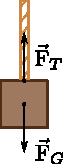
\includegraphics[scale=2]{e-3.pdf}
\caption{Massa accelerata verticalmente, si noti la forza peso e la tensione.} 
\label{fig:4-e-3} 
\end{figure}

Utilizziamo dunque la II legge di Newton. Abbiamo un primo esempio di come sia importante ricordare la natura vettoriale di tale legge: infatti le due forze sono rivolte in versi opposti. Per praticità orientiamo l'asse $y$ verso l'alto ottenendo:
%
\begin{gather*}
(F_T-F_G)\hat{y}=ma_y\hat{y} \quad \Longrightarrow \quad F_T= m(a_y+g) \\
m=\frac{F_T}{a_y+g}=\frac{70\;\text{N}}{(1+9.8)\;\text{m/s}^2}\approx 6.5\;\text{kg}
\end{gather*}
%

\subsection*{Esercizio 4}
Un uomo sale su una bilancia in un ascensore fermo. Quando l'ascensore comincia a muoversi la bilancia segna, per un breve tempo, il 75\% del peso normale della persona. Calcolare l'accelerazione dell'ascensore (modulo e verso). 

\subsubsection*{Soluzione}
Analizziamo prima la situazione di ascensore fermo: l'accelerazione sarà $\vec{a}=0$, dunque siamo in una condizione di \textit{statica} e la II legge di Newton si scrive ($\vec{\text{F}}_N$ forza normale esercitata dalla bilancia sull'uomo):
%
\begin{gather*}
\vec{\text{F}}_G+\vec{\text{F}}_N=0 \quad \Longrightarrow \quad \vec{\text{F}}_N=-m\vec{g}
\end{gather*}
%
Dunque è facile concludere che la forza normale è uguale in modulo a quella di gravità ma ha verso opposto.

Passiamo alla situazione con l'ascensore in movimento: stavolta l'accelerazione non sarà uguale a 0! La forza peso è uguale in tutte le situazioni ($\vec{\text{F}}_G=m\vec{g}$), quello che cambia sarà quindi la forza normale (e infatti l'indicazione che vediamo sulla bilancia è proprio dovuta alla forza normale che i componenti interni esercitano sull'uomo). La II legge di Newton si scriverà allora:
%
\begin{gather*}
\vec{\text{F}}_G+\vec{\text{F}}_N'=m\vec{a}
\end{gather*}
%
Dal testo sappiamo che il peso misurato dalla bilancia nella situazione dinamica è il 75\% di quello rispetto all'ascensore fermo ovvero $\vec{\text{F}}_N'=0.75\,\vec{\text{F}}_N$. Adesso è facile ricavare l'accelerazione dell'ascensore:
%
\begin{gather*}
m\vec{g}+0.75\vec{\text{F}}_N=m\vec{a} \quad \Longrightarrow \quad m\vec{g}-0.75m\vec{g}=m\vec{a} \\
0.25\vec{g}=\vec{a}
\end{gather*}
%
Ovvero l'accelerazione dell'ascensore ha lo stesso verso di quella di gravità (rivolta verso il basso) e modulo pari a un quarto di $g$. In Figura \ref{fig:4-e-4} il diagramma di corpo libero del problema.

\begin{figure}[!ht]
\centering
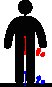
\includegraphics[scale=3]{e-4.pdf}
\caption{Diagramma corpo libero: sull'uomo agisce la forza peso e la reazione normale.} 
\label{fig:4-e-4} 
\end{figure}

\subsection*{Esercizio 5}
Una particella si muove con velocità costante $\vec{v}= (3\;\text{m/s})\hat{x} - (5\;\text{m/s})\hat{y}$ con due forze che agiscono su di essa. Sapendo che $\vec{\text{F}}_1=(4\;\text{N})\hat{x} + (7\;\text{N})\hat{y}$, determinare $\vec{\text{F}}_2$.

\subsubsection*{Soluzione}
Sappiamo che la velocità è costante ($v=k$) quindi l'accelerazione della particella sarà pari a zero, infatti:
%
\begin{gather*}
a=\dv{v}{t}=\dv{t}[k]=0
\end{gather*}
%
In virtù di questo possiamo scrivere la II equazione di Newton come:
%
\begin{gather*}
\vec{\text{F}}_1+\vec{\text{F}}_2=0 \quad \Longrightarrow \quad \vec{\text{F}}_2=-\vec{\text{F}}_2
\end{gather*}
%
Ovvero la forza $\vec{\text{F}}_2$ deve essere uguale in modulo a $\vec{\text{F}}_1$ ma opposta in verso così da rendere 0 la risultante delle forze agenti sul sistema.

\subsection*{Esercizio 6}
Un oggetto di massa $m=5.00\;\text{kg}$ è soggetto a 3 forze che gli imprimono un'accelerazione $a=(-5.00\;\text{m/s}^2)\hat{x}+(3.00\;\text{m/s}^2)\hat{y}$. Sapendo che $\vec{\text{F}}_1=(13.0\;\text{N})\hat{x}+(30.0\;\text{N})\hat{y}$ e $\vec{\text{F}}_2=(8.0\;\text{N})\hat{x}+(-11.0\;\text{N})\hat{y}$, calcolare $\vec{\text{F}}_3$.

\subsubsection*{Soluzione}
Scriviamo la II legge di Newton per il problema:
%
\begin{gather*}
\vec{\text{F}}_1+\vec{\text{F}}_2+\vec{\text{F}}_3=m\vec{a} \quad \Longrightarrow \quad \vec{\text{F}}_3= m\vec{a} - \vec{\text{F}}_1 - \vec{\text{F}}_2
\end{gather*}
%
Utilizziamo i valori forniti nel testo e facciamo una somma per componenti:
%
\begin{gather*}
\vec{\text{F}}_3= [5.00\;\text{kg} \; (-5.00\;\text{m/s}^2)\hat{x}+(3.00\;\text{m/s}^2)\hat{y}] - [(13.0\;\text{N})\hat{x}+(30.0\;\text{N})\hat{y}] - [(8.0\;\text{N})\hat{x}+(-11.0\;\text{N})\hat{y}] \\
\vec{\text{F}}_3= (-46.00\;\text{N})\hat{x}+(-4.00\;\text{N})\hat{y}
\end{gather*}
%



\subsection*{Esercizio 7}
Una massa $m=5.0\;\text{kg}$ giace su un piano inclinato di angolo $\theta=30\degree$ ed è tenuta ferma da una fune collegata al muro come in Figura \ref{fig:4-e-8-1}. Calcolare la tensione della fune e la forza di reazione normale. Supponendo di tagliare la fune trovare il modulo dell'accelerazione della massa.

\begin{figure}[!ht]
\centering
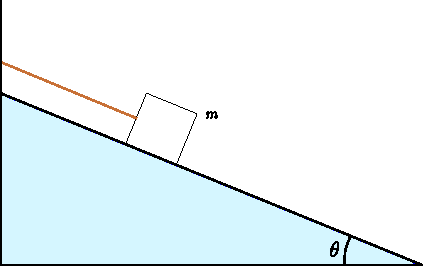
\includegraphics[scale=1]{e-8-1.pdf}
\caption{Massa collegata a una fune su piano inclinato.} 
\label{fig:4-e-8-1} 
\end{figure}

\subsubsection*{Soluzione}
Come prima cosa impostiamo un sistema di riferimento in cui un versore è parallelo al lato del piano inclinato ($\hat{e}_\parallel$) e l'altro gli è ortogonale ($\hat{e}_\perp$), così abbiamo che il prodotto scalare fra i due è 0 $\hat{e}_\parallel\cdot\hat{e}_\perp=0$, è un sistema di riferimento cartesiano ruotato come nel Problema \ref{subsec:incline}. Il diagramma di corpo libero della massa è riportato in Figura \ref{fig:4-e-8-2}.

\begin{figure}[!ht]
\centering
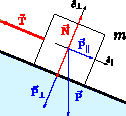
\includegraphics[scale=3]{e-8-2.pdf}
\caption{Diagramma di corpo libero con le componenti di $\vec{P}$.} 
\label{fig:4-e-8-2} 
\end{figure}

È facile mostrare (Problema \ref{subsec:incline}) che $P_\parallel=P\sin\theta$ e $P_\perp=P\cos\theta$, scriviamo quindi la II legge di Newton per la massa ($\vec{\text{N}}$ è la reazione normale del piano):
%
\begin{gather*}
\vec{\text{P}}+\vec{\text{T}}+\vec{\text{N}}=0
\end{gather*}
%
Scriviamo adesso l'equazione vettoriale per componenti, scomponendo lungo i versori parallelo e perpendicolare:
%
\begin{gather*}
(P_\parallel-T)\hat{e}_\parallel + (-P_\perp+N)\hat{e}_\perp=0
\end{gather*}
%
La condizione che si deduce è che entrambe le componenti debbano essere uguali a 0 (infatti se il corpo è in quiete il vettore accelerazione è 0 e quindi anche tutte le sue componenti). Abbiamo allora:
%
\begin{gather*}
T=P_\parallel=mg\sin\theta \quad \Longrightarrow \quad T=5.0\;\text{kg}\cdot 9.8\;\frac{\text{m}}{\text{s}^2}\cdot \frac{1}{2} = 24.5\;\text{N} \\
N=P_\perp=mg\cos\theta \quad \Longrightarrow \quad N=5.0\;\text{kg}\cdot 9.8\;\frac{\text{m}}{\text{s}^2}\cdot \frac{\sqrt{3}}{2} \approx 42.4\;\text{N}
\end{gather*}
%
Quando la fune viene recisa la massa accelererà parallelamente al piano inclinato, le componenti perpendicolari delle forze continueranno ad annullarsi, mentre per quelle parallele non avremo più la tensione:
%
\begin{gather*}
P_\parallel=ma_\parallel \quad \Longrightarrow \quad a_\parallel=\frac{P_\parallel}{m}=\frac{24.5\;\text{N}}{5.0\;\text{kg}}=4.9\;\frac{\text{m}}{\text{s}^2}
\end{gather*}
%

\subsection*{Esercizio 8}
Una scatola di massa $m_1=15\;\text{kg}$ è ferma su un tavolo. Una fune legata alla scatola sale fino a una carrucola e all'altro lato è appeso un contrappeso di massa $m_2=3\;\text{kg}$, la situazione è descritta in Figura \ref{fig:4-e-9-1}. Determinare la forza di reazione normale del tavolo sulla scatola. Quanto varrebbe nel caso in cui $m_2 \geq m_1$?

\begin{figure}[!ht]
\centering
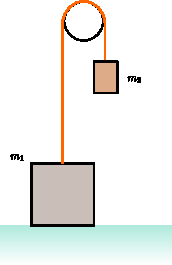
\includegraphics[scale=1.5]{e-9-1.pdf}
\caption{Scatola legata ad un contrappeso tramite una carrucola.} 
\label{fig:4-e-9-1} 
\end{figure}

\subsubsection*{Soluzione}
Iniziamo tracciando il diagramma di corpo libero delle due masse, è riportato in Figura \ref{fig:4-e-9-2}.

\begin{figure}[!ht]
\centering
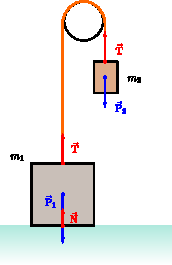
\includegraphics[scale=2]{e-9-2.pdf}
\caption{Scatola legata ad un contrappeso tramite una carrucola.} 
\label{fig:4-e-9-2} 
\end{figure}

Conviene iniziare l'analisi dal corpo soggetto ad un minor numero di forze, quindi da $m_2$. Scriviamo la II legge di Newton:
%
\begin{gather*}
\vec{\text{P}}_2+\vec{\text{T}}=0 \quad \Longrightarrow \quad \vec{\text{T}}=-\vec{\text{P}}_2=-m_2\vec{g}
\end{gather*}
%
Teniamo da parte questa relazione (che ci ha fatto trovare un'incognita del nostro problema). Passiamo all'analisi della massa $m_1$:
%
\begin{gather*}
\vec{\text{P}}_1+\vec{\text{T}}+\vec{\text{N}}=0 \\
(-P_1+N+T)\hat{y}=0 \quad \Longrightarrow \quad P_1=N+T
\end{gather*}
%
Sostituendo l'espressione per la tensione precedentemente individuata ed esplicitando i valori della forza peso si ottiene:
%
\begin{gather*}
m_1g=N+m_2g \quad \Longrightarrow \quad N=(m_1-m_2)g \quad \rightarrow \quad N=(15-3)\;\text{kg} \cdot 9.8 \;\frac{\text{m}}{\text{s}^2} \approx 118\;\text{N}
\end{gather*}
%
Nel caso in cui $m_1=m_2$ si ottiene che la reazione normale del tavolo è pari a 0. Questo può essere visto come caso limite. Se tenessimo il modello sopra descritto e provassimo a vedere $m_2>m_1$ otterremmo una reazione normale del tavolo negativa, questo è indice di un errore perché un tavolo non può chiaramente attrarre un oggetto a sé. L'errore in questo caso sarebbe aver utilizzato la seconda legge di Newton con accelerazione pari a 0 (caso statico) quando in questa ipotesi si ottiene, anche intuitivamente, che la massa $m_1$ viene sollevata verso l'alto con una certa accelerazione (sarà l'oggetto di un problema successivo). In altre parole: in questo caso non esistono soluzioni statiche del problema. \\ 

Questo esercizio vuole rimarcare 2 fatti: il primo è che la reazione normale \textit{non} è (sempre) l'opposto della forza peso; il secondo è che non sempre si può applicare un modello fisico fatto su certe condizioni ad altre senza modificarlo opportunamente.

\subsection*{Esercizio 9}
Una massa $m=4\;\text{kg}$ è fissata al centro di una fune. L'angolo che formano i tratti di fune con l'orizzontale è $\theta=15\degree$. Trovare la tensione della fune. La situazione è riportata in Figura \ref{fig:4-e-10-1}.

\begin{figure}[!ht]
\centering
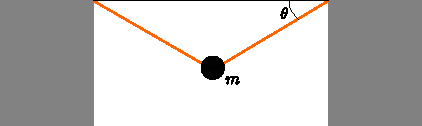
\includegraphics[scale=1.5]{e-10-1.pdf}
\caption{Massa sostenuta da due funi.} 
\label{fig:4-e-10-1} 
\end{figure}

\subsubsection*{Soluzione}
Riferiamoci al diagramma di corpo libero di Figura \ref{fig:4-e-10-2}. Le tensioni delle funi sono uguali per un semplice fatto di simmetria (il corpo è al centro della fune).

\begin{figure}[!ht]
\centering
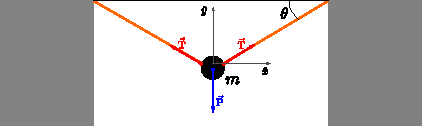
\includegraphics[scale=1.5]{e-10-2.pdf}
\caption{Diagramma di corpo libero della massa.} 
\label{fig:4-e-10-2} 
\end{figure}

La II legge di Newton si scrive quindi:
%
\begin{gather*}
\vec{\text{P}}+2\vec{\text{T}}=0
\end{gather*}
%
Visto che il corpo è fermo la componente verticale dell'accelerazione sarà 0, scriviamo quindi l'equazione precedente lungo quella componente:
%
\begin{gather*}
(\vec{\text{P}}+2\vec{\text{T}})\cdot\hat{y}=0 \quad \Longrightarrow \quad -P +2T\sin\theta=0
\end{gather*}
%
Possiamo quindi ricavare agevolmente il valore della tensione:
%
\begin{gather*}
T=\frac{P}{2\sin\theta}=\frac{mg}{2\sin\theta} \quad \Longrightarrow \quad T \approx \frac{4\;\text{kg}\cdot 9.8 \;\frac{\text{m}}{\text{s}^2}}{2\cdot0.26}\approx 75.4 \;\text{N}
\end{gather*}
%

\subsection*{Esercizio 10}
Una cassa di massa $m=26\;\text{kg}$ scivola su un pavimento con coefficiente di attrito dinamico $\mu_d=0.30$. Quale forza orizzontale è necessaria per far muovere la cassa a velocità costante? Se non ci fosse attrito?

\subsubsection*{Soluzione}
Tracciamo il diagramma di corpo libero per la cassa, è in Figura \ref{fig:4-e-11}. Ricordiamo che la forza di attrito dinamico ha direzione parallela alla superficie di contatto, verso opposto alla velocità dell'oggetto e modulo $F_a=\mu_d N$.

\begin{figure}[!ht]
\centering
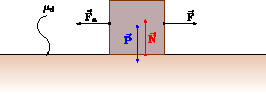
\includegraphics[scale=2]{e-11.pdf}
\caption{Diagramma di corpo libero, notare la forza di attrito} 
\label{fig:4-e-11} 
\end{figure}

Scriviamo la II legge di Newton:
%
\begin{gather*}
\vec{\text{F}}+\vec{\text{F}_a}+\vec{\text{N}}+\vec{\text{P}}=m\vec{a}
\end{gather*}
%
Visto che la cassa si muove sul piano la sua accelerazione verticale $a_y$ deve essere uguale a 0.
%
\begin{gather*}
N-P=0 \quad	\Longrightarrow \quad N=P=mg
\end{gather*}
%
Mentre per quanto riguarda la componente orizzontale abbiamo, utilizzando l'espressione prima ricavata per la reazione normale $N$:
%
\begin{gather*}
F-F_a=ma_x \quad	\Longrightarrow \quad F-\mu_d mg=ma_x
\end{gather*}
%
Se vogliamo che il corpo si muova con velocità costante, la sua accelerazione deve essere uguale a 0 quindi anche $a_x=0$. Quindi:
%
\begin{gather*}
F=\mu_d mg \quad	\Longrightarrow \quad F=0.30 \cdot 26\; \text{kg} \cdot 9.8 \;\frac{\text{m}}{\text{s}^2} \approx	76\;\text{N}
\end{gather*}
%
Se invece non ci fosse attrito ($\mu_d=0$) è ovvio che $F=0$, perché corpi che non subiscono forze esterne si muovono di moto rettilineo uniforme (cioè a velocità costante).

\subsection*{Esercizio 11}
Affinché una scatola di massa $m=7\;\text{kg}$ inizi a muoversi lungo il pavimento orizzontale di una stanza, è necessario applicare una forza di $40\;\text{N}$. Quale è il coefficiente di attrito statico fra scatola e pavimento? Se la forza continua ad essere applicata la scatola subisce un'accelerazione $a=0.40\;\text{m/s}^2$, trovare il coefficiente di attrito dinamico.

\subsubsection*{Soluzione}
Il diagramma di corpo libero è uguale a quello dell'esercizio precedente (Figura \ref{fig:4-e-11}). Anche la II equazione di Newton si scrive allo stesso modo: 
%
\begin{gather*}
\vec{\text{F}}+\vec{\text{F}_a}+\vec{\text{N}}+\vec{\text{P}}=m\vec{a}
\end{gather*}
%
L'unica differenza è che in questo caso $F_a$ è una forza di attrito \textit{statico} che non ha un valore fisso ma ha un \textit{massimo} valore assumibile ($F_a\leq\mu_sN$), dopo quel valore l'oggetto inizierà a muoversi e a subire attrito \textit{dinamico} ($F_a=\mu_dN$). Per ricavare la forza di attrito statico è necessario comprendere che anche se abbiamo un'incognita in più nel nostro problema questo viene bilanciato dall'avere il corpo \textit{fermo} come condizione ulteriore.

Dall'equilibrio verticale otteniamo anche in questo caso:
%
\begin{gather*}
N-P=0 \quad	\Longrightarrow \quad N=P=mg
\end{gather*}
%
Dall'equilibro orizzontale ($a_x=0$), necessario per avere attrito statico abbiamo:
%
\[
\begin{cases}
F-F_a=0 \quad	\Longrightarrow \quad F_a=F \qquad \\ 
F_a\leq\mu_sN
\end{cases}
\]
%
Fermiamoci a ragionare sul significato di quello che abbiamo scritto: la forza che è applicata sulla scatola $F$ è la forza \textit{minima} per farla muovere, avremo quindi, nel limite della condizione in cui la scatola è ferma, la forza \textit{massima} di attrito \textit{statico} che può essere esercitata ovvero $F_a^{max}=\mu_sN$ . Dunque ricaviamo, usando l'espressione precedentemente ricavata per N:
%
\[
\begin{cases}
F_a^{max}=F      \\ 
F_a^{max}=\mu_sN
\end{cases}
\Longrightarrow \quad F=\mu_sN \quad \Longrightarrow \quad \mu_s=\frac{F}{mg} \quad \Longrightarrow \quad \mu_s=\frac{40\;\text{N}}{7\;\text{kg}\cdot 9.8 \;\frac{\text{m}}{\text{s}^2}}\approx 0.58
\]
%
Nel caso la forza continui ad essere applicata il corpo inizierà a muoversi e risentirà dell'attrito dinamico (in modulo minore dell'attrito massimo statico), avremo quindi una certa accelerazione orizzontale ricavabile dalla II legge di Newton applicata a detta direzione:
%
\begin{gather*}
F-F'_a=ma_x \quad	\Longrightarrow \quad F-ma_x=N\mu_d
\end{gather*}
%
Da cui facilmente ricaviamo:
%
\begin{gather*}
\mu_d=\frac{F-ma_x}{mg} \quad	\Longrightarrow \quad \mu_d=\frac{40\;\text{N}-7\;\text{kg}\cdot 0.40 \;\frac{\text{m}}{\text{s}^2}}{7\;\text{kg}\cdot 9.8 \;\frac{\text{m}}{\text{s}^2}}\approx 0.54
\end{gather*}
%
Notiamo che, come ci si aspettava, $\mu_s>\mu_d$.

\subsection*{Esercizio 12}
Una persona è in piedi su un treno che sta accelerando a $0.10g$, quale è il minimo coefficiente di attrito statico fra i piedi della persona e il pavimento necessario per far sì che la persona non scivoli?

\subsubsection*{Soluzione}
Affinché la persona non scivoli è necessario che sia \textit{ferma} rispetto al sistema di riferimento del treno, ovvero che abbia la sua stessa accelerazione. La forza in grado di fornire questa accelerazione è la forza di attrito statico fra il pavimento e i piedi della persona. In Figura \ref{fig:4-e-13} riportiamo il diagramma di corpo libero.

La II legge di Newton si scrive:
%
\begin{gather*}
\vec{\text{F}_a}+\vec{\text{N}}+\vec{\text{P}}=m\vec{a}
\end{gather*}
%
Dunque imponiamo l'equilibrio verticale ($a_y=0$):
%
\begin{gather*}
N-P=0 \quad	\Longrightarrow \quad N=P=mg
\end{gather*}
%
Mentre per la componente orizzontale abbiamo, trattandosi di attrito statico:
%
\[
\begin{cases}
F_a=ma_x \quad\\ 
F_a\leq\mu_sN
\end{cases}
\Longrightarrow \quad  ma_x\leq\mu_sN \quad \Longrightarrow ma_x\leq\mu_smg
\]
%
Visto che nel testo del problema si chiede il valore \textit{minimo} dovremo risolvere:
%
\begin{gather*}
a_x=\mu_sg \quad \Longrightarrow \quad \mu_s=\frac{a_x}{g}=\frac{0.10g}{g}=0.10
\end{gather*}
%

\begin{figure}[!ht]
\centering
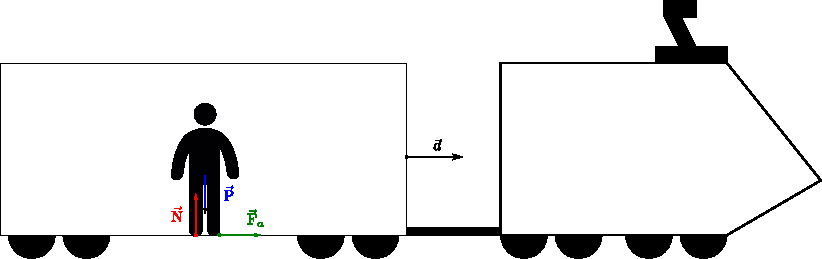
\includegraphics[scale=1.2]{e-13.pdf}
\caption{Diagramma di corpo libero della persona sul treno} 
\label{fig:4-e-13} 
\end{figure}





\pagebreak

\subsection*{Esercizio 13}
Due scatole sono appoggiate, una sopra l'altra, su un tavolo. La scatola a inferiore ha una massa $m_1=20\;\text{kg}$ mentre quella superiore ha massa $m_2=10\;\text{kg}$. Determinare le forze di reazioni normali che il tavolo esercita su $m_1$ e quella che $m_1$ esercita su $m_2$.

\subsubsection*{Soluzione}
Questo esercizio è molto interessante perché richiede l'applicazione consapevole della III legge di Newton. Iniziamo riportando il diagramma di corpo libero delle masse in Figura \ref{fig:4-e-16}.

\begin{figure}[!h]
\centering
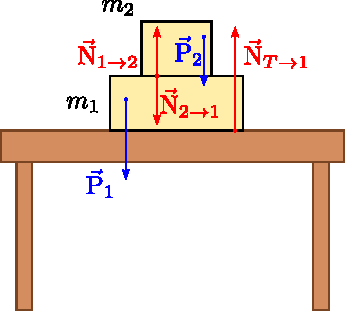
\includegraphics[scale=1.5]{e-16.pdf}
\caption{Diagramma di corpo libero, notare la coppia azione-reazione.} 
\label{fig:4-e-16} 
\end{figure}

Analizziamo prima $m_2$ scrivendo la II legge di Newton imponendo che sia ferma ($\vec{\text{N}}_{1\to2}$ è la reazione normale della scatola $m_1$ su quella $m_2$):
%
\begin{gather*}
\vec{\text{P}}_2+\vec{\text{N}}_{1\to2}=0
\end{gather*}
%
Scomponendo i vettori verticalmente abbiamo:
%
\begin{gather*}
N_{1\to2}=P_2=m_2g \quad \Longrightarrow \quad N_{1\to2}=9.8 \;\frac{\text{m}}{\text{s}^2} \cdot 10\;\text{kg}=98\;\text{N}
\end{gather*}
%
Per la III legge di Newton alla reazione normale $\vec{\text{N}}_{1\to2}$ deve corrispondere una forza accoppiata di azione, ovvero $\vec{\text{N}}_{2\to1}$ ma sappiamo che sono uguali in modulo e opposte in verso quindi $\vec{\text{N}}_{1\to2}=-\vec{\text{N}}_{2\to1}$. Applichiamo, con questa considerazione, la II legge di Newton a $m_1$:
%
\begin{gather*}
\vec{\text{P}}_1-\vec{\text{N}}_{1\to2}+\vec{\text{N}}_{T\to1}=0
\end{gather*}
%
Dunque per componenti:
%
\begin{gather*}
-P_1-N_{1\to2}+N_{T\to1}=0 \quad \Longrightarrow \quad N_{T\to1}=P_1+N_{1\to2}
\end{gather*}
%
Inserendo i valori numerici otteniamo:
%
\begin{gather*}
N_{T\to1}=9.8 \;\frac{\text{m}}{\text{s}^2} \cdot 20\;\text{kg} + 98\;\text{N}=294\;\text{N}
\end{gather*}
%

\subsection*{Esercizio 14}
Un uomo si solleva utilizzando un cesto metallico collegato con una fune a una carrucola come in Figura \ref{fig:4-e-17-1}. Con quale forza deve tirare verso il basso per sollevarsi a velocità costante? Considerare la fune priva di massa e la carrucola priva di attrito, il sistema uomo-cestello ha una massa $m=90\;\text{kg}$.


\begin{figure}[!h]
\centering
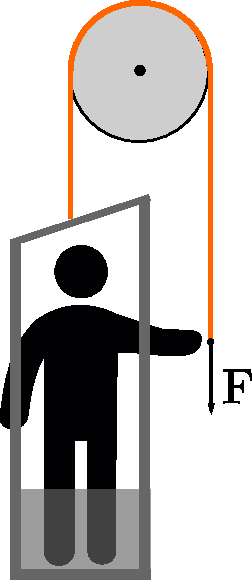
\includegraphics[scale=0.6]{e-17-1.pdf}
\caption{Situazione del problema, l'uomo esercita una forza sulla fune.} 
\label{fig:4-e-17-1} 
\end{figure}

\subsubsection*{Soluzione}
Il punto fondamentale di questo esercizio è legato alla III legge di Newton: infatti così come l'uomo esercita una forza $\vec{\text{F}}$ verso il basso sulla fune, quest'ultima eserciterà sulla mano dell'uomo una forza verso l'alto $-\vec{\text{F}}$. Dobbiamo anche notare che con le ipotesi fatte sulla carrucola e sul filo la tensione sarà unica su tutta la lunghezza della fune e sarà, in modulo, pari a $F$. Per quanto detto all'altra estremità della corda agirà una forza $\vec{\text{F}}$ e quindi sul sistema uomo-cestello agirà $-\vec{\text{F}}$.

Il diagramma di corpo libero è riportato in Figura \ref{fig:4-e-17-2}, le forze rosse sono riferite al sistema \textit{uomo-cestello} e sono applicate dalla \textit{fune} su di esso.


\begin{figure}[ht!]
\centering
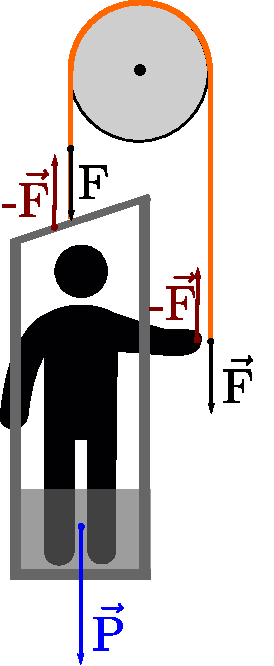
\includegraphics[scale=0.62]{e-17-2.pdf}
\caption{Diagramma di corpo libero, in rosso relativo al sistema uomo-cestello.} 
\label{fig:4-e-17-2} 
\end{figure}

Applichiamo adesso la II legge di Newton al sistema uomo-cesto, imponendo accelerazione 0 (si muove di velocità costante):
%
\begin{gather*}
\vec{\text{P}}-2\vec{\text{F}}=0 \quad \Longrightarrow \quad \vec{\text{P}}=2\vec{\text{F}}
\end{gather*}
%
Scriviamola per componenti assumendo l'asse $y$ positivo verso l'alto:
%
\begin{gather*}
F=-\frac{1}{2}mg
\end{gather*}
%
Che inserendo i dati del problema diventa:
%
\begin{gather*}
F=-\frac{1}{2} \cdot 90\;\text{kg} \cdot 9.8 \;\frac{\text{m}}{\text{s}^2}=-441\;\text{N}
\end{gather*}
%
Notare come il segno sia giustamente negativo perché la forza deve essere applicata verso il basso.


\subsection*{Esercizio 15}
Una molla di costante elastica $k$ e lunghezza a riposo $l_0=0$ è appesa verticalmente a un soffitto. 
Calcolare quanto vale il suo allungamento $\Delta l$ quando all'estremità inferiore della molla viene appesa
una massa $M$. Come cambia la risposta se la molla ha lunghezza a riposo $l_0 \neq 0$? 

\subsubsection*{Soluzione}
Mettiamoci in un sistema di riferimento cartesiano che ha come asse $\hat{y}$ la direzione dell'accelerazione di gravità ($\vec{g}=-g\hat{y}$). Tutte le forze presenti nel problema agiscono lungo $\hat{y}$, quindi il problema è unidimensionale. Possiamo quindi omettere la notazione vettoriale.\\

Le forze che agiscono sulla massa $M$ sono: la forza peso $-Mg$ e la forza elastica esercitata dalla molla: $+F_e$.
Il segno $+$ è dovuto al fatto che, a causa della geometria del sistema, la molla esercita una forza con verso positivo. 

Il valore di $F_e$ si ottiene ricordando che la forza elastica è sempre uguale al prodotto della costante elastica $k$ per l'\textit{allungamento}  della molla rispetto alla condizione di riposo. Se posizioniamo $y=0$ al livello del soffitto e chiamiamo $y_0$ la posizione di equilibrio del corpo di massa $M$ attaccato alla molla (posizione incognita), allora avremo: $F_e=k(-y_0-0)=-ky_0$. Infatti la lunghezza 
a regime della molla è $l=-y_0$  (perché la posizione di equilibrio $y_0$ sarà negativa, dato che il corpo sta sotto il soffitto), mentre la lunghezza a riposo è per ipotesi $l_0=0$, quindi l'allungamento è $l-l_0=-y_0-0=-y_0$.\\

Ora dobbiamo scrivere la somma delle forze e imporre che faccia $0$ (seconda legge di Newton). Avremo:
\begin{gather*}
-Mg-ky_0=0
\end{gather*}
da cui possiamo ricavare $y_0$:
\begin{gather*}
y_0=-\frac{Mg}{k}
\end{gather*}
L'allungamento della molla è quindi $\Delta l=-y_0=\frac{Mg}{k}$. \\

Nel caso in cui la molla abbia una lunghezza a riposo non nulla $l_0$, la forza elastica sarà $F_e=k(-y_0-l_0)=-k(y_0+l_0)$, per cui:
\begin{gather*}
-Mg-k(y_0+l_0)=0
\end{gather*}
e quindi:
\begin{gather*}
y_0=-\frac{Mg}{k}-l_0
\end{gather*}
Nel caso $l_0=0$ ovviamente riotteniamo il risultato precedente. Notiamo che sebbene la posizione di equilibrio sia cambiata rispetto a prima, 
l'allungamento $\Delta l$ della molla è il medesimo, infatti: $\Delta l=l-l_0=-y_0-l_0=\frac{Mg}{k}+l_0-l_0=\frac{Mg}{k}$ come prima.


\subsection*{Esercizio 16}
Una massa $m$ è attaccata ad un filo di lunghezza $L$. Il filo e la massa ruotano a una velocità angolare $\omega$ sul piano orizzontale $xy$ (perpendicolare
alla direzione dell'accelerazione di gravità $\vec{g}=-g\hat{z}$). Quanto vale la tensione $\tau$ esercitata dal filo? Ricordiamo
che la velocità angolare $\omega$ è legata alla frequenza $f=\frac{1}{T}$, dove $T$ è il periodo, dalla formula $\omega=2\pi f$. 
Calcolare il valore di $\tau$ per $T=0.2 \,$s,  $L=1\,$m, $m=100 \,$g. 

\subsubsection*{Soluzione}
La massa $m$ si muove di moto circolare uniforme. Di conseguenza la sua accelerazione vale in modulo $a=\frac{v^2}{L}$ ed è diretta radialmente, ovvero parallelamente alla tensione $\vec{\tau}$ esercitata dal filo. $v$ è la velocità (tangenziale) della massa $m$ e vale $v=\omega L$.\\

Dato che per la seconda legge di Newton $\vec{F}=m\vec{a}$, abbiamo:
\begin{gather*}
\tau=m \frac{(\omega L)^2}{L}=m \omega^2 L= m 4 \pi^2 f^2 L = m 4 \pi^2 T^{-2} L
\end{gather*}
Sostituendo i valori numerici indicati nel testo:
\begin{gather*}
\tau= 4 \cdot 0.1 \, \text{kg} \, \pi^2 \cdot 25 \, \text{s}^{-2} \cdot 1 \, \text{m} \simeq 98.7 N
\end{gather*}


\clearpage

\section{Problemi}
\subsection{Due forze agenti su un punto materiale \rstar}
Due forze $\vec{\text{F}}_1$ e $\vec{\text{F}}_2$ agiscono su un punto materiale di massa $m$, fra le due forze c'è un angolo $\theta$. Calcolare il vettore accelerazione dando la risposta sia per componenti sia in modulo e angolo formato con l'asse $\hat{x}$. Risolvere numericamente per $m=1.0\;\text{kg}$, $\text{F}_1=10.0\;\text{N}$, $\text{F}_2=7.0\;\text{N}$,  $\theta=90\degree$ e $\theta=30\degree$.
 
\subsubsection*{Soluzione}
Impostiamo il sistema di riferimento come in Figura \ref{fig:4-p-1} così da ridurre i calcoli per le componenti. 

 \begin{figure}[!ht]
 \centering
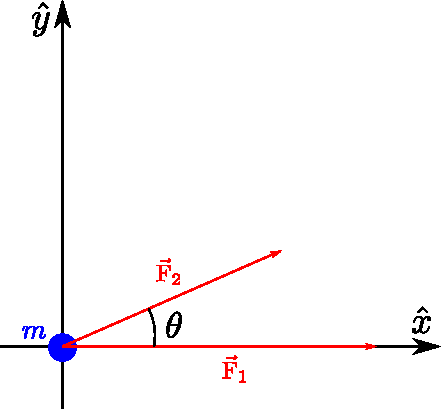
\includegraphics[scale=0.8]{p-1.pdf}
\caption{Il punto materiale è al centro e una delle due forze è allineata con un asse.} 
\label{fig:4-p-1} 
\end{figure}

Iniziamo dalla II legge di Newton che recita:
%
\begin{gather*}
\sum_i\vec{\text{F}}_i=m\vec{a}
\end{gather*}
%
Nel nostro caso avremo quindi:
%
\begin{gather*}
\vec{\text{F}}_1+\vec{\text{F}}_2=m\vec{a}
\end{gather*}
%
Procediamo a sommare le forze utilizzando le loro componenti (in ogni caso per come abbiamo scelto il riferimento $F_{1y}=0$):
%
\begin{gather*}
(F_{1x}+F_{2x})\hat{x}+F_{2y}\hat{y}=m\vec{a}
\end{gather*}
%
Otteniamo facilmente la risposta per l'accelerazione scritta per componenti:
%
\begin{gather*}
\vec{a}=\frac{1}{m}\qty[(F_{1x}+F_{2x})\hat{x}+F_{2y}\hat{y}] \\
a_x=\vec{a}\cdot\hat{x}=\frac{1}{m}(F_{1x}+F_{2x}) \qquad a_y=\vec{a}\cdot\hat{y}=\frac{F_{2y}}{m}
\end{gather*}
%
Per $\theta=90\degree$ abbiamo, con i valori di $F_1$ e $F_2$ indicati nel testo, $F_{1x}=10.0\;\text{N}$, $F_{2y}=7.0\;\text{N}$ e $F_{2x}=0\;\text{N}$, dunque:
%
\begin{gather*}
a_x=10\;\frac{\text{N}}{\text{kg}}=10\;\frac{\text{kg}\;\text{m}}{\text{kg}\;\text{s}^2}=10\;\frac{\text{m}}{\text{s}^2} \qquad a_y=7.0\;\frac{\text{N}}{\;\text{kg}}=7.0\;\frac{\text{m}}{\text{s}^2}
\end{gather*}
%
Mentre per $\theta=30\degree$ avremo la stessa componente $F_{1x}$ di prima ma:
%
\begin{gather*}
F_{2x}=F_2\cos30\degree=\frac{\sqrt{3}F_2}{2}\approx 6.1\;\text{N} \qquad  F_{2y}=F_2\sin30\degree=\frac{F_2}{2} = 3.5\;\text{N}
\end{gather*}
%
Per dare invece la risposta in modulo e angolo usiamo le relazioni ormai note dal calcolo vettoriale:
%
\begin{gather*}
a=\qty|\frac{1}{m}\qty[(F_{1x}+F_{2x})\hat{x}+F_{2y}\hat{y}]|=\frac{1}{m}\sqrt{(F_{1x}+F_{2x})^2+F_{2y}^2} \\
\tan\theta=\frac{a_y}{a_x}=\frac{F_{2y}}{F_{1y}+F_{2x}}
\end{gather*}
%
Per $\theta=90\degree$ si ha, con le componenti precedentemente calcolate:
%
\begin{gather*}
a=\frac{1}{1.0\;\text{kg}}\sqrt{10^2+7^2}\;\text{N}\approx 12\;\frac{\text{m}}{\text{s}^2} \\
\theta=\atan\qty(\frac{7.0\;\text{N}}{10.0\;\text{N}})\approx 35 \degree
\end{gather*}
%
Infine per $\theta=30\degree$:
%
\begin{gather*}
a=\frac{1}{1.0\;\text{kg}}\sqrt{(10.0+6.1)^2+3.5^2}\;\text{N}\approx 16\;\frac{\text{m}}{\text{s}^2} \\
\theta=\atan\qty(\frac{3.5\;\text{N}}{16.1\;\text{N}})\approx 12 \degree
\end{gather*}
%

\subsection{Cassonetto su strada inclinata \rstar}
Il coefficiente di attrito statico fra un cassonetto e l'asfalto è di 0.80. Trovare la massima pendenza (i.e. il massimo angolo) alla quale può essere posto il cassonetto prima di scivolare.

\subsubsection*{Soluzione}
La situazione è molto simile a quella dell'Esercizio 8 in cui si è adottato il riferimento con versori parallelo e perpendicolare al piano. Il diagramma di corpo libero della situazione è riportato in Figura \ref{fig:4-p-2}.

\begin{figure}[!ht]
\centering
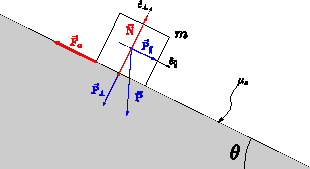
\includegraphics[scale=2]{p-2.pdf}
\caption{Diagramma di corpo libero del cassonetto sul piano inclinato.} 
\label{fig:4-p-2} 
\end{figure}

Scriviamo la II legge di Newton (ricordando che il corpo è fermo):
%
\begin{gather*}
\vec{\text{F}_a}+\vec{\text{N}}+\vec{\text{P}}=0
\end{gather*}
%
Dall'equilibrio lungo il versore perpendicolare $\hat{e}_\perp$ abbiamo:
%
\begin{gather}
N-P_\perp=0 \quad	\Longrightarrow \quad N=P_\perp=mg\cos\theta
\label{eq:4-p-2-1}
\end{gather}
%
Mentre dall'equilibrio lungo il versore parallelo $\hat{e}_\parallel$ si ha:
%
\begin{gather}
-F_a+P_\parallel=0 \quad \Longrightarrow \quad F_a=P_\parallel=mg\sin\theta
\label{eq:4-p-2-2}
\end{gather}
%
Adesso imponiamo la condizione sul massimo dell'intensità di attrito statico, superato il quale  il corpo inizia a muoversi):
%
\begin{gather*}
F_a\leq\mu_sN
\end{gather*}
%
Andiamo a sostituire le espressioni ricavate nelle eqq. \ref{eq:4-p-2-1}-\ref{eq:4-p-2-2} ottenendo la condizione richiesta:
%
\begin{gather*}
mg\sin\theta \leq \mu_s mg\cos\theta \quad \Longrightarrow \quad \tan\theta \leq \mu_s \quad \Longrightarrow \quad \theta \leq \arctan\mu_s
\end{gather*}
%
Visto che vogliamo il \textit{massimo} angolo prenderemo l'uguaglianza, con i dati del problema otteniamo:
%
\begin{gather*}
\theta^{max} = \arctan 0.80 \approx 39 \degree
\end{gather*}
%

\subsection{Massa tenuta da due molle \rstar}
Una massa $m$ è collegata (come in Figura \ref{fig:4-p-6-1}) a due molle di costante elastica $k$ e $2k$ di lunghezza a riposo nulla. La distanza fra le altre due estremità delle molle è $L$. Calcolare la posizione $x_0$ di equilibrio della massa nel sistema di riferimento illustrato in Figura. 
Quale sarebbe l'accelerazione di $m$ se la molla a destra venisse improvvisamente sganciata?

\begin{figure}[!ht]
\centering
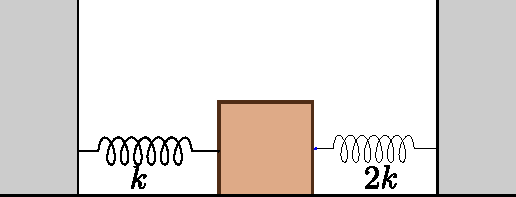
\includegraphics[scale=1.2]{p-6-1.pdf}
\caption{Schematizzazione del problema. \label{fig:4-p-6-1} }
\end{figure}

\subsubsection*{Soluzione}
Il problema è unidimensionale, perché tutte le forze che entrano in gioco sono dirette lungo uno stesso asse, che chiameremo $\hat{x}$. Di conseguenza la notazione vettoriale non è necessaria (ovvero: la scomposizione della seconda legge di Newton
$m \vec{a} =\sum_i \vec{F}_i$ è non banale solo lungo l'asse $\hat{x}$). 
Quando la massa si trova nel punto $x$ le forze agenti su di essa sono (Figura \ref{fig:4-p-6-2}): 
\begin{itemize}
\item la forza elastica data dalla prima molla (quella attaccata in $x=0$): $-kx$;
\item la forza elastica data dalla seconda molla (quella attaccata in $x=L$): $+2k(L-x)$;
\end{itemize}

 \begin{figure}[!ht]
 \centering
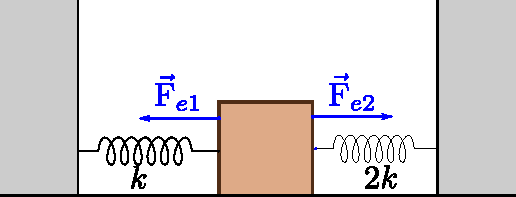
\includegraphics[scale=1.2]{p-6-2.pdf}
\caption{Diagramma delle forze agenti nel sistema.\label{fig:4-p-6-2} }
\end{figure}


Il primo segno (-) è stato messo notando che la coordinata $x$ è positiva, mentre la forza data dalla prima molla ha verso negativo. La seconda forza elastica ha invece verso positivo ed è proporzionale all'allungamento
$L-x_0$. Ricordiamo infatti che la forza applicata dalla molla, come per le funi, può solo tirare e non spingere. Se poniamo $x=x_0$ (posizione di equilibrio) allora la somma delle forza deve fare 0:
\begin{equation*}
-kx_0+ 2k(L-x_0)=0 
\end{equation*}
Ricaviamo quindi:
\begin{equation*}
-3kx_0+ 2kL=0 \quad \Rightarrow \quad x_0=\frac{L}{3}
\end{equation*}
Nell'istante in cui la molla a destra viene sganciata sulla massa agisce una sola forza , quella elastica data dalla
molla a sinistra, quindi: 
\begin{equation*}
F=-kx_0=-\frac{kL}{3}
\end{equation*}
Utilizzando la seconda legge di Newton:
\begin{equation*}
a=\frac{F}{m}=-\frac{kL}{3m}
\end{equation*}

\subsection{Dischi appesi \rstar \rstar}
La Figura \ref{fig:4-p-3-1} mostra la disposizione di 4 dischi appesi con delle funi. La fune più lunga passa da una carrucola priva di attrito ed è collegata al muro ed esercita una tensione $T=88.2\;\text{N}$. Le tensioni nei tre tratti di fune più brevi sono: $T_1=58.8\;\text{N}$, $T_2=39.2\;\text{N}$ e $T_3=24.5\;\text{N}$.

\begin{figure}[!ht]
\centering
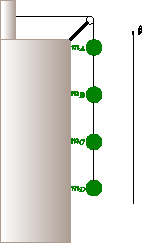
\includegraphics[scale=1.8]{p-3-1.pdf}
\caption{Illustrazione della situazione del problema.} 
\label{fig:4-p-3-1} 
\end{figure}

\subsubsection*{Soluzione}
Notiamo due fatti fondamentali alla soluzione del problema: nessun corpo è in movimento (quindi tutti i corpi hanno accelerazione 0) e le funi possono solo tirare e non spingere (quindi la tensione sarà applicata dall'oggetto verso il centro della fune). Conviene iniziare l'analisi corpo per corpo a partire dal disco D. In Figura  \ref{fig:4-p-3-2} il diagramma di corpo libero del sistema. 

\begin{figure}[!ht]
\centering
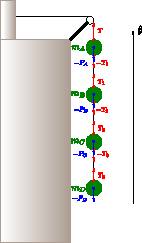
\includegraphics[scale=3]{p-3-2.pdf}
\caption{Diagramma di corpo libero con forze peso e tensioni.} 
\label{fig:4-p-3-2} 
\end{figure}

Scriviamo per il disco D la II legge di Newton esprimendola per coordinate supponendo l'asse $y$ rivolto verso l'alto ($\vec{\text{P}}_D$ è la forza peso):
%
\begin{gather*}
\vec{\text{P}}_D+\vec{\text{T}}_3=0 \quad \Longrightarrow \quad -P_D\hat{y}=-T_3\hat{y} \quad \Longrightarrow \quad -m_Dg\hat{y}=-T_3\hat{y}\\
m_D=\frac{T_3}{g} \quad \Longrightarrow \quad m_D=\frac{24.5\;\text{N}}{9.8\;\text{m/s}^2}=2.5\;\text{kg}
\end{gather*}
%
Adesso passiamo ad analizzare il disco C ottenendo una descrizione generale anche per i dischi B e A. La II legge di Newton si può quindi scrivere come:
%
\begin{gather*}
\vec{\text{P}}_C+\vec{\text{T}}_3+\vec{\text{T}}_2=0 \quad \Longrightarrow \quad (-P_C-T_3)\hat{y}=-T_2\hat{y} \quad \Longrightarrow \quad -m_Cg\hat{y}=(T_3-T_2)\hat{y}\\
m_C=\frac{T_2-T_3}{g} \quad \Longrightarrow \quad m_C=\frac{(30.2-24.5)\;\text{N}}{9.8\;\text{m/s}^2}=1.5\;\text{kg}
\end{gather*}
%
Similmente si ottiene:
%
\begin{gather*}
m_B=\frac{T_1-T_2}{g} \quad \Longrightarrow \quad m_B=\frac{(58.8-39.2)\;\text{N}}{9.8\;\text{m/s}^2}=2\;\text{kg} \\
m_A=\frac{T-T_1}{g} \quad \Longrightarrow \quad m_A=\frac{(88.2-58.8)\;\text{N}}{9.8\;\text{m/s}^2}=3\;\text{kg}
\end{gather*}
%

\subsection{Trainare due casse in presenza di attrito \rstar \rstar}
Due casse connesse da una fune sono trascinate da una forza  orizzontale $F=70\;\text{N}$, supponiamo $m_1=10\;\text{kg}$ e $m_2=19\;\text{kg}$ e il coefficiente di attrito dinamico valga 0.15. Determinare la tensione $T$ della fune e l'accelerazione del sistema. La situazione è riassunta in Figura \ref{fig:4-p-4-1}.

\begin{figure}[!ht]
\centering
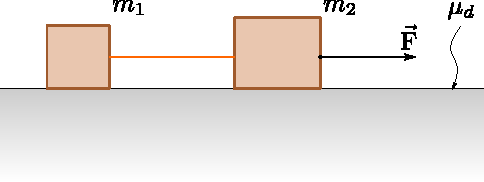
\includegraphics[scale=1]{p-4-1.pdf}
\caption{Due casse collegata da una fune e trascinate.} 
\label{fig:4-p-4-1} 
\end{figure}

\subsubsection*{Soluzione}
Notiamo subito che l'accelerazione delle due casse deve essere la stessa in quanto la corda è inestensibile: se fosse $a_2>a_1$ allora la corda si spezzerebbe, mentre avere $a_1>a_2$ è impossibile perché vorrebbe dire una fune non tesa, incapace di esercitare la tensione (e quindi l'unica forza che tira $m_1$). Riportiamo in Figura \ref{fig:4-p-4-2} il diagramma di corpo libero delle masse.

\begin{figure}[!ht]
\centering
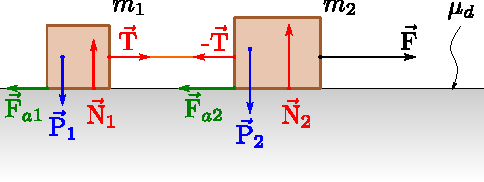
\includegraphics[scale=1]{p-4-2.pdf}
\caption{Diagramma di corpo libero delle masse in gioco.} 
\label{fig:4-p-4-2} 
\end{figure}

Conviene iniziare l'analisi da $m_1$ per cui scriviamo la II legge di Newton:
%
\begin{gather*}
\vec{\text{F}}_{a1}+\vec{\text{N}}_1+\vec{\text{P}}_1+\vec{\text{T}}=m_1\vec{a}
\end{gather*}
%
Imponiamo l'equilibrio verticale ($a_y=0$):
%
\begin{gather}
N_1-P_1=0 \quad	\Longrightarrow \quad N_1=P_1=m_1g
\label{eq:4-p-4-1} 
\end{gather}
%
La scomposizione lungo la componente orizzontale darà invece:
%
\begin{gather}
-F_{a1}+T=m_1a \quad	\Longrightarrow \quad T=F_{a1}+m_1a
\label{eq:4-p-4-2} 
\end{gather}
%

Passiamo adesso all'analisi di $m_2$, scriviamo sempre la II legge di Newton:
%
\begin{gather*}
\vec{\text{F}}+\vec{\text{F}}_{a2}+\vec{\text{N}}_2+\vec{\text{P}}_2-\vec{\text{T}}=m_2\vec{a}
\end{gather*}
%
Anche in questo caso imponiamo l'equilibrio verticale:
%
\begin{gather}
N_2-P_2=0 \quad	\Longrightarrow \quad N_2=P_2=m_2g
\label{eq:4-p-4-3} 
\end{gather}
%
Ed infine scriviamo la componente orizzontale dell'equazione della II legge di Newton.
%
\begin{gather}
-T-F_{a2}+F=m_2a
\label{eq:4-p-4-4} 
\end{gather}
%
Ricordiamo che la forza di attrito dinamico vale $F_a=\mu_dN$, sostituendo le eqq. \ref{eq:4-p-4-1}-\ref{eq:4-p-4-2}-\ref{eq:4-p-4-3} in eq. \ref{eq:4-p-4-4} otteniamo:
%
\begin{gather*}
-(F_{a1}+m_1a)-F_{a2}+F=m_2a \quad	\Longrightarrow \quad a= \frac{F-F_{a1}-F_{a2}}{m_1+m_2}=\frac{F-\mu_dg(m_1+m_2)}{m_1+m_2}
\end{gather*}
%
Con i dati forniti nel testo abbiamo:
%
\begin{gather*}
a=\frac{70\;\text{N}-0.15 \cdot 9.8\;\text{m/s}^2(10\;\text{kg}+19\;\text{kg})}{10\;\text{kg}+19\;\text{kg}}\approx 0.94 \frac{\text{m}}{\text{s}^2}
\end{gather*}
%
Possiamo quindi ricavare la tensione dall'eq. \ref{eq:4-p-4-2}:
%
\begin{gather*}
T=m_1(g\mu_d+a) \quad \Longrightarrow \quad T=10\;\text{kg} \; \qty(0.15 \cdot 9.8 \;\frac{\text{m}}{\text{s}^2} + 0.94\;\frac{\text{m}}{\text{s}^2})\approx 24\;\text{N}
\end{gather*}
%

\subsection{Molla, masse ed attrito  \rstar \rstar}
Due masse $m_1$ e $m_2$ su un piano orizzontale sono collegate tra loro da una molla di lunghezza a riposo nulla e costante elastica $k$. Determinare la massima distanza a cui le masse possono rimanere in equilibrio in presenza di un attrito statico con coefficiente $\mu_s$.

\subsubsection*{Soluzione}
Mettiamoci nel sistema di riferimento cartesiano che ha come asse $\hat{y}$ quello verticale ($\vec{g}=-g\hat{y}$) e come asse $\hat{x}$ la retta congiungente le due masse $m_1$ e $m_2$. 
Le forze agenti sono riportate in Figura \ref{fig:4-p-5}), notiamo che i versi delle forze elastiche sono verso il centro della molla, sempre per il fatto che essa può tirare e non spingere. Le forze di attrito si oppongono allo spostamento quindi saranno in verso opposto rispetto alle forze elastiche. Visto che assumiamo una molla di massa nulla i moduli delle forze elastiche saranno gli stessi.

\begin{figure}[!ht]
\centering
\includegraphics[scale=1.2]{p-5.pdf}
\caption{Diagramma delle forze agenti nel sistema.\label{fig:4-p-5} }
\end{figure}

Come al solito si procede scrivendo la seconda legge di Newton $m \vec{a} =\sum_i \vec{F}_i$ scomposta nel
sistema di riferimento cartesiano scelto. Dato che vogliamo che le masse siano in equilibrio, dovrà valere, per 
ciascuna delle due masse, $\vec{a}=0$ e quindi: $\sum_i \vec{F}_i=0$. 

Cominciamo con lo scomporre lungo l'asse $\hat{y}$ le forze agenti su $m_1$,
imponendo che la somma delle componenti di tale forze sia nulla: 
\begin{equation*}
-m_1 g + N_1=0 \quad \Longrightarrow \quad N_1=m_1 g
\end{equation*}
Similmente possiamo trovare $N_2$: 
\begin{equation*}
-m_2 g + N_2=0 \quad \Longrightarrow \quad N_2=m_2 g
\end{equation*}
Le forze di attrito statico devono \textit{sempre} rispettare il vincolo:
\begin{equation*}
F_{1A} \leq \mu_s R_1 = \mu_s m_1 g
\end{equation*}
e:
\begin{equation*}
F_{2A} \leq \mu_s R_2 = \mu_s m_2 g
\end{equation*}

Ora scomponiamo lungo l'asse $\hat{x}$ le forze agenti su $m_1$ e $m_2$,
imponendo che la somma di tali componenti faccia $0$: 
\begin{gather*}
-F_{1A}+kL=0\\
+F_{2A}-kL=0
\end{gather*}
dove $L$ indica la distanza fra le due masse. Si sono riscritte le due forze $F_{1e}$, $F_{2e}$ utilizzando
la legge $F_e=k\Delta x$. Possiamo quindi scrivere:
\begin{gather*}
L=\frac{F_{1A}}{k} \leq \frac{\mu_s m_1 g}{k}\\
L=\frac{F_{2A}}{k} \leq \frac{\mu_s m_2 g}{k}\\
\end{gather*}
Abbiamo ottenuto due disuguaglianze su $L$. Quella più "stringente" è quella che corrisponde a un valore minore della massa $m$. In definitiva: 
\begin{gather*}
L_{max}=\frac{\mu_s \cdot \text{min}(m_1,m_2)\cdot g}{k}\\
\end{gather*}

\chapter{Lavoro e Conservazione dell'Energia}
\section{Esercizi}

\subsection*{Esercizio 1}
A temperatura ambiente una molecola di ossigeno di massa $5.31\times 10^{-26}\;$kg ha mediamente un'energia cinetica  $K=6.21\times 10^{-21}\;$J. Con che velocità si muove?

\subsubsection*{Soluzione}
Ricordando la formula dell'energia cinetica:
\begin{equation*}
K=\frac{1}{2}mv^{2},
\end{equation*}
possiamo dire che:
\begin{equation*}
v=\sqrt{\frac{2K}{m}}=\sqrt{\frac{2\cdot 6.21\times 10^{-21}\, \text{J}}{5.31\times 10^{-26}\text{kg}}}=484\; \text{m}/\text{s}
\end{equation*}

\subsection*{Esercizio 2}
(a) Se l'energia cinetica di un'auto viene raddoppiata, di quanto aumenta la sua velocita?\\
(b) Se fosse invece la velocità a raddoppiare, di quanto crescerebbe l'energia cinetica dell'auto?\\
(c) Che lavoro è necessario per fermare un'auto di $1250\;$ kg che viaggia a $105\;$ km/h?

\subsubsection*{Soluzione}
(a) Siano $K_{1}$ e $K_{2}$ energie cinetiche, $K_{2}$ il doppio di $K_{1}$. Dunque avremo:
\begin{equation*}
K_1=\frac{1}{2}mv_{1}^{2}  \; , \;   K_2=\frac{1}{2}mv_{2}^{2}=2K_{1}=m v_{1}^{2}\, \, \,  \Rightarrow \, \, \,  v_{2}^{2}= 2 v_{1}^{2}
\end{equation*}
Dunque: $v_{2}=\sqrt{2}v_{1}$.Ovviamente $v_2$ e $v_1$ sono i moduli dei vettori velocità. \\

(b) Utilizzando un ragionamento analogo a quello del punto (a) e ponendo stavolta $v_{2}=2 v_{1}$, troviamo: $K_{2}=4 K_{1}$.\\

(c) La quantità di lavoro $W$ necessario per fermare l'auto sarà quello che eguaglierà la sua energia cinetica: $K=1/2m v^2$. Il segno del lavoro sarà negativo in quanto la direzione di moto della macchina è opposta alla direzione della forza che la frena. Dunque:
\begin{equation*}
W=-\frac{1}{2}m v^{2}=-\frac{1}{2}\times 1250\; \text{kg}  \left (29.1 \text{m}/\text{s} \right)^2=-529.256\; \text{kJ}.
\end{equation*}

\subsection*{Esercizio 3}
Un pilota cade per $H=370\;$m dopo essere saltato dal suo aeroplano, senza che il paracadute si sia aperto. Atterra su un cumulo di neve, creando un cratere profondo $h=1.1\;$m, sopravvivendo. Assumendo che la massa del paracadutista sia $m=78\;$ kg e che la sua velocità di impatto con la neve sia $v_{0}=35\;$ m/s, trovare:\\
(a)Il lavolo compiuto dalla neve nel fermare il pilota.\\
(b)La forza media esercitata dalla neve sul pilota.\\
(c)Il lavoro compiuta dalla resistenza del l'aria sul pilota durante la caduta.

\subsubsection*{Soluzione}
(a) Come nel problema precedente, possiamo dire che il lavoro compiuto dalla forza applicata dalla neve sarà uguale all'energia cinetica dissipata durante l'impatto. Quindi:
\begin{equation*}
W_{neve}=-\frac{1}{2}\; 78\; \text{kg} \times \left (35\; \frac{\text{m}}{\text{s}}\right )^{2}\simeq  -47.77\; \text{kJ}
\end{equation*}
(b) Sappiamo che il lavoro è definito anche come forza per spostamento. Essendoci ricavati il lavoro nel punto (a), e sapendo che lo spostamento è di $\Delta=1.1 \,$m, possiamo trovare la forza F:
\begin{equation*}
F=\frac{W}{\Delta}=\frac{-47.775\; \text{kJ}}{1.1 \; \text{m}}=-43\;\text{kN}
\end{equation*}
(c) Se non avessimo considerato la reistenza dell'aria, la velocità $v_{1}$ del pilota prima di colpire il cumulo di neve sarebbe quella raggiunta sotto l'effetto dell'accelerazione di gravità $\vec{g}$, nei $370\;m$ di volo. Possiamo trovare $v_{1}$ utilizzando la conservazione dell'energia:
\begin{equation*}
mgh=\frac{1}{2}mv_{1}^{2} \qquad \Rightarrow \qquad v_{1}=\sqrt{2 g h}=\sqrt{2\cdot 9.81\;\frac{\text{m}}{\text{s}} \; 370\; \text{m} }\simeq 85 \; \frac{\text{m}}{\text{s}}
\end{equation*} 
$v_{1}$ differisce dalla velocità data dal testo del problema, la differenza fra le due velocità è dovuta al fatto che il testo del problema considera che il pilota sia frenato, nella caduta, dall'attrito dell'aria. Il lavoro compiuto da questo attrito sarà uguale all'energia cinetica mancante rispetto al caso in cui non si consideri la resistenza dell'aria. Dunque:
\begin{equation*}
W_{aria}= \frac{1}{2}m\left( v_{0}^{2}- v_{1}^{2} \right )= -234\; \text{kJ}
\end{equation*}


\subsection*{Esercizio 4}
Il cavo di un ascensore si spezza quando la cabina di massa $M=920 \;\text{kg}$ si trova a $h=28\; m$ al di sopra di un'enorme molla di costante elastica $k=2.2\cdot 10^{5}\; \text{N}/m$ posizionata in fondo alla tromba dell'ascensore. Calcolare: (a) il lavoro compiuto dalla forza peso sull'ascensore prima che colpisca la molla; (b) la velocità dell'ascensore appena prima di colpire la molla; (c) di quanto la molla si comprime.

\subsubsection*{Soluzione}
(a) La forza peso e il vettore spostamento dell'ascensore durante la caduta sono allineati (paralleli). Dunque il $\cos$ dell'angolo compreso è $\cos 0=1$ e il lavoro compiuto dalla forza peso è semplicemente:
\begin{equation*}
W_{g}= F_{g} h= mg h \simeq (920 \;\text{kg})(9.81\; \frac{\text{m}}{\text{s}^2})(28\; \text{m}) \simeq 252.45 \; \text{kJ}
\end{equation*}
(b) Le forze agenti sull'ascensore durante il moto (caduta+rallentamento sulla molla) sono: forza peso, forza elastica. Entrambe sono di tipo \textit{conservativo}. Vale quindi il \textit{teorema di conservazione dell'energia meccanica}.
Conviene utilizzare come istante iniziale quello di inizio della caduta e come istante finale quello dove l'ascensore tocca la molla. 
Avremo allora:
\begin{equation*}
E_{f}=E_{i} \qquad  \Rightarrow \qquad mgh=\frac{1}{2} m v_{f}^2
\end{equation*}
da cui:
\begin{equation*}
v_{f}=\sqrt{2gh}\simeq\sqrt{2\cdot 9.81\; \frac{\text{m}}{\text{s}^2}\cdot 28\; \text{m}} \simeq 23.4 \; \frac{\text{m}}{\text{s}}
\end{equation*}
(c) Per trovare la compressione $\Delta$ della molla possiamo di nuovo applicare la conservazione dell'energia meccanica.
Conviene utilizzare come istante iniziale quello di inizio della caduta e come istante finale quello dove la caduta dell'ascensore termina, alla fine della fase di compressione della molla. Posizionando lo $0$ dell'asse $y$ (lungo il quale avviene il moto) 
nel punto di arrivo finale dell'ascensore, avremo che la posizione iniziale dell'ascensore è ad altezza $\Delta + h$, quindi:
\begin{equation*}
E_{f}=E_{i} \qquad  \Rightarrow \qquad mg(h+\Delta)=\frac{1}{2}k \Delta^{2} 
\end{equation*}
(L'energia potenziale finale è 0). Si ottiene:
\begin{equation*}
\Delta^2-\frac{2mg}{k}\Delta-\frac{2mgh}{k}\qquad \Rightarrow \qquad \Delta=\frac{1}{2}\left(\frac{2mg}{k}\pm\sqrt{4\frac{(mg)^2}{k^2}-4\left(-\frac{mv^2}{k}\right)}\right)
\end{equation*}
Quindi, inserendo i valori numerici, troviano $\Delta=1.56\;m$. 

\subsection*{Esercizio 5}
In una centrale idroelettrica, l'acqua fluisce da una diga con velocità iniziale $v\simeq 0$ e con un flusso di $650\; \text{kg}/$s cade verticalmente per $h= 81\; m$ prima di colpire le pale di una turbina. Calcolare: (a) la velocità dell'acqua appena prima di colpire le pale della turbina (trascurando la resistenza dell'aria); (b) la potenza ricavata dal sistema assumendo un'efficienza $\eta =58\; \%$ per il trasferimento di energia alle turbine. 

\subsubsection*{Soluzione}
(a) La conservazione dell'energia meccanica per un elemento di acqua di massa $m$ si scrive:
\begin{equation*}
E_{i}=E_{f} \qquad  \Rightarrow \qquad mgh=\frac{1}{2} m v^2
\end{equation*}
da cui:
\begin{equation*}
v=\sqrt{2gh}=40\; \frac{\text{m}}{\text{s}^2}
\end{equation*}
(b) Il sistema ``assorbe'' parte dell'energia cinetica incorporata dall'acqua durante la caduta. L'energia cinetica ``disponibile'' per unità di tempo sarà:
\begin{equation*}
W= \frac{1}{2}\;650 \; \frac{\text{kg}}{\text{s}} \cdot \left( 40\; \frac{\text{m}}{\text{s}^2}\right)^2=5.2\times 10^5\; \frac{\text{J}}{\text{s}}
\end{equation*}
e quindi la potenza trasferita sarà:
\begin{equation*}
P=0.58 W = 5.2\times 10^5\; \text{W}
\end{equation*}


\subsection*{Esercizio 6}
Un biscotto ha un valore energetico $E=54 \,$kcal. Ricordiamo che $1 \, \text{kcal} \simeq 4.18 \, \cdot 10^3 \, \text{J}$. $E$
corrisponde all'energia che il nostro corpo riesce a ``estrarre'' dal biscotto, trasformando l'energia chimica presente nei suoi componenti chimici in altre forme di energia (termica o cinetica).  Assumendo che il corpo umano trasformi completamente in lavoro l'energia del cibo: 
(a) quanto in alto potrebbe salire su una scala un uomo di massa $m=80 \, \text{kg}$ utilizzando l'energia $E$? (b) Se quell'uomo saltasse giù dalla scala, quale sarebbe la velocità con cui raggiungerebbe il suolo?

\subsubsection*{Soluzione}
(a) Si ha:
\begin{equation*}
E= 54 \, \text{kcal} \simeq  54 \cdot 4.18 \cdot 10^3 \text{J} \simeq 2.25  \cdot 10^5 \text{J}
\end{equation*}
Ponendo uguale quest'energia all'energia potenziale dell'uomo quando si trova ad un'altezza $h$ dal suolo, si ha:
\begin{equation*}
E=mgh \qquad \Rightarrow \qquad h=\frac{E}{mg}\simeq 288 \, \text{m}
\end{equation*}
(b) Utilizzando la conservazione dell'energia meccanica si ottiene subito:
$v=\sqrt{2gh}\simeq 75 \;\frac{\text{m}}{\text{s}}= 270 \;\frac{\text{km}}{\text{h}}$

\subsection*{Esercizio 7}
Un ciclista, senza pedalare né frenare, scende per una collina di pendenza $\theta=7.0^{\circ}$ a una velocità costante di $v_{0}=5.0\;\frac{\text{m}}{\text{s}}$. Assumendo una massa complessiva (ciclista e bicicletta) pari a $m=75\; \text{kg}$ quale potenza deve sviluppare il ciclista per essere in grado di risalire la stessa collina alla stessa velocità?\\
\textit{Suggerimento}: in una discesa la componente parallela alla strada della forza di gravità è opposta in verso alla forza di attrito. Invece in una salita, entrambe le forze hanno lo stesso verso! 

\subsubsection*{Soluzione}
Visto che il ciclista durante la discesa né frena né pedala, le forze in gioco sono solo l'attrito e la gravità. Essendo la velocità di discesa costante, l'accelerazione del ciclista deve essere nulla, questo vuol dire che la forza di attrito bilancia quella di gravità:
\begin{equation*}
F_{attrito}=mg \sin(\theta)=mg\sin(\theta) \simeq 90 \; \text{N}
\end{equation*}
Per risalire la collina con la stessa velocità, il ciclista dovrà applicare una forza $F_{ciclista}$ che bilanci sia la forza id gravità, sia la forza di attrito (questo perché la velocità deve esser anche in questo caso costante, e quindi deve essere nulla la sommatoria delle forze agenti sulla bicicletta). Si avrà dunque:
\begin{equation*}
F_{ciclista}=F_{attrito}+ mg \sin(\theta)=2\; mg\sin(\theta)\simeq 180 \; \text{N}
\end{equation*}
Dalla definizione di potenza dunque possiamo ricavare:
\begin{equation*}
P_{ciclista}=F_{ciclista}\cdot v_{0} \simeq 180\; \text{N} \cdot 5.0\; \frac{m}{s}= 900\; W. 
\end{equation*}

\subsection*{Esercizio 8}
Un blocco di legno di massa $m=0.62\; \text{kg}$ si trova su un tavolo ed è saldamente attaccato ad una molla ($k=180\; \text{N}/\text{m}$) di massa trascurabile che lo collega orizzontalmente ad una parete. Quando si comprime la molla di $l_0=5.0\; cm$ e poi si rilascia, il blocco supera la posizione di equilibrio di $l_1=2.3\;cm$ prima di fermarsi e tornare indietro. Qual è il coefficiente di attrito dinamico tra il blocco e il tavolo?

\subsubsection*{Soluzione}
Se non ci fosse attrito, la molla dovrebbe oscillare in modo simmetrico rispetto alla posizione di equilibrio e quindi il blocco dovrebbe fermarsi $5.0\; cm$ dopo la posizione di equilibrio, e poi tornare indietro. La presenza dell'attrito fa sì che parte dell'energia del blocca venga dissipata (in calore) e dunque l'estensione della molla alla prima oscillazione di riduce (in questo caso a $l_1=2.3\;cm$). In altre parole la forza di attrito compie un lavoro che è pari alla differenza di energia meccanica 
della massa fra l'inizio e la fine del moto:
\begin{equation*}
\mathcal{L}
_{attrito}=\frac{1}{2}k(l_1^2-l_0^2)=-0.2\; J
\end{equation*}
Dalla definizione di lavoro possiamo ricavare la forza d'attrito dinamico agente sul blocco (il vettore sposamento 
e il vettore forza in questo caso sono paralleli):
\begin{equation*}
\mathcal{L}
_{attrito}=F_{attrito} (l_0+l_1)\qquad  \Rightarrow \qquad F_{attrito}=\frac{\mathcal{L}
_{attrito}}{(l_0+l_1)} \simeq -2.43 \; \text{N}
\end{equation*}
D'altra parte ricordiamo che per l'attrito dinamico vale:
\begin{equation*}
F_{attrito}=\mu_{d}\cdot F_{normale}=\mu_{d}  mg \qquad  \Rightarrow \qquad \mu_{d} mg=-2.43\; \text{N}
\end{equation*}
e quindi:
\begin{equation*}
\mu_{d}\simeq 0.4
\end{equation*}

\subsection*{Esercizio 9}
Un pianoforte di massa $M=100 \;kg$ viene caricato su un camion con una rampa lunga $d=3\; m$ e inclinata di $\alpha=30^{\circ}$, spingendolo verso l'alto con una forza $\vec{F}$ di modulo $F=1000 \; N$ parallela al piano. Quale sarà il lavoro compiuto dalla forza applicata e della forza peso al termine dell'operazione? Arrivato a destinazione, il pianoforte viene lasciato scivolare fino a terra su un'altra rampa, inclinata di $\gamma=45^{\circ}$. Quale sarà il lavoro fatto dalla forza peso durante la discesa? Quale risulta quindi il lavoro totale fatto dalla forza peso nel trasloco?

\subsubsection*{Soluzione}

La forza applicata è per ipotesi parallela al piano e quindi allo spostamento del pianoforte. Il lavoro compiuto sarà percio semplicemente:\\
\begin{equation*}
\mathcal{L}
_F =  \vec{F} \cdot \vec{d} = Fd \cos \theta = Fd= 1000 \cdot 3 \, \text{J} = 3000 \, \text{J}
\end{equation*}
($\vec{d}$ è il vettore spostamento).  Per calcolare il lavoro compiuto dalla forza peso, dobbiamo calcolare la componente della forza lungo la direzione del moto. Orientando l'asse $x$ parallelamente al piano, in modo che la direzione positiva sia verso la salita, otteniamo che la componente della forza peso che ci interessa è $P_{//} = -M g \sin\alpha$. Il segno meno è dovuto al fatto che la componente della forza peso parallela al piano è diretta verso il basso. Allora, il lavoro compiuto dalla gravità sarà pari a:\\
\begin{equation*}
\mathcal{L}
_G = \vec{P} \cdot \vec{d} =P_{//} d= -Mg d \sin\alpha \simeq  -1470 \, \text{J}
\end{equation*}\\

Infine, vogliamo calcolare il lavoro fatto dalla forza peso nella discesa. Cominciamo col calcolare quanto vale la lunghezza $d'$ della seconda rampa, imponendo che l'altezza da terra $h$ della cima risulti la stessa raggiunta con la prima rampa:\\
\begin{equation*}
h=d \sin\alpha = d' \sin\gamma \qquad \Rightarrow  \qquad d' = \frac{\sin\alpha}{\sin\gamma} \ d = \frac{1/2}{\sqrt{2}/2} \: 3 \; \text{m} = \frac{1}{\sqrt{2}} \: 3 \; m \approx 2.12 \; \text{m}
\end{equation*}\\
Utilizzando lo stesso metodo visto prima, possiamo allora calcolare il lavoro compiuto dalla forza peso in questo secondo tragitto (stavolta la componente parallela al piano e lo spostamento sono diretti nello stesso verso: il lavoro sarà positivo!):\\
\begin{equation*}
\mathcal{L}
'_G = P_{//} d' = M g d' \sin\gamma = 100 \cdot 9.81 \cdot \frac{1}{\sqrt{2}} \cdot 2.12 \text{J} = 1470 \; \text{J}
\end{equation*}
Il lavoro totale compiuto dalla forza peso sarà perciò:\\
\begin{equation*}
\mathcal{L}
_{G_{tot}}= \mathcal{L}
_G + \mathcal{L}
'_G = (-1470 + 1470) \; J = 0 \; J
\end{equation*}\\

Il lavoro totale è nullo. Questo risultato era atteso perchè, essendo la gravità una \textit{forza conservativa}, il lavoro da essa compiuto dipende solo dalla \textit{differenza di quota del corpo} (quota raggiunta alla fine del moto meno quota iniziale). Ma dato che il pianoforte è partito dal suolo ed è arrivato nuovamente al suolo, la differenza di quota è nulla, e con essa il lavoro.\\

\subsection*{Esercizio 10}
Un traslocatore vuole trasportare una cassa di massa $m=50 \;$ kg in cima ad un piano inclinato su cui è presente attrito dinamico ($\mu_d = 0.2$). Per farlo tira la cassa con una fune inestensibile, applicando una forza $\vec{F}$ costante, parallela al piano e di modulo $F=100 \;$ N . Sapendo che la cima del piano inclinato sta ad un'altezza $h=2 \;$ m dal suolo e che l'inclinazione del piano è $\alpha=30^{\circ}$, calcolare il lavoro compiuto dal traslocatore, dalla forza di attrito e dalla forza peso quando la cassa è arrivata in cima.

\subsubsection*{Soluzione}
Per calcolare il lavoro effettuato dal traslocatore, è necessario conoscere la lunghezza $L$ della rampa. Possiamo ottenerla tramite $h$ ed $\alpha$. Infatti: 
\begin{equation*}
h=L \sin\alpha \Longrightarrow L = \frac{h}{\sin\alpha} = \frac{2}{1/2} \; \text{m} = 4 \; \text{m}
\end{equation*}
Allora, dato che $\vec{F}$ è diretta parallelamente al piano, il lavoro compiuto dal traslocatore nel tirare la cassa sarà:
\begin{equation*}
\mathcal{L}
_T = \vec{F} \cdot \vec{d} = FL = 100 \cdot 4 \; \text{J} = 400 \; \text{J}
\end{equation*}\\
dove $\vec{d}$ è il vettore spostamento (parallelo a $\vec{F}$ e di modulo $L$). 
Il lavoro compiuto dalla forza di attrito, essendo anch'essa diretta parallelamente al piano (ma in direzione opposta al moto), sarà semplicemente dato da:\\
\begin{equation*}
\mathcal{L}
_{\text{attr}} =  \vec{F_{\text{attr}}} \cdot \vec{d} = - \mu_d m g L \cos\alpha  = - 0.2 \cdot 50 \cdot 10 \cdot \frac{\sqrt{3}}{2} \cdot 4 \; \text{J} \approx - 346 \; \text{J}
\end{equation*}
Infine, per calcolare il lavoro della forza peso, essendo essa conservativa, possiamo eguagliare il lavoro compiuto all'opposto della variazione di energia potenziale gravitazionale:\\
\begin{equation*}
\mathcal{L}
_G = - \Delta U_G = -m g (h_{f} - h_{i}) = -mgh = - (50\cdot 10 \cdot 2) \; \text{J}= -1000 \; \text{J}
\end{equation*}\\

\subsection*{Esercizio 11}
Uno sciatore di massa $M=50 \;$ kg affronta una discesa libera, lunga $L=160 \; m$, di pendenza costante $\alpha=30^{\circ}$. Con che velocità attraverserà il traguardo se l'attrito tra sci e neve è trascurabile? Appena attraversato il traguardo, l'atleta mette di traverso gli sci per frenare, in un tratto orizzontale. Quale dev'essere il coefficiente di attrito tra gli sci e la neve perché lo sciatore si fermi in $d=100 \; m$? 

\subsubsection*{Soluzione}
Durante la discesa, possiamo assumere che l'unica forza che agisce sullo sciatore sia quella gravitazionale. Essendo conservativa, l'energia meccanica dello sciatore si conserva. Cominciamo allora a calcolare a quale quota $h$ si trovi lo sciatore al momento della sua partenza:\\
\begin{equation*}
h=L \sin\alpha = 160 \frac{1}{2} \; \text{m} = 80 \; \text{m}
\end{equation*}\\

Applichiamo ora il \textit{teorema di conservazione dell'energia} fra l'istante iniziale (nel quale lo sciatore si trova fermo ad un'altezza $h$ dal suolo) e l'istante finale dell'attraversamento del traguardo (in cui lo sciatore si muove ed è ad altezza $0$):
\begin{equation*}
E_{f}=E_{i} \qquad  \Rightarrow \qquad   \frac{1}{2} M v^2 = Mgh \qquad \Rightarrow \qquad v= \sqrt{2gh} = \sqrt{2\cdot 10 \cdot 80} \; \frac{\text{m}}{\text{s}} = 40 \;\frac{\text{m}}{\text{s}} 
\end{equation*}
Dal momento in cui inizia a frenare, sullo sciatore agisce la forza di attrito, che effettuerà un lavoro sullo sciatore. 
Il lavoro esercitato dalla forza di attrito è uguale alla variazione di energia cinetica dello sciatore, ovvero:
\begin{equation*}
\mathcal{L}
_{\text{attr}}= \Delta K = K_{f}-K_{i} = 0-K_{i} = -\frac{1}{2}Mv^2
\end{equation*}
Si ha: $\mathcal{L}
_{attr} = -F_{attr} d = -\mu_d M g d$. Possiamo allora ricavare $\mu_d$:\\
\begin{equation*}
\mu_d M g d = \frac{1}{2}M v^2 \qquad \Longrightarrow  \qquad \mu_d = \frac{v^2}{2 g d} = \frac{1600}{2\cdot 10 \cdot 100} = 0.8
\end{equation*}\\

\subsection*{Esercizio 12}
Supponiamo di lasciar cadere un vaso da un terrazzo ad un'altezza $h=20\; m$ dal suolo. Quale sarà la velocità con cui tocca il marciapiede? Sul marciapiede è posto un tappeto elastico, schematizzabile come una molla di costante elastica $k=800 \;$N/m e lunghezza a riposo nulla. Se il vaso ha una massa $m=500 \;$ g, quanto vale la deformazione massima subita dal tappeto? Qual è la velocità del vaso nel momento in cui la deformazione del tappeto è la metà di quella massima?

\subsubsection*{Soluzione}
Durante la caduta, l'unica forza che agisce sul vaso è la forza peso $\vec{P}$. Essendo essa di tipo \textit{conservativo}, l'energia meccanica del sistema si conserva. Applichiamo allora il \textit{teorema di conservazione dell'energia meccanica} fra l'istante iniziale (quello in cui il vaso viene lasciato cadere, da fermo, da un'altezza $h$ dal suolo) e quello finale (il momento dell'impatto al suolo). Avremo:\\
\begin{equation*}
E_{i}=E_{f} \qquad  \Rightarrow \qquad  mgh= \frac{1}{2}m v^2  \qquad  \Rightarrow \qquad v= \sqrt{2gh} = \sqrt{2\cdot 10 \cdot 20} \; \frac{\text{m}}{\text{s}} = 20 \; \frac{\text{m}}{\text{s}}
\end{equation*}
Consideriamo il caso in cui sul marciapiede sia presente il tappeto elastico. Anche la forza elastica è conservativa, quindi anche in questo caso possiamo applicare il teorema di conservazione dell'energia. Il momento di massima deformazione del tappeto coincide con quello in cui il vaso si ferma a causa dell'opposizione del tessuto elastico:
se infatti il vaso avesse ancora una velocità non nulla all'istante di tempo successivo il tappeto sarebbe ancor più deformato. Possiamo allora calcolare la deformazione massima $d_{max}$ in modo analogo al precedente. L'istante finale coinciderà con quello in cui il corpo si ferma, e sarà presente solo energia potenziale elastica:\\
\begin{equation*}
E_{i}=E_{f} \quad  \Rightarrow \quad  mgh = \frac{1}{2}k d_{max}^2 \quad  \Rightarrow \quad d_{max}= \sqrt{\frac{2mgh}{k}} = \sqrt{\frac{2\cdot 0.5 \cdot 10 \cdot 20 }{800}} \; \text{m} = \sqrt{\frac{1}{4}}  \; \text{m} = 0.5 \; \text{m}
\end{equation*}
Rispondiamo infine all'ultima domanda. In questo caso l'istante finale coincide con il momento in cui la deformazione del tappeto è esattamente la metà di $d_{max}$: avremo in questo istante sia energia potenziale elastica che cinetica. Chiamiamo $v_1$ la velocità cercata. Avremo:\\
\begin{equation*}
E_{i}=E_{f} \qquad  \Rightarrow \qquad  mgh = \frac{1}{2}m v_1^2 + \frac{1}{2}k \left(\frac{d_{max}}{2}\right)^2 \qquad  \Rightarrow \qquad  \frac{1}{2}m v_1^2 = mgh - \frac{1}{2}k\frac{d_{max}^2}{4}
\end{equation*}
che è un'equazione per l'incognita $v_1$. Troviamo:
\begin{equation*}
v_1 = \sqrt{2gh-\frac{k d^2_{max}}{4m}} \approx 17.32 \; \frac{\text{m}}{\text{s}}
\end{equation*}

\subsection*{Esercizio 13}
Una scatola di massa $M=10 \; kg$ è poggiata su un piano inclinato di $\alpha=30^{\circ}$ ad un'altezza $h_0=1\;$m da terra. Viene lasciata libera di scendere, senza attrito. Che velocità avrà in fondo al piano? A questo
punto la scatola comincia a risalire un secondo piano inclinato di $\beta=45^{\circ}$. A che altezza si fermerà? Come cambiano le risposte se sui piani è presente attrito dinamico descritto da $\mu_d = 0.1$?

\subsubsection*{Soluzione}
In assenza di attrito, l'unica forza che compie lavoro sulla scatola è la forza peso $\vec{P}$, che è di tipo conservativo. Quindi l'energia meccanica del sistema si conserva. Possiamo applicare il \textit{teorema di conservazione dell'energia} per rispondere alle prime due domande.
\begin{itemize}
\item  Per calcolare la velocità alla fine del piano, eguagliamo l'energia meccanica all'istante di tempo iniziale, ovvero quando la scatola comincia, da ferma, la discesa, a quella del momento finale, quando la scatola arriva in fondo al piano:
\begin{equation*}
E_{i}=E_{f} \qquad  \Rightarrow \qquad   Mgh_0 = \frac{1}{2}M v^2 \qquad  \Rightarrow \qquad v=\sqrt{2gh_0}= \sqrt{2\cdot 9.81 \cdot 1} \;\frac{\text{m}}{\text{s}} \approx 4.43 \; \frac{\text{m}}{\text{s}}
\end{equation*}\\

\item Per calcolare l'altezza finale utilizziamo lo stesso metodo. Abbiamo due possibili scelte per l'istante iniziale: 
a) l'istante in cui la scatola comincia la salita del secondo piano inclinato, con velocità $v$ appena calcolata; b) l'istante in cui la scatola comincia la discesa del primo piano inclinata, da ferma e dall'altezza $h_0$. 
Le due scelte sono del tutto equivalenti. Seguendo la strada b) troviamo:
\begin{equation*}
E_{i}=E_{f} \qquad  \Rightarrow \qquad   Mgh_0 = Mg h_{f} \qquad  \Rightarrow \qquad    h_{f}=h_0= 1\; \text{m}
\end{equation*}
Verificate che anche con scelta a) dell'istante iniziale porta allo stesso risultato!
\end{itemize}


In presenza di attrito, come cambiano le risposte? \textbf{La forza di attrito è non conservativa, quindi non si può più applicare il Teorema di conservazione dell'energia!} (Questo concetto è importantissimo. Assicuratevi di averlo capito bene!). \\

Possiamo però utilizzare la relazione che lega la differenza di energia meccanica fra istante iniziale e istante finale al lavoro compiuto dalle forze non conservative: 
\begin{equation*}
E_{f} - E_{i} = \mathcal{L}
_{NC}
\end{equation*} 
Tramite questa relazione, possiamo rispondere alle successive due domande.
\begin{itemize}
\item La scelta di istante iniziale e finale è la stessa del primo punto dell'Esercizio. Per calcolare il lavoro compiuto dalla forza di attrito, dobbiamo però capire quanto sia lo spazio $d$ percorso sulla prima rampa dalla scatola. Esso sarà dato da:\\
\begin{equation*}
h_0 = d \sin \alpha \qquad  \Rightarrow \qquad d= \frac{h_0}{\sin\alpha} = \frac{1}{1/2} \; \text{m} = 2 \; \text{m}
\end{equation*}
Possiamo ora calcolare la velocità:
\begin{equation*}
E_{f} - E_{i} = \mathcal{L}
_{NC} \qquad  \Rightarrow \qquad \frac{1}{2}M  v^2 - Mg h_0 = -F_{attr} d = - \mu_d d M g \cos\alpha  
\end{equation*}\\
ovvero:
\begin{equation*}
v=\sqrt{2g(h_0-\mu_d  d \cos\alpha)}\simeq \sqrt{2\cdot 9.81 \cdot \left(1-0.1\cdot 2 \cdot \frac{\sqrt{3}}{2}\right)} \;\; \frac{\text{m}}{\text{s}} \approx 4.03 \; \frac{\text{m}}{\text{s}}
\end{equation*}\\
Come atteso, la velocità trovata è minore di quella ricavata al primo punto dell'Esercizio, perché parte dell'energia iniziale 
(l'energia potenziale corrispondente dall'altezza $h_0$) è stata \textit{dissipata} in calore dall'attrito. 

\item Infine, calcoliamo l'altezza finale $h_{f}$ in presenza di attrito. Possiamo legare lo spazio percorso sulla seconda rampa, che chiameremo $d'$, ad $h_{f}$:
\begin{equation*}
h_{f} = \d' \sin\beta\qquad \Longrightarrow \qquad d' = \frac{h_{f}}{\sin\beta}
\end{equation*}
Applichiamo allora la relazione fra variazione di energia meccanica e lavoro compiuto dalle forze non conservative, scegliendo come istanti iniziale e finale gli stessi del secondo punto:  
\begin{equation*}
E_{f} - E_{i} = \mathcal{L}
_{NC} \quad  \Rightarrow \quad Mg h_{f} - Mg h_0 = -F_{attr} d - F_{attr}'d' = -\mu_d \, Mg \cos\alpha d 
- \mu_d \, Mg \cos\beta \frac{h_{f}}{\sin\beta}
\end{equation*}
ove abbiamo sostituito a $d'$ la sua espressione in termini di $h_{fin}$. Ricaviamo $h_{fin}$ da questa espressione:\\
\begin{gather*}
h_{f}=h_0 -  \mu_d  \cos\alpha d - \mu_d \text{cotan}\beta h_{f} \\
h_{f}=\frac{h_0 -  \mu_d  \cos\alpha d}{1+ \mu_d \text{cotan}\beta } = h_0 \frac{1 -  \mu_d \text{cotan}\alpha }{1+ \mu_d \text{cotan}\beta } \simeq 0.75 \, \text{m}
\end{gather*}
\end{itemize}

\subsection*{Esercizio 14}
Una palla è attaccata ad una corda orizzontale di lunghezza $L=1\; m$ il cui altro estremo è fisso, come in Figura:
\begin{figure}[!ht]
\centering
\includegraphics[scale=0.5]{pendolo.pdf}
\caption{Il pendolo oggetto dell'esercizio. \label{fig:pendolo}}
\end{figure} 

Se la palla viene lasciata cadere da ferma, quale sarà la sua velocità nel punto più basso della traiettoria? Un piolo è piantato ad una distanza $h$, direttamente sotto l'estremo fisso della corda. Se $h=0.8 \, L$, quale sarà la velocità della palla nel punto più alto della sua traiettoria circolare attorno al piolo? 

\subsubsection*{Soluzione}
Poniamo lo zero dell'asse $y$ nel punto più basso della traiettoria circolare inizialmente percorsa dalla massa $m$. \\

Chiamiamo $m$ la massa della pallina (non servirà un valore numerico). Dal momento in cui comincia a cadere, l'unica forza che compie lavoro sulla palla è la forza peso. La tensione della fune è perpendicolare al moto e perciò non compie lavoro. Ricordiamo infatti che, per definizione, il \textit{lavoro} compiuto da una forza è il prodotto del modulo della forza per il modulo dello spostamento per il $\cos$ dell'angolo compreso: se i vettori spostamento e forza sono perpendicolari allora avremo $\cos \frac{\pi}{2}=0$. \\

Essendo la forza peso \textit{conservativa}, l'energia meccanica totale si conserva. Applichiamo perciò la conservazione dell'energia fra l'istante iniziale (quando la palla è ferma ad una quota $L$) e l'istante finale (quando si trova nel punto più basso del percorso con una velocità $v_0$):\\
\begin{equation*}
E_{i}=E_{f} \qquad \Rightarrow  \qquad  mgL = \frac{1}{2}m v_0^2 \qquad \Rightarrow  \qquad v_0=\sqrt{2gL}=\sqrt{2\cdot 9.81 \cdot 1} \; \frac{\text{m}}{\text{s}} \approx 4.43 \; \frac{\text{m}}{\text{s}}
\end{equation*}
Dal momento in cui tocca il piolo, la palla si muove su una circonferenza più piccola. Il raggio della circonferenza corrisponde a $R=L-h = \frac{1}{5} L = 0.2 \;$ m. Anche durante questo moto l'energia si conserva. Possiamo allora considerare l'istante iniziale quello in cui la corda entra in contatto col piolo e come istante finale quello in cui la palla raggiunge il punto più alto della seconda circonferenza. Chiamiamo $v_1$ la velocità con cui giunge in quest'ultimo punto. Dalla conservazione dell'energia, allora:
\begin{equation*}
E_{i}=E_{f} \qquad \Rightarrow  \qquad   \frac{1}{2}\: m v_0^2 = \frac{1}{2}\: m v_1^2 + 2mgR 
\end{equation*}
da cui:
\begin{equation*}
v_1 = \sqrt{v_0^2 - 4gR}=  \sqrt{2gL - 4gR}= \sqrt{gL(2-\frac{4}{5})}=  \sqrt{\frac{6}{5}gL} \approx 3.43 \; \frac{\text{m}}{\text{s}}
\end{equation*}

\chapter{Quantità di moto e urti}
\section{Esercizi}

\subsection*{Esercizio 1}
Un giocatore di biliardo colpisce una pallina bianca, di massa $m_B=200 \; \text{g}$, mandandola a impattare una pallina rossa, di massa $m_R=220 \; \text{g}$ ed inizialmente ferma. Sapendo che la velocità della biglia bianca subito prima dell'urto è di $v_0=0,5 \; text{m}/\text{s}$ e che l'urto è perfettamente elastico, calcolare le velocità finali delle due palline, in direzione, modulo e verso supponendo l'urto in avanti.

\subsubsection*{Soluzione}
Posizioniamo un asse lungo la direzione della velocità $\vec{v}_0$, consideriamo il sistema quello formato dalle due palline: le uniche forze esterne sul sistema sono quelle "verticali" (asse $\hat{z}$) ovvero la forza peso e la reazione vincolare del piano sul sistema. Possiamo quindi applicare la conservazione della quantità di moto sul piano orizzontale ($xOy$) visto che non ci sono forze esterne. 
%
\begin{gather}
\vec{p}_{\text{syst}}^i=\vec{p}_{\text{syst}}^f \nonumber \\ 
m_B\vec{v}_0=m_B\vec{v}_B+m_R\vec{v}_R \qquad \Longrightarrow \qquad m_B(\vec{v}_0-\vec{v}_B)=m_R\vec{v}_R \label{eq:5.1.1}
\end{gather}
%
Dove $\vec{v}_B$ e $\vec{v}_R$ sono le velocità delle palline dopo l'urto. Considerato un urto in avanti, dall'espressione vettoriale precedente deduciamo che le velocità dopo l'urto debbano giacere sulla stessa direzione di $\vec{v_0}$; avendo posto un asse lungo questa direzione possiamo considerare il problema unidimensionale e tralasciare il simbolo di vettore. Sfruttiamo la conservazione dell'energia, dato che ci troviamo in presenza di un urto elastico:
%
\begin{gather}
\frac{1}{2}m_Bv_0^2=\frac{1}{2}m_Bv_B^2+\frac{1}{2}m_Rv_R^2 \qquad \Longrightarrow \qquad m_B(v_0^2-v_B^2)=m_Rv_R^2 \label{eq:5.1.2}
\end{gather}
%
Risulta molto utile utilizzare il prodotto notevole per la differenza di quadrati, ottenendo:
%
\begin{gather}
m_B(v_0-v_B)(v_0+v_B)=m_Rv_R^2 \label{eq:5.1.3}
\end{gather}
%
Sostituiamo l'equazione \ref{eq:5.1.1} in \ref{eq:5.1.3} ottenendo:
%
\begin{gather}
m_Rv_R(v_0+v_B)=m_Rv_R^2 \qquad \Longrightarrow \qquad v_R=v_0+v_B
\label{eq:5.1.4}
\end{gather}
%
Facciamo attenzione: nell'equazione precedente abbiamo diviso per $v_R$ quindi supponendo implicitamente che $v_R\neq0$, questo caso rappresenterebbe la situazione in cui non c'è stato nessun tipo di urto e la seconda pallina rimane ferma come nella situazione iniziale.

Sostituiamo adesso l'equazione \ref{eq:5.1.4} in \ref{eq:5.1.1} così da ricavare la velocità della pallina bianca dopo l'urto:
%
\begin{gather*}
m_B(v_0-v_B)=m_R(v_0+v_B) \qquad \Longrightarrow \qquad v_B=\frac{m_B-m_R}{m_B+m_R}v_0 \approx 0.02 \frac{\text{m}}{\text{s}}
\end{gather*}
%
Da cui è immediato riconoscere che se $m_R>m_B$ allora $v_B$ è negativa quindi la biglia bianca "rimbalza" e torna indietro.
Per ottenere $v_R$ basta semplicemente, seguendo \ref{eq:5.1.4}, sommare $v_0$ alla velocità della biglia bianca:
%
\begin{gather*}
v_R=\frac{2m_B}{m_B+m_R}v_0 \approx 0.48 \frac{\text{m}}{\text{s}} 
\end{gather*}
%
Che è sempre positiva, come l'intuizione ci suggerisce quando spingiamo qualcosa in avanti.

\subsection*{Esercizio 2}
Una palla da croquet, di massa $m=280 \; \text{g}$, urta frontalmente ed elasticamente una seconda palla inizialmente ferma. La seconda palla inizia a muoversi con una velocità pari alla metà di quella della prima palla prima dell'urto. Qual è la massa della seconda palla?


\subsubsection*{Soluzione}
Notiamo che la sommatoria delle forze esterne al sistema, composto dalle due palle, è nulla sia per quelle verticali ($\vec{\text{P}}$ e $\vec{\text{N}}$ si bilanciano) che per quelle orizzontali, quindi la quantità di moto del sistema è conservata:
%
\begin{gather*}
\sum \vec{\text{F}}^{ext}=0 \quad \Longrightarrow \quad \vec{p}_i^{syst}=\vec{p}_f^{syst}
\end{gather*}
%
Supponiamo che la velocità iniziale della palla da croquet sia $v$, dopo l'urto abbia una velocità $v'$ e che, come ci suggerisce il testo, la velocità della seconda palla dopo l'urto sia $v/2$. Scriviamo quindi la conservazione della quantità di moto:
%
\begin{gather}
mv=mv'+m_2\frac{v}{2} \quad	 \Longrightarrow \quad m(v-v')=m_2\frac{v}{2}
\label{eq:5.2.1}
\end{gather}
%
Visto che l'urto è elastico scriviamo la conservazione dell'energia cinetica:
%
\begin{gather*}
K_i^{syst}=K_f^{syst} \\
\frac{1}{2}mv^2=\frac{1}{2}mv'^2+\frac{1}{2}m_2\qty(\frac{v}{2})^2 \\
m(v^2-v'^2)=m_2\frac{v^2}{4} \\
m(v-v')(v+v')=m_2\frac{v^2}{4}
\end{gather*}
%
Sostituendo la relazione ottenuta in \ref{eq:5.2.1}:
%
\begin{gather*}
m_2\frac{v}{2}(v+v')=m_2\frac{v^2}{4} \\
v+v'=\frac{v}{2} \quad \Longrightarrow \quad v'=-\frac{v}{2}
\end{gather*}
%
Sostituendola adesso in \ref{eq:5.2.1} otteniamo:
%
\begin{gather*}
m_2=2m \qty(1-\frac{v'}{v})=2m\qty(1+\frac{1}{2})=3m = 840 \; \text{g}
\end{gather*}
%

\subsection*{Esercizio 3}
Un vagone di massa $m_a=10000 \; kg$, che si muove con una velocità di $v_0=24 \; \text{m}/\text{s}$, colpisce un vagone simile, di massa $m_b=5000 \; \text{kg}$ fermo. I vagoni dopo l'urto rimangono agganciati: qual è la loro velocità dopo l'urto? Quanta energia cinetica iniziale si è tramutata in energia termica o di altro tipo?


\subsubsection*{Soluzione}
Notiamo che non agiscono forze lungo l'asse orizzontale quindi la quantità di moto lungo questo asse è conservata, orientiamo il sistema di riferimento in modo da avere il moto lungo un solo asse. Consideriamo che la velocità dei due corpi dopo l'urto è la stessa $v_f$:
%
\begin{gather*}
p_i^{syst}=p_f^{syst} \\
m_av_0=(m_a+m_b)v_f \\
v_f=\frac{m_a}{m_a+m_b}v_0= 16 \; \frac{\text{m}}{\text{s}}
\end{gather*}
%
Per calcolare l'energia cinetica persa dal sistema nell'urto calcoliamo quanta ne aveva prima:
%
\begin{gather*}
K_i^{syst}=\frac{1}{2}v_0^2
\end{gather*}
%
Mentre quella dopo l'urto sarà:
%
\begin{gather*}
K_f^{syst}=\frac{1}{2}(m_a+m_b)v_f^2=\frac{1}{2}(m_a+m_b)\frac{m_a^2}{(m_a+m_b)^2}v_0^2=\frac{1}{2}\frac{m_a^2}{m_a+m_b}v_0^2
\end{gather*}
%
La differenza di energia sarà pari all'energia dissipata nell'urto:
%
\begin{gather*}
\Delta K = \frac{1}{2}m_av_0^2\qty(\frac{m_a}{m_a+m_b}-1)=-\frac{1}{2}v_0^2\frac{m_am_b}{m_a+m_b}=9.6 \cdot 10^5 \; \text{J}
\end{gather*}
%

\subsection*{Esercizio 4}
Un'esplosione interna spezza un oggetto di massa $M=1000 \; \text{kg}$, inizialmente fermo, in due frammenti, uno dei quali ha una massa 1.5 volte maggiore dell'altro. Sapendo che nell'esplosione viene liberata una quantità di energia pari a $\Delta E = 7500 \; \text{J}$, e che la massa viene conservata, quanto valgono le velocità dei due frammenti dopo l'esplosione?


\subsubsection*{Soluzione}
Nel caso di un'esplosione le forze sono interne al sistema quindi non ne modificano la quantità di moto totale. Una condizione in questo caso è la conservazione della massa:
%
\begin{gather*}
M=m_1+m_2 \\
M=\frac{3}{2}m_2+m_2=\frac{5}{2}m_2 \quad \Longrightarrow \quad m_2=\frac{2}{5}M
\end{gather*}
%
Mentre per la conservazione della quantità di moto:
%
\begin{gather*}
p_i^{syst}=p_f^{syst} \\
0=m_1v_1+m_2v_2 \\
0=\frac{3}{2}m_2v_1+m_2v_2 \quad \Longrightarrow \quad v_2=-\frac{3}{2}v_1
\end{gather*}
%
Che ci indica che le velocità avranno versi opposti come l'intuizione ci suggerisce. Infine sfruttiamo il fatto che l'energia liberata sarà pari all'energia cinetica finale del sistema dei frammenti:
%
\begin{gather*}
\Delta E = \frac{1}{2}m_1v_1^2+\frac{1}{2}m_2v_2^2\\
\Delta E = \frac{1}{2}\qty(\frac{3}{2}m_2v_1^2+m_2v_2^2)
\end{gather*}
%
Inseriamo la relazione sulle velocità e fra le masse precedentemente ricavate:
%
\begin{gather*}
\Delta E = \frac{1}{2}m_2\qty(\frac{3}{2}v_1^2+\frac{9}{4}v_1^2) \\
v_1=\pm\sqrt{\frac{8}{15}\frac{\Delta E}{m_2}}=\pm \sqrt{\frac{4}{3}\frac{\Delta E}{M}}\approx \pm 3.16 \; \frac{\text{m}}{\text{s}}
\end{gather*}
%
Per il secondo frammento la velocità sarà semplicemente:
%
\begin{gather*}
v_2=-\frac{3}{2}v_1= \mp \sqrt{3\frac{\Delta E}{M}}\approx \mp 4.74  \; \frac{\text{m}}{\text{s}}
\end{gather*}
%

\subsection*{Esercizio 5}
Un'auto sportiva di massa $m_a=920 \; \text{kg}$ urta contro il paraurti posteriore di un fuoristrada di massa $m_f=2300 \; \text{kg}$ fermo al semaforo. I paraurti si incastrano, i freni si inceppano e le due macchine scivolano in avanti di $d=2,8 \; \text{m}$ prima di fermarsi. L'agente di polizia, sapendo che il coefficiente di attrito dinamico fra i pneumatici e la strada è $\mu_d = 0.8$, è in grado di calcolare la velocità della macchina sportiva al momento dell'impatto. Quanto vale questa velocità? 

\subsubsection*{Soluzione}
Notiamo che fino all'istante successivo all'urto non ci sono forze orizzontali che agiscono sul sistema delle due vetture. Orientiamo il sistema di riferimento in modo che il moto si svolga solo lungo un asse. Scriviamo la conservazione della quantità di moto:
%
\begin{gather*}
p_i^{syst}=p_f^{syst} \\
m_av_a=(m_a+m_f)v
\end{gather*}
%
Dove $v$ è la velocità finale delle due auto incastrate l'istante dopo l'urto. Successivamente a questo istante iniziale inizia ad agire la forza d'attrito (che non è impulsiva in questo caso, quindi non entra nella dinamica dell'urto), applichiamo quindi la II legge di Newton:
%
\begin{gather*}
F=(m_a+m_f)a \\
-F_a=(m_a+m_f)a
\end{gather*}
%
Ricordiamo che la forza di attrito dinamico vale, in modulo, $F=N\mu_D$, ed in questo caso $N=(m_a+m_f)g$. Possiamo quindi scrivere:
%
\begin{gather*}
-mg\mu_D=(m_a+m_f)a \quad	\Longrightarrow \quad a=-\mu_Dg
\end{gather*}
%
Sapendo l'accelerazione cui è sottoposto il sistema e lo spazio di frenata possiamo ricavare la velocità iniziale del sistema ($v_f=0$):
%
\begin{gather*}
\frac{v_f^2-v^2}{2a}=d \\
v=\sqrt{2\mu_Dgd}
\end{gather*}
%
Che possiamo inserire nell'equazione ricavata dalla conservazione della quantità di moto per ricavare la velocità iniziale $v_a$ dell'automobile che ha causato il tamponamento:
%
\begin{gather*}
v_a=\frac{m_a+m_f}{m_a}\sqrt{2\mu_Dgd} \approx 23.19 \frac{\text{m}}{\text{s}} \approx 83.5 \frac{\text{km}}{\text{h}}
\end{gather*}
%


\graphicspath{{./figure/5/}}

\chapter{Dinamica del corpo rigido}
\section{Esercizi}

\subsection*{Esercizio 1}
Un rocchetto può essere schematizzato come un cilindro di raggio $R$ e massa $M$ distribuita uniformemente. Il rocchetto è libero di ruotare senza attrito attorno al suo asse (al quale è vincolato). Attorno alla superficie esterna del cilindro si trova arrotolato un filo ideale . La massa del filo è trascurabile rispetto alla massa $M$ del rocchetto. Al capo libero del filo ideale è attaccata una massa $m$. All’istante $t=0$ il sistema rocchetto+massa appesa si trova in quiete e viene lasciato libero. La massa $m$ inizia così a cadere srotolando il filo.  Ricavare: 1) l’accelerazione $a$ del corpo di massa $m$; 2) la tensione del filo $T$; 3) la velocità angolare del rocchetto in funzione del tempo $\omega(t)$; 4) l'energia cinetica rotazionale del rocchetto quando il corpo è sceso di una quota pari a $h$. La situazione è schematizzata in Figura \ref{fig:5-e-1-1}.

\begin{figure}[!ht]
 \centering
\includegraphics[scale=0.45]{e-1-1.pdf}
\caption{Schematizzazione della situazione considerata nell'Esercizio. \label{fig:5-e-1-1} }
\end{figure}

\subsubsection*{Soluzione}
Mettiamoci in un sistema di riferimento cartesiano che ha come asse $\hat{y}$ la direzione dell'accelerazione di gravità
($\vec{g}=-g\hat{y}$). Le forze agenti sulle masse $m$ e $M$ sono tutte allineate lungo $\hat{y}$ per cui omettiamo la notazione vettoriale.
Durante la caduta le forze agenti sulla massa $m$ sono (Figura \ref{fig:5-e-1-2}):
\begin{itemize}
\item la forza peso $-mg$;
\item la tensione $+\tau$ del filo.
\end{itemize}
Le forze agenti sulla massa $M$ invece sono (Figura \ref{fig:5-e-1-2}):
\begin{itemize}
\item la forza peso $-Mg$;
\item la reazione vincolare $N$ dell'asse;
\item la tensione $-\tau$ del filo.
\end{itemize}
L'equazione di Newton per il corpo di massa $M$ è quindi:
\begin{gather*}
N-Mg-\tau=0 
\end{gather*}
dove si è già imposto che il cilindro sia vincolato all'asse (e dunque non possa muoversi). Questa è un'equazione per $N$, che non è una quantità 
interessante ai fini dell'Esercizio. 

\begin{figure}[!ht]
 \centering
\includegraphics[scale=0.45]{e-1-2.pdf}
\caption{Diagramma delle forze agenti sulle due masse $M$ e $m$. \label{fig:5-e-1-2} }
\end{figure}
L'equazione di Newton per la massa $m$ è invece:
\begin{gather*}
ma=-mg + T
\end{gather*}
L'accelerazione $a$ è legata a $\frac{d\omega}{dt}$. Infatti se il cilindro ruota a velocità angolare $\omega$, 
allora il corpo di massa $m$ ha sicuramente velocità $v=-\omega R$ (il segno $-$ è dovuto al fatto che la massa $m$ sta scendendo).
Derivando rispetto al tempo ricaviamo: $a=\frac{dv}{dt}=-\frac{d\omega}{dt}  R$. 
Abbiamo comunque due incognite: $T$ e $\frac{d\omega}{dt}$. Per risolvere il problema occorre un'altra equazione.\\

Questa si ottiene ricordando che la somma dei momenti delle forze agenti su un corpo è uguale alla variazione del suo momento angolare:
$\sum_i \tau_i =\frac{dL}{dt}$. Ricordiamo che per definizione il momento (torcente) di una forza $\vec{F}$ rispetto al punto O è $\tau_F=r_{\perp}F=rF\sin \theta$ dove $r$ indica la distanza tra $O$ e il punto di applicazione della forza $\vec{F}$, mentre $\theta$ è l'angolo tra $\vec{r}$ e $\vec{F}$. Ovviamente $F=|\vec{F}|$ e $r=|\vec{r}|$.\\


In questo caso conviene scegliere $O$ al centro del cilindro $M$. In questo modo l'unica forza a esercitare momento su $M$ è la tensione $T$. Avremo allora:
\begin{gather*}
\tau=T R =\frac{dL}{dt}
\end{gather*}
Ricordiamo che $L=I \omega$, dove $I$ è il momento di inerzia del corpo. Nel caso di un cilindro $I=\frac{1}{2}MR^2$. Avremo allora:
\begin{gather*}
T R = \frac{1}{2}MR^2 \frac{d\omega}{dt} 
\end{gather*}
e dunque:
\begin{gather*}
T= \frac{1}{2}MR \frac{d\omega}{dt} 
\end{gather*}
che è la seconda equazione desiderata. Sostituendo nella prima otteniamo:
\begin{gather*}
-mR \frac{d\omega}{dt} =-mg + \frac{1}{2}MR \frac{d\omega}{dt}
\end{gather*}
da cui è facile ottenere:
\begin{gather*}
\frac{d\omega}{dt} = \frac{m}{R(\frac{M}{2}+m)} g
\end{gather*}
Utilizzando $a=-\frac{d\omega}{dt}  R$ si ha:
\begin{gather*}
a =- \frac{m}{\frac{M}{2}+m} g
\end{gather*}
Possiamo allora ricavare la tensione:
\begin{gather*}
T=ma+mg=-\frac{m^2 g}{\frac{M}{2}+m}   + mg= \frac{M}{M+2m} mg
\end{gather*}
Osserviamo che $\alpha=\frac{d\omega}{dt}$ è costante nel tempo e quindi:
\begin{gather*}
\omega(t)=\omega(0)+\alpha t=\frac{m}{R(\frac{M}{2}+m)} g t
\end{gather*}
dato che $\omega(0)=0$. \\

Per calcolare l'energia cinetica rotazionale del rocchetto quando il corpo è sceso di una quota pari a $h$ conviene utilizzare la conservazione dell'energia.
Consideriamo il rocchetto e il corpo appeso come facenti parte dello stesso sistema.  L'energia totale (cinetica+potenziale) di questo sistema si conserva, dunque:
\begin{gather*}
E_f =E_i
\end{gather*}
L'energia del sistema si scrive:
\begin{gather*}
E=mgy+\frac{1}{2}mv^2 + \frac{1}{4}MR^2 \omega^2
\end{gather*}
dove $y$ indica la posizione di $m$. Se piazziamo l'origine $y=0$ nel punto di arrivo della massa $m$ allora avremo:
$E_i=mgh$, mentre $E_f=\frac{1}{2}m R^2 \omega_f^2 + \frac{1}{4}MR^2 \omega_f^2$. Otteniamo:
\begin{gather*}
\frac{1}{2}(m+\frac{M}{2}) R^2 \omega_f^2=mgh
\end{gather*}
e quindi:
\begin{gather*}
 \omega_f^2= \frac{2mgh}{(m+\frac{M}{2}) R^2}
\end{gather*}
Ottenuta la velocità angolare $\omega_f$ ricaviamo facilmente l'energia cinetica finale del rocchetto:
\begin{gather*}
 \frac{1}{2} I \omega_f^2=  \frac{1}{4} M R^2 \omega_f^2= \frac{mMgh}{2m+M}
\end{gather*}


\subsubsection*{Esercizio 2}
Si consideri una sfera di raggio $R$ e massa $M$ omogeneamente distribuita.
La sfera ruota con periodo $T$ attorno a un certo asse passante per il centro $O$. 
Quanto vale il suo momento angolare? Supponiamo che per qualche motivo a un certo 
istante di tempo la sfera "collassi" per l'effeto di qualche tipo di \textit{forza radiale} interna, 
conservando la forma sferica ma con un raggio minore $r<R$ (la massa resta inalterata). Quale sarà il suo periodo di rotazione ora? L'energia cinetica della massa è conservata? Questo semplice esercizio spiega perché nell'Universo si osservano stelle molto piccole che ruotano
a grandi velocità (ad esempio le stelle di neutroni): esse sono il risultato del collasso di stelle molto più grandi. Ricavare il periodo di rotazione dopo il collasso sostituendo i dati relativi al Sole, ovvero $M\simeq 1.99\cdot10^{30}\,$kg, $R=6.96\cdot 10^8$m e $T\approx 25$d, e $r=10\,$km (dimensione tipica di una stella di neutroni).

\subsubsection*{Soluzione}
Ricordiamo che la velocità angolare $\Omega$ è legata alla frequenza e al periodo di rotazione dalle formule:
\begin{equation*}
\Omega=2\pi f=\frac{2\pi}{T}
\end{equation*}
Ricordiamo anche che per un corpo rigido il momento angolare può essere calcolato come:
\begin{equation*}
L=I \Omega 
\end{equation*}
dove $I$ è il momento angolare (calcolato rispetto all'asse di rotazione). Per una sfera omogenea vale:
\begin{equation*}
I=\frac{2}{5} M R^2
\end{equation*}
e quindi:
\begin{equation*}
L=\frac{2}{5} M R^2 \Omega 
\end{equation*}
Siccome per ipotesi le forze che agiscono durante la fase di ``contrazione'' sono radiali, esse non esercitano momenti. Di conseguenza il momento angolare
del sistema sfera è conservato:
\begin{equation*}
L=L' 
\end{equation*}
Quindi:
\begin{equation*}
\frac{2}{5} M R^2 \Omega = \frac{2}{5} M r^2 \omega \quad \Rightarrow R^2 \Omega = \frac{2}{5} M r^2 \omega
\end{equation*}
dove $\omega$ è la velocità angolare dopo la contrazione. Ricaviamo:
\begin{equation*}
\omega=\frac{R^2}{r^2} \Omega 
\end{equation*}
Poiché $r<R$ allora: $\omega>\Omega$. Per i periodi vale:
\begin{equation*}
T'=\frac{2\pi}{\omega}=\frac{r^2}{R^2} T
\end{equation*}
e quindi $T'<T$. Sostituendo i valori numerici indicati nel testo, ovvero: $T\simeq 25 \cdot 24 \cdot 3600\,$s$=2.16\cdot 10^7 \,$s
si ricava:
\begin{equation*}
T'=\frac{r^2}{R^2} T \simeq 6.42 \cdot 10^{-4} \, s
\end{equation*}
Quindi la stella risultante dalla contrazione del sole ruoterebbe a circa $\approx 1600 \frac{\text{rotazioni}}{\text{s}}$, cioè velocissima! 
L'energia cinetica del corpo non è conservata. Infatti:
\begin{equation*}
E_i=\frac{1}{2} I_i \Omega^2=\frac{1}{5} M R^2 \Omega^2 \\
E_f=\frac{1}{2} I_f \omega^2= \frac{1}{5} M r^2 \frac{R^4}{r^4} \Omega^2=\frac{1}{5} M \frac{R^4}{r^2} \Omega^2 =E_i  \frac{R^2}{r^2}
\end{equation*}
e quindi $E_f>E_i$.  L'energia apparentemente in eccesso è fornita dal lavoro fatto dalle forze agenti nella fase di contrazione. \\

Una situazione simile a quella illustrata in questo esercizio può essere riscontrata anche in situazioni più familiari. Ad esempio quando 
una ballerina o una pattinatrice contrae le sue braccia durante una piroetta, si osserva che ella comincia a ruotare assai più velocemente. Questo perché il suo momento
angolare è consevato, mentre il suo momento di inerzia diminuisce notevolmente nella fase di contrazione (alla fine la sua massa sarà infatti molto più concentrata attorno
all'asse di rotazione). \\

\newpage

\section{Problemi}
\subsection{Il righello \rstar}
Un righello lungo un metro ($L=1\,$m), di massa $m=180\,$g, è sospeso in posizione orizzontale mediante due fili verticali, uno fissato alla tacca corrispondente a $0\,$cm e l'altro fissato alla tacca dei $90\,$cm. Qual vale la tensione del filo a 0 cm? Qual è la tensione del filo a 90 cm? Supporre che la massa del righello sia distribuita in modo uniforme nella sua lunghezza. 

\begin{figure}[!ht]
 \centering
\includegraphics[scale=0.45]{righello1.pdf}
\caption{Schematizzazione della situazione considerata nel Problema. \label{fig:righello1} }
\end{figure}


\subsubsection*{Soluzione}
Mettiamoci in un sistema di riferimento cartesiano che ha come asse $\hat{y}$ la direzione dell'accelerazione di gravità
($\vec{g}=-g\hat{y}$) e come asse $\hat{x}$ la direzione del righello. Fissiamo inoltre l'origine $O$ del sistema sulla tacchetta
degli $0\,$cm e facciamo in modo che il punto $P=(90\,\text{cm},0)$ coincida con la tacca dei 90 cm. \\

Le forze che agiscono sul righello sono (Figura \ref{fig:righello2}):
\begin{itemize}
\item la forza peso $-mg\hat{y}$;
\item la tensione del filo fissato in $O$: $+T_1\hat{y}$;
\item la tensione del filo fissato in $P$:  $+T_2\hat{y}$.
\end{itemize}

\begin{figure}[!ht]
 \centering
\includegraphics[scale=0.45]{righello2.pdf}
\caption{Diagramma delle forze agenti sul righello. \label{fig:righello2} }
\end{figure}

In questo sistema scriviamo la seconda legge di Newton, imponendo che l'accelerazione del righello sia nulla (condizione di equilibrio):
\begin{gather*}
-mg+T_1+T_2=0
\end{gather*}
Questa equazione da sola non è sufficiente per determinare le due incognite $T_1$ e $T_2$. Una seconda equazione
si trova ricordando che all'equilibrio la somma dei momenti torcenti (calcolati rispetto a O) agenti sul righello deve fare 0 (altrimenti questo ruoterebbe).\\

 Ricordiamo che per definizione il momento torcente di una forza è $\tau_F=r_{\perp}F=rF\sin \theta$ dove $r$ indica la distanza tra $O$ e il punto di applicazione della forza $\vec{F}$, mentre $\theta$ è l'angolo tra $\vec{r}$ e $\vec{F}$. Ovviamente $F=|\vec{F}|$ e $r=|\vec{r}|$.
La forza $\vec{T_1}$ ha braccio nullo perché il suo punto di applicazione coincide con O.  \\

Solo $-mg\hat{y}$ e $\vec{T_2}$ esercitano momento torcente. Il punto di applicazione della forza peso $-mg\hat{y}$ coincide col centro di massa
del righello, che ovviamente si trova nel punto $P'=(50\,\text{cm},0)$. Osserviamo che: 
\begin{itemize}
\item l'angolo compreso tra la direzione $\hat{x}$ del righello e $-mg\hat{y}$ è $-\frac{\pi}{2}$;
\item l'angolo compreso tra la direzione$\hat{x}$ del righello e $\vec{T_2}$ è $+\frac{\pi}{2}$. 
\end{itemize} 
(Il segno degli angoli è importante!). Quindi:
\begin{gather*}
mg\frac{L}{2} \sin (-\frac{\pi}{2}) + T_2 \frac{9L}{10} \sin(+\frac{\pi}{2})=0
\end{gather*}
da cui:
\begin{gather*}
-\frac{mg}{2} +  \frac{9}{10}T_2 =0 \quad \Rightarrow \quad T_2=\frac{5mg}{9}
\end{gather*}
Inserendo questa formula per $T_2$ nella legge di Newton troviamo:
\begin{gather*}
-mg+\frac{5mg}{9}+T_1=-\frac{4mg}{9}+T_1=0 \quad \Rightarrow \quad T_1=\frac{4mg}{9}
\end{gather*}
Sostituendo i valori numerici indicati nel testo:
\begin{gather*}
T_1=\frac{4\cdot 0.18\, \text{kg} \cdot 9.81 \frac{\text{m}}{\text{s}^2}}{9}\approx 0.78 \, \text{N} \qquad  \quad  T_2=\frac{5\cdot 0.18\, \text{kg} \cdot 9.81 \frac{\text{m}}{\text{s}^2}}{9} \approx 0.98 \, \text{N}
\end{gather*}

\subsection{Il problema della scala \rstar}
Una scala omogenea di lunghezza $L$ e massa $M$ poggia con una delle due estremità su un pavimento orizzontale e con l'altra
su un muro. Se $\theta$ è l'angolo tra la scala e l'orizzontale e $\mu_s$ è il coefficiente di attrito statico fra pavimento e scala,
ricavare per quale angolo minimo $\theta_{min}$ la scala non scivola. Si supponga che tra il muro e la scala non ci sia attrito.  La situazione 
è rappresentata in Figura \ref{fig:scala1}.

\begin{figure}[!ht]
 \centering
\includegraphics[scale=1]{scala1.pdf}
\caption{Schematizzazione della situazione considerata nell'esercizio. \label{fig:scala1} }
\end{figure}

\subsubsection*{Soluzione}
Mettiamoci nel sistema di riferimento cartesiano che ha come asse $\hat{y}$ la direzione dell'accelerazione di gravità
($\vec{g}=-g\hat{y}$), asse $\hat{x}$ parallelo al piano orizzontale e origine $O$ nel punto di appoggio della scala.
Le forze agenti sulla sbarretta sono (Figura \ref{fig:scala2}):
\begin{itemize}
\item la forza peso $-g\hat{y}M$;
\item la reazione vincolare esercitata dal muro: $-N\hat{x}$;
\item la reazione vincolare del piano $+R\hat{y}$;
\item la forza di attrito statico $+F_A \hat{x}$;
\end{itemize}

\begin{figure}[!ht]
 \centering
\includegraphics[scale=1]{scala2.pdf}
\caption{Diagramma delle forze agenti sulla scala. \label{fig:scala2} }
\end{figure}


Affinché si abbia l'equilibrio deve valere:
\begin{equation*}
\vec{R} + \vec{F_A} + \vec{N} + M \vec{g}=0 \qquad \text{(II legge di Newton)}
\end{equation*}
che scomposta dà:
\begin{gather*}
F_A - N=0  \qquad \quad (\text{lungo}\;\hat{x}) \\
R - Mg=0  \qquad \quad (\text{lungo}\;\hat{y}) 
\end{gather*}
Ricordiamo che deve valere sempre: $|F_A|\leq R \mu_s$. 

Possiamo scrivere una seconda equazione: all'equilibrio la somma dei momenti torcenti (calcolati rispetto a O) agenti sulla scala deve fare 0 (altrimenti questa ruoterebbe). \\
Per definizione $\tau_F=r_{\perp}F=rF\sin \theta$ dove $r$ indica la distanza tra $O$ e il punto di applicazione della forza $\vec{F}$, mentre $\theta$ è l'angolo tra $\vec{r}$ e $\vec{F}$. Ovviamente $F=|\vec{F}|$ e $r=|\vec{r}|$.

Le forze $\vec{R}, \vec{F_A}$ hanno braccio nullo perché il loro punto di applicazione coincide con O.  Solo $\vec{N}$ e $M \vec{g}$ esercitano momento torcente. 
Osserviamo che: 
\begin{itemize}
\item l'angolo compreso tra la direzione della scala e $\vec{N}$ è $\pi - \theta$;
\item l'angolo tra la direzione della scala $-Mg\hat{y}$ e è $-(\frac{\pi}{2}+\theta)$
\end{itemize} 
Abbiamo tenuto conto del segno dell'angolo, che è molto importante (per esempio l'angolo tra la direzione della scala e $-Mg\hat{y}$
ha un segno $-$ davanti perché bisognerebbe ruotare in senso orario l'asse della scala per portarlo su l'asse $-\hat{y}$). 
Avremo allora:
\begin{gather*}
NL\sin (\pi-\theta) + Mg \frac{L}{2}\sin (-(\frac{\pi}{2}+\theta))  =0 
\end{gather*}
o anche:
\begin{gather*}
NL\sin \theta - Mg \frac{L}{2} \cos \theta =0 \quad \Rightarrow \quad N=\frac{Mg}{2 \tan \theta}
\end{gather*}
Abbiamo tenuto conto del fatto che la forza peso agisce sul centro di massa del corpo. Essendo questo 
omogeneo il CM si troverà nel suo punto di mezzo. Osservando ora che le equazioni di Newton implicano:
$N=F_A$ e $R=Mg$, possiamo riscrivere $|F_A|\leq R \mu_s$ nel seguente modo:
\begin{gather*}
F_A \leq \mu_s R \quad \Rightarrow \quad \frac{Mg}{2 \tan \theta} \leq \mu_s Mg
\end{gather*}
che dà quindi:
\begin{gather*}
\frac{1}{2\mu_s} \leq\tan \theta
\end{gather*}
Ricaviamo perciò: 
\begin{gather*}
\big(\tan \theta\big)_{min}=\frac{1}{2\mu_s} 
\end{gather*}
e, notando che la funzione $\tan \theta$ è crescente in $\theta$:
\begin{gather*}
\theta_{min}=\text{arctan}\big(\frac{1}{2\mu_s}\big)
\end{gather*}
Alcune osservazioni:
\begin{itemize}
\item se l'attrito tra pavimento e scala è molto grosso, ovvero $\mu_s\gg 1$, allora $F_A$ può essere molto grossa 
rispetto a $R=Mg$. Siccome $N=F_A$, avremo che anche $N$ può diventare molto grosso. Questo permette di soddisfare l'uguaglianza
$N=\frac{Mg}{2 \tan \theta}$ anche per angoli $\theta$ molto piccoli (ricordiamo che $\tan \theta \rightarrow 0$ per $\theta \rightarrow 0$, e quindi $1/\tan \theta \rightarrow \infty$ per $\theta \rightarrow 0$). In altre parole per $\mu_s \rightarrow \infty$ ricaviamo $\theta_{min}=0$;
\item se non c'è attrito tra pavimento e scala allora $\mu_s=0$ e $F_A$ deve essere per forza nulla. Di conseguenza anche $N=0$ e quindi:
$0=\frac{Mg}{2 \tan \theta}$. Questa uguaglianza è soddisfatta solo per $\theta=\frac{\pi}{2}$. In altre parole per $\mu_s \rightarrow 0$ ricaviamo $\theta_{min}=\frac{\pi}{2}$.
\end{itemize}
Queste due osservazioni sono coerenti con la formula appena ricavata e ne forniscono una verifica. 

\subsection{Spingere un cubo \rstar \rstar}
Un cubo di lato $L$ e massa $M$ è posto su un pavimento ruvido. Il cubo è soggetto a una forza 
orizzontale costante $\vec{F}$ esercitata ad un'altezza h dal terreno (si veda Figura \ref{fig:cubo1}). Al crescere di $F$, il cubo comincerà a strisciare, oppure comincerà a ribaltarsi. 
a) Quale deve essere il coefficiente di attrito statico $\mu_s$
affinché il blocco cominci a strisicare? b) Quale deve essere il coefficiente di attrito statico affinché il blocco si ribalti? 

\begin{figure}[!ht]
 \centering
\includegraphics[scale=0.45]{cubo1.pdf}
\caption{Schematizzazione della situazione considerata nel Problema. \label{fig:cubo1} }
\end{figure}

\subsubsection*{Soluzione}
Mettiamoci in un sistema di riferimento cartesiano che ha come asse $\hat{y}$ la direzione dell'accelerazione di gravità ($\vec{g}=-g\hat{y}$) e come asse $\hat{x}$ la direzione di applicazione della forza $\vec{F}$ (parallela al piano orizzontale) . Fissiamo inoltre l'origine $O$ del sistema sul vertice in basso che si trova sotto il punto di applicazione di $\vec{F}$. \\

Le forze che agiscono sul cubo sono (Figura \ref{fig:cubo2}):
\begin{itemize}
\item la forza peso $-Mg\hat{y}$;
\item la forza $\vec{F}=F\hat{x}$
\item la reazione vincolare del piano: $\vec{N}=N\hat{y}$;
\item la forza di attrito statico:  $\vec{F_A}=-F_A\hat{x}$.
\end{itemize}

\begin{figure}[!ht]
 \centering
\includegraphics[scale=0.45]{cubo2.pdf}
\caption{Diagramma delle forze agenti sul cubo. \label{fig:cubo2} }
\end{figure}
Ricordiamo che la forza di attrito statico deve necessariamente rispettare la condizione $F_A<\mu_s N$.
La II legge di Newton scomposta lungo $\hat{x}$ e $\hat{y}$ si scrive dunque:
%
\begin{gather*}
ma=F-F_A \\
0=N-Mg\\
\end{gather*}
%
Abbiamo già imposto che il cubo non si stacchi dal piano (accelerazione lungo $\hat{y}$ nulla). Affinché il cubo inizi a strisciare deve accadere che $a>0$. C'è una seconda condizione da imporre: se vogliamo che il cubo stisci solamente senza ruotare, allora la somma dei momenti torcenti (calcolati rispetto a O) esercitati dalle varie forze deve fare 0. \\

Ricordiamo che per definizione il momento torcente di una forza è $\tau_F=r_{\perp}F=rF\sin \theta$ dove $r$ indica la distanza tra $O$ e il punto di applicazione della forza $\vec{F}$, mentre $\theta$ è l'angolo tra $\vec{r}$ e $\vec{F}$. Ovviamente $F=|\vec{F}|$ e $r=|\vec{r}|$.\\

La forza $\vec{F}_A$ ha braccio nullo e quindi solo $-Mg\hat{y}$,  $F\hat{x}$ e $N\hat{y}$ esercitano momento torcente. Il punto di applicazione della forza peso $-Mg\hat{y}$ coincide col centro di massa del cubo, che ovviamente si trova nel punto $P=(\frac{L}{2},\frac{L}{2})$. 
Il punto di applicazione della forza $\vec{N}$ non è invece determinato a priori, ovvero potrebbe trovarsi in ogni punto dello spigolo del cubo poggiato sul piano.  Chiameremo $a$ la distanza tra il punto di applicazione di $\vec{N}$ e il punto O (origine degli assi).\\

Osserviamo che: 
\begin{itemize}
\item l'angolo compreso tra la direzione congiungente O e il centro del cubo e la forza $-Mg\hat{y}$ è $-(\frac{\pi}{2}+\frac{\pi}{4})$;
\item l'angolo compreso tra la direzione $\hat{x}$ e la forza $\vec{N}$ è $+\frac{\pi}{2}$;
\item l'angolo compreso tra la direzione $\hat{y}$ e la forza $\vec{F}$ è $-\frac{\pi}{2}$;
\end{itemize} 
(Il segno degli angoli è importante!). Avremo allora:
\begin{gather*}
F h \sin \big( -\frac{\pi}{2} \big) + Mg \frac{L}{\sqrt{2}} \sin\big(-(\frac{\pi}{2}+\frac{\pi}{4})\big) + N a \sin \frac{\pi}{2} =0
\end{gather*}
o anche:
\begin{gather*}
-F h - Mg \frac{L}{\sqrt{2}} \frac{\sqrt{2}}{2} + N a =0
\end{gather*}
Da qui, invertendo, ricaviamo:
\begin{gather*}
a= \frac{1}{N}(Fh+Mg\frac{L}{2})=h\frac{F}{Mg}+\frac{L}{2}
\end{gather*}
Naturalmente dev'essere per forza di cose $a<L$, cioè:
\begin{gather*}
h\frac{F}{Mg}<\frac{L}{2}  \quad \Rightarrow \quad F<Mg \frac{L}{2h}
\end{gather*}
In definitiva affinché il cubo strisci e non rotoli devono essere rispettate le seguenti disuguaglianze:
\begin{gather*}
F-F_A=ma>0 \quad \Rightarrow \quad  F>F_A  \\
F<Mg \frac{L}{2h} \\
F_A<\mu_s N=\mu_s Mg
\end{gather*}
Se vale:
\begin{gather*}
Mg \frac{L}{2h}>\mu_s Mg  
\end{gather*}
allora di sicuro è possibile applicare una forza $F$ tale che anche con la forza di attrito massima la prima disuguaglianza è rispettata (ovvero: $a>0$). 
Per far strisciare il cubo deve quindi valere: 
\begin{gather*}
\frac{L}{2h}>\mu_s 
\end{gather*}
Per far ruotare il cubo senza che strisci, l'accelerazione $a$ deve essere $0$, quindi le equazioni di Newton si scrivono:
\begin{gather*}
0=F-F_A \\
0=N-Mg\\
\end{gather*}
Invece la somma dei momenti non deve più essere $0$, ma deve essere $<0$ (così la forza $F$ provoca effettivamente una rotazione in senso orario). Dobbiamo quindi avere: 
\begin{gather*}
-F h - Mg \frac{L}{2} + N a <0
\end{gather*}
Inserendo $N=Mg$ e $F=F_A$:
\begin{gather*}
-F_A h + Mg(a- \frac{L}{2})<0
\end{gather*}
Il termine $Mg(a- \frac{L}{2})$ è $>0$ quindi $-F_A h$ deve esserne maggiore in modulo affinché la somma sia $<0$. 
Se anche per $a=L$, ovvero $Mg(a- \frac{L}{2})=Mg\frac{L}{2}$, $F_A$ può essere abbastanza grande da rendere la somma dei due termini 
negativa, allora il cubo sicuramente ruoterà. Si deve dunque avere:
\begin{gather*}
-Mg \mu_s h + Mg\frac{L}{2}<0
\end{gather*}
ovvero:
\begin{gather*}
\mu_s>\frac{L}{2h}
\end{gather*}



\subsection{Sbarretta sollevata da un filo \rstar \rstar \rstar}
Una sbarretta di lunghezza $L$ e massa $M$, distribuita in modo uniforme, poggia, con una delle sue due estremità, su un piano orizzontale caratterizzato da un coefficiente di attrito statico $\mu_s$. All'altra estremità è attaccato un filo che permette di tenerla sollevata. L'angolo che la sbarretta forma con l'orizzontale è $\alpha$.  L'angolo che il filo forma con l'orizzontale è $\beta$. La sbarretta è in equilibrio. Quanto vale la tensione esercitata dal filo in funzione di $\alpha$ e $\beta$? Quanto vale al minimo $\mu_s$? La situazione è raffigurata in Figura \ref{fig:sbar1}.

\begin{figure}[!ht]
\centering
\includegraphics[scale=1]{sbar1.pdf}
\caption{Schematizzazione della situazione considerata nell'esercizio. \label{fig:sbar1}}
\end{figure}

\subsubsection*{Soluzione}
Mettiamoci nel sistema di riferimento cartesiano che ha come asse $\hat{y}$ la direzione dell'accelerazione di gravità
($\vec{g}=-g\hat{y}$), asse $\hat{x}$ parallelo al piano orizzontale e origine $O$ nel punto di appoggio della sbarretta.
Le forze agenti sulla sbarretta sono (Figura \ref{fig:sbar2}):
\begin{itemize}
\item la forza peso $-g\hat{y}M$;
\item la tensione esercitata tramite il filo: $+T\sin \beta \hat{y}+T\cos \beta \hat{x}$;
\item la reazione vincolare del piano $+N\hat{y}$;
\item la forza di attrito statico $-F_A \hat{x}$;
\end{itemize}


 \begin{figure}[!ht]
 \centering
\includegraphics[scale=1]{sbar2.pdf}
\caption{Diagaramma delle forze agenti sulla sbarretta. \label{fig:sbar2} }
\end{figure}

Affinché si abbia l'equilibrio deve valere:
\begin{equation*}
\vec{N} + \vec{F_A} + \vec{T} + M \vec{g}=0 \qquad \text{(II legge di Newton)}
\end{equation*}
che scomposta dà:
\begin{gather*}
-F_A + T \cos \beta=0 \qquad \qquad (\text{lungo}\;\hat{x})\\
-Mg+N+T\sin \beta=0 \qquad \qquad (\text{lungo}\;\hat{y})
\end{gather*}
Ricordiamo che deve valere sempre: $|F_A|\leq N \mu_s$. Possiamo scrivere una seconda equazione: all'equilibrio la somma dei momenti torcenti (calcolati rispetto a O) agenti sulla sbarretta deve fare 0 (altrimenti la sbarretta ruoterebbe). \\

Per definizione $\tau=r_{\perp}F=rF\sin \theta$ dove $r$ indica la distanza tra $O$ e il punto di applicazione della forza $\vec{F}$, mentre $\theta$ è l'angolo tra $\vec{r}$ e $\vec{F}$. Ovviamente $F=|\vec{F}|$ e $r=|\vec{r}|$. Le forze $\vec{N}, \vec{F_A}$ hanno braccio nullo perché il loro punto di applicazione coincide con O. Solo $\vec{T}$ e $M \vec{g}$ esercitano momento torcente. \\

Osservando che: 
\begin{itemize}
\item l'angolo compreso tra la direzione della sbarretta e $\vec{T}$ è $\beta-\alpha$;
\item l'angolo tra la direzione della sbarretta $-Mg\hat{y}$ e è $-(\frac{\pi}{2}+\alpha)$
\end{itemize} 
Avremo:
\begin{equation*}
T L \sin(\beta-\alpha)+\frac{L}{2}Mg\sin\big(-(\frac{\pi}{2}+\alpha)\big)=0 \qquad \text{(II legge di Newton per la rotazione)}
\end{equation*}
o anche:
\begin{equation*}
T L \sin(\beta-\alpha)-\frac{L}{2}Mg\cos\alpha=0 
\end{equation*}
Da quest'equazione si ricava subito $T$: 
\begin{equation*}
T=\frac{Mg}{2}\frac{\cos\alpha}{\sin(\beta-\alpha)}
\end{equation*}
Inserendo questa formula nella legge di Newton scomposta lungo $\hat{y}$ si ricava:
\begin{gather*}
N=Mg-T\sin \beta=Mg-\frac{Mg}{2}\frac{\cos\alpha \sin \beta}{\sin(\beta-\alpha)}
\end{gather*}
mentre inserendola nella legge di Newton scomposta lungo $\hat{x}$ si ricava:
\begin{gather*}
F_A=T \cos \beta = \frac{Mg}{2}\frac{\cos\alpha \cos \beta}{\sin(\beta-\alpha)}
\end{gather*}
Per ricavare la condizione su $\mu_s$ basta riscrivere la disuguaglianza $|F_A|\leq N \mu_s$:
\begin{gather*}
\frac{Mg}{2}\frac{\cos\alpha \cos \beta}{\sin(\beta-\alpha)} \leq \bigg( Mg-\frac{Mg}{2}\frac{\cos\alpha \sin \beta}{\sin(\beta-\alpha)}  \bigg)\mu_s
\end{gather*}
che diventa:
\begin{gather*}
\frac{\cos\alpha \cos \beta}{\sin(\beta-\alpha)} \leq \bigg(2-\frac{\cos\alpha \sin \beta}{\sin(\beta-\alpha)}  \bigg)\mu_s
\end{gather*}
e quindi:
\begin{gather*}
\frac{\cos\alpha \cos \beta}{2\sin(\beta-\alpha)-\cos\alpha \sin \beta} \leq \mu_s
\end{gather*}
o anche:
\begin{gather*}
\frac{\cos\alpha \cos \beta}{\sin\beta\cos \alpha - 2\cos\beta\sin \alpha}=\frac{1}{\tan\beta - 2\tan \alpha}= \leq \mu_s
\end{gather*}


\graphicspath{{./figure/6/}}

\newpage
\chapter{I fluidi}
\section{Esercizi}
\subsection*{Esercizio 1}
Calcolare la pressione $P$ agente sul pavimento quando il peso di una donna di massa $m=60 \,$kg è scaricato interamente sul tacco a spillo 
di una delle sue scarpe. Assumere una sezione di $A=0.5 \,$cm$^2$ per il tacco. Stimare poi la pressione $P'$ esercitata da un elefante quando questi poggia su una sola zampa. Calcolare poi il rapporto $P/P'$. 

\subsubsection*{Soluzione}
Il peso della donna è ovviamente $mg$. Questa forza agisce sul pavimento su un'area $A$. Avremo, per definizione:
\begin{equation*}
P=\frac{\text{forza}}{\text{superficie}}=\frac{mg}{A}\simeq 1.18 \cdot 10^{7} \, \text{Pa}
\end{equation*}
Per il secondo calcolo possiamo stimare in $d=35 \,$cm le dimensioni del piede dell'elefante e quindi $\pi d^2/4 \simeq 950\,$cm$^2$ la sua area. Stimando
una massa $M\approx 2.5 \, \text{ton} = 2.5 \cdot 10^3 \, \text{kg}$ otteniamo:
\begin{equation*}
P'\simeq 2.55 \cdot 10^{5} \, \text{Pa}
\end{equation*}
In conclusione la signora esercita una pressione che è circa $P/P' \approx 46$ volte maggiore rispetto ad un elefante su una zampa sola! Questo perché 
nonostante il peso molto più piccolo, la forza è esercitata su un'area assai minore!

\subsection*{Esercizio 2}
Una nave che trasporta acqua ha approsimativamente la forma di un parallelepipedo, con sezione orizzontale $A=2240 \,$m$^2$. Sapendo che quando la nave scarica si alza di $\Delta h=8.25 \,$m rispetto al livello raggiunto quando è completamente piena, sapete dire quanta acqua può trasportare la nave?

\subsubsection*{Soluzione}
Chiamiamo $h$ il tratto di nave immerso nell'acqua quando questa è carica. Sia inoltre $P_{nave}$ il peso della nave in sé (lo scafo), e $P_{carico}$ il peso dell'acqua trasportata quando è completamente piena. Scrivendo il bilancio delle forza sulla nave quando questa è piena e applicando il principio di Archimede, troviamo:
\begin{equation*}
Ah\rho g - P_{nave} - P_{carico}=0 \quad \Rightarrow \quad Ah\rho g = P_{nave} + P_{carico}
\end{equation*}
dove $\rho$ è la densità dell'acqua. Allo stesso modo quando la nave è scarica avremo:
\begin{equation*}
A(h-\Delta h)\rho g - P_{nave}=0 \quad \Rightarrow \quad A(h-\Delta h)\rho g = P_{nave} 
\end{equation*}
Sottraendo le due equazioni troviamo subito:
\begin{equation*}
A\Delta h\rho g = P_{carico} 
\end{equation*}
da cui possiamo ricavare il volume totale dell'acqua trasportata:
\begin{equation*}
V_{carico}=\frac{M_{carico} }{\rho}=\frac{P_{carico} }{g\rho}=A \Delta h \simeq 1.85 \cdot 10^4 \, \text{m}^3
\end{equation*}

\subsection*{Esercizio 3}
Un becher pieno di acqua si trova su una bilancia elettronica
che misura $975\,$g. Una sferetta di rame di diametro $d=2.6\,$cm appesa a un filo sottile viene immersa nell'acqua, facendo in modo che non tocchi il fondo. Qual è la tensione sul filo? Quanto misura ora la bilancia? Per la densità del rame utilizzare $\rho_{Cu}=8.9 \cdot 10^3$kg/m$^3$. 

\subsubsection*{Soluzione}
Tutte le forze coinvolte nel problema sono dirette lungo l'asse $\hat{y}$, cioè parallelamente all'accelerazione di gravità $\vec{g}=-g \hat{y}$. Il problema è quindi unidimensionale.  Sulla sferatta di rame di massa $m$ agiscono 3 forze: la tensione $T$ del filo; la forza peso $-mg$; la spinta di Archimede $S$. La spinta $S$ è uguale \textit{al peso del liquido spostato}, ovvero a $+V\rho_{H_2 O} g$, dove $V$ è il volume della sferetta e $\rho_{H_2 O}\simeq 1 \,$g/cm$^3$ è la densità dell'acqua. Equilibrio significa che la somma delle forze agenti sulla pallina deve fare 0, quindi:
\begin{equation*}
-mg+T+V\rho_{H_2 O} g=0
\end{equation*}
oppure, notando che $m=V\rho_{Cu}$, dove $\rho_{Cu}$ è la densità del rame:
\begin{equation*}
T+V(\rho_{H_2 O}-\rho_{Cu}) g=0
\end{equation*}
Da qui si ricava:
\begin{equation*}
T=V(\rho_{Cu}-\rho_{H_2 O}) g
\end{equation*}
Il volume $V$ della sferetta è $\frac{4}{3}\pi r^3$ o anche $\frac{4}{3}\pi \frac{d^3}{8}$, quindi:
\begin{equation*}
T\simeq \frac{4}{3}\pi \frac{2.6^3 \text{cm}^3}{8} (8.9 \, \frac{\text{g}}{\text{cm}^3}-1 \, \frac{\text{g}}{\text{cm}^3}) 9.81 \cdot 10^2 \frac{\text{cm}}{\text{s}^2}\simeq 0.71 \cdot 10^5 \frac{\text{g} \cdot \text{cm}}{\text{s}^2} = 0.71  \frac{\text{kg} \cdot \text{m}}{\text{s}^2} = 0.71 N 
\end{equation*}
Ora dobbiamo calcolare quanto segna la bilancia dopo l'inserimento della pallina di rame. 
Chiaramente se la pallina riceve una forza $+S$ dalla massa d'acqua, essa stessa eserciterà una forza 
sulla massa d'acqua uguale in modulo e direzione, ma opposta in verso (terza legge di Newton). 
Sulla massa d'acqua agiranno quindi le forze: $-S$; forza peso $-M_{H_2 O} g$; reazione vincolare $R$ del piatto di appoggio della bilancia. Avremo:
\begin{equation*}
R-S-M_{H_2 O} g=0
\end{equation*}
e quindi:
\begin{equation*}
R=M_{H_2 O} g+S=M_{H_2 O} g+V\rho_{H_2 O} g
\end{equation*}
Quello che segna la bilancia è la misura della forza che sta esercitando sul becher, ovvero $R$, divisa per l'accelerazione di gravità $g$ 
(in questo modo senza sferetta avremmo come misura: $\frac{R}{g}=\frac{M_{H_2 O} g}{g}=M_{H_2 O}$ come voluto). In questo caso
la misura sarà dunque:
\begin{equation*}
\frac{R}{g}=M_{H_2 O}+V\rho_{H_2 O} \simeq 975.0 \, \text{g} + 9.20 \text{cm}^3 \cdot 1\,\frac{\text{g}}{\text{cm}^3} = 984.2 \, \text{g} 
\end{equation*}

\subsection*{Esercizio 4}
Supponiamo che un iceberg sia (a grandi linee) costiuito da due blocchi di ghiacchio $A$ e $B$ attaccati fra di loro, ciascuno dei quali ha la forma di una piramide a base quadrata. Il blocco $A$ ha la punta rivolta verso l'alto e costituisce la parte emersa dell'iceberg. La sua altezza rispetto alla base comune è $h_A$. Il blocco $B$ ha la punta rivolta verso il basso e  costituisce la parte immersa dell'iceberg. La sua altezza rispetto alla base comune è $h_B$. Dati $L$ (lato del quadrato di base), $h_A$ e le densità $\rho\simeq 0.92 \,$ g/cm$^3$  (ghiaccio) e $\rho' \simeq 1.03\,$g/cm$^3$ (acqua di mare) ricavare $h_B$. Trovare il valore numerico di $h_B$ per $h_A=30\,$m e $L=100\,$m, che è la stima delle dimensioni dell'iceberg che il 15 Aprile 1912 causò l'affondamento del Titanic. Calcolare poi la massa complessiva dell'iceberg. 

\subsubsection*{Soluzione}
Bisogna imporre il bilancio delle forze agenti sul corpo formato da $A+B$ (chiaramente sono tutte lungo dirette lungo l'asse $\hat{y}$, cioè parallelamente all'accelerazione di gravità $\vec{g}=-g \hat{y}$). Detti $V_A$ e $V_B$ i volumi delle due piramidi avremo:
\begin{equation*}
-(V_A+V_B) \rho g + V_B \rho' g=0
\end{equation*}
da cui:
\begin{equation*}
V_A \rho = V_B (\rho' - \rho) \quad \Rightarrow \quad V_B=V_A \frac{\rho}{\rho' - \rho}
\end{equation*}
Dato che il volume di una piramide a base quadrata è $V=\frac{1}{3}L^2 h$, si ha:
\begin{equation*}
h_B=h_A \frac{0.92}{1.03-0.92} \simeq 8.36 \cdot h_A  
\end{equation*}
cioè la parte sommersa di un iceberg è sempre almeno 8 volte superiore a quella emersa!
Per esempio l'iceberg che causò l'affondamento del Titanic andava circa:
\begin{equation*}
h_B\simeq 8.36 \cdot 30 \, \text{m} \approx 250 \, \text{m}
\end{equation*}
sotto la superficie dell'acqua! La massa totale è (era):
\begin{equation*}
M_{tot}=\rho V_{tot}=\frac{1}{3} \rho L^2 (h_A + h_B) \simeq \frac{1}{3}  0.92 \cdot 10^{3} \frac{\text{kg}}{\text{m}^3} 10^4 \text{m}^2 \cdot 280 \text{m} \simeq 8.6 \cdot 10^{8} \, \text{kg}
\end{equation*}
cioè circa $900 000$ tonnellate!


\subsection*{Esercizio 5}
Una giraffa ha il collo lungo $d=2\,$m. Calcolare la differenza di pressione idrostatica $\Delta p$ nel sangue tra le spalle e la testa della giraffa quando il collo forma un angolo di $\theta=30^{\circ}$ con la verticale. La densità
relativa (rispetto all’acqua!) del sangue è $1.06$.

\subsubsection*{Soluzione}
Utilizzando la formula di Stevino si ha:
\begin{equation*}
\Delta p= \rho g (h_{testa} - h_{spalle})=  \rho g d \cos \theta
\end{equation*}
\'E importante notare che al fine di creare una differenza di pressione 
conta solo la proiezione della colonna di fluido lungo l'asse verticale, ovvero lungo l'asse $\hat{y}$ lungo il quale è allineata $\vec{g}$. 
Inserendo i valori numerici indicati nel testo e ricordando che $\rho=1.06 \cdot \rho_{H_2 O} \simeq 1.06 \cdot 10^{3}\frac{\text{kg}}{\text{m}^3}$ si ha: 
\begin{equation*}
\Delta p= 1.06 \cdot 10^{3} \frac{\text{kg}}{\text{m}^3} 9.81 \frac{\text{m}}{\text{s}^2} 2 \, \text{m} \frac{\sqrt{3}}{2} \simeq 1.801 \cdot 10^{4} \text{Pa}
\end{equation*}


\subsection*{Esercizio 6}
Una sfera di raggio $r=10\,$ cm e densità $\rho=1200 \frac{\text{kg}}{\text{m}^3}$ si trova in equilibrio appesa ad una molla di costante elastica $k = 800$ N/m e lunghezza a riposo nulla, nel campo gravitazionale terrestre $\vec{g}=-g\hat{y}$. Una bacinella piena d’acqua viene lentamente sollevata dal basso finchè la sfera è completamente sommersa. Calcolare la coordinata $y$ della sfera nel sistema in cui $y=0$ corrisponde all'altra estremità della molla, prima e dopo che essa venga immersa nell'acqua.

\subsubsection*{Soluzione}
Consideriamo la situazione prima che la bacinella d'acqua venga sollevata. 
Imponiamo il bilancio delle forze (che sono tutte allineate lungo l'asse $\hat{y}$). Si ha:
\begin{equation*}
\vec{F}_{tot}= - m g \hat{y} - k y_1 \hat{y} = 0
\end{equation*}
Il segno $-$ è intuitivo: se per esempio la sfera si trova sotto l'estremità della molla, cioè con $y_1<0$, essa applicherà una forza verso l'alto, e quindi una forza con verso positivo. Si ricava subito:
\begin{equation*}
y_1=-\frac{mg}{k}=-V\frac{\rho g}{k}=-\frac{4}{3}\pi r^3 \frac{\rho g}{k} =- \frac{4}{3}\pi 10^{-3} \text{m}^3 \frac{1.2 \cdot 10^3 \, \text{kg} \, \text{m}^{-3}}{800 \, \text{N } \, \text{m}^{-1}}  9.81 \frac{\text{m}}{\text{s}^2} \simeq -0.0616 \, \text{m}= 6.16 \, \text{cm} 
\end{equation*}
Dopo l'introduzione della bacinella il bilancio delle forze deve tenere in considerazione anche della spinta di Archimede generata dall'acqua, per cui:
\begin{equation*}
\vec{F}_{tot}= - m g \hat{y} - k y_2 \hat{y} + V \rho_{acqua} g= 0
\end{equation*}
Si ricava:
\begin{equation*}
y_2=\frac{V(\rho_{acqua}- \rho)g}{k}
\end{equation*}
Quindi la molla si è accorciata di una lunghezza:
\begin{equation*}
\Delta y= \frac{V \rho_{acqua} g}{k}= \frac{4}{3}\pi r^3 \frac{ \rho_{acqua} g}{k}= \frac{4}{3}\pi 10^{-3} \text{m}^3 \frac{10^3 \text{kg} \, \text{m}^{-3}}{800 \, \text{N } \, \text{m}^{-1}}  9.81 \frac{\text{m}}{\text{s}^2} \simeq 0.0513 \, \text{m}= 5.13 \, \text{cm} 
\end{equation*}
e inoltre:
\begin{equation*}
y_2 \simeq-1.02 \, \text{cm} 
\end{equation*}

\subsection*{Esercizio 7}
L'ugello di una fontanella ha diametro $d_2=0.6 \,$cm. Il getto di acqua che fuoriesce arriva ad un altezza $\Delta h=12\,$cm rispetto all'ugello stesso, che si trova ad un'altezza $h=1.1\,$m rispetto a terra. Quale pressione relativa $P$ deve fornire la pompa posta a terra che spinge l'acqua attraverso il tubo di alimentazione che ha diametro $d_1=1.2 \,$cm?

\subsubsection*{Soluzione}
Cominciamo col calcolare la velocità $v_2$ con la quale il getto d'acqua esce dall'ugello. Applicando
la conservazione dell'energia (o equivalentemente la legge di Bernoulli) su un elemento di fluido nell'istante in cui questo esce dall'ugello e nell'istante in cui raggiunge la massima altezza è chiaro che avremo:
\begin{equation*}
\rho g\Delta h= \frac{1}{2}\rho v_2^2 \quad \Rightarrow \quad v_2=\sqrt{2g\Delta h}
\end{equation*}
Sapendo $v_2$ possiamo ricavare anche la velocità $v_1$ che ha l'acqua alla base del tubo
di alimentazione. Infatti utilizzando l'equazione di continuità e supponendo che il liquido sia incomprimibile abbiamo: 
\begin{equation*}
v_2 A_2=v_1 A_1 \quad \Rightarrow \quad v_1=\frac{A_2}{A_1} v_2= \frac{1}{4}v_2=\sqrt{\frac{g\Delta h}{8}}
\end{equation*}
Si è utilizzato il fatto che il rapporto tra le aree $A_1$, $A_2$ delle due sezioni è uguale al quadrato
del rapporto tra le dimensioni lineari delle due sezioni, cioè al quadrato del rapporto tra i diametri (e quindi è uguale a $\frac{1}{2^2}=\frac{1}{4}$). Utilizzando di nuovo l'equazione di Bernoulli 
tra la posizione dell'ugello e la posizione in cui si trova la pompa (ovvero a terra) si ha:
\begin{equation*}
P+\frac{1}{2}\rho v_1^2 = \frac{1}{2}\rho v_2^2 + \rho gh
\end{equation*}
per cui inserendo le formule precedenti:
\begin{equation*}
P+\rho \frac{g\Delta h}{16} = \rho g\Delta h + \rho gh
\end{equation*}
Ricaviamo infine:
\begin{equation*}
P= \rho g(h +\frac{15\Delta h}{16})
\end{equation*}
Sostituendo i valori numerici indicati nel testo si trova:
\begin{equation*}
P \simeq 1.19 \cdot 10^4 \, \text{Pa}
\end{equation*}

\subsection*{Esercizio 8}
A che velocità fuori esce l'acqua da un piccolo foro praticato nel fondo di un serbatoio  profondo $h=4.6 \,$m riempito completamente? Come dipende il risultato dalla larghezza $L$ del serbatoio?
Ignorare la viscosità del fluido.

\subsubsection*{Soluzione}
Ignorando la viscosità e supponendo che il flusso sia stazionario, possiamo applicare il Teorema di Bernoulli. Applicando la formula a un elemento di massa di fluido che si muove dalla superficie dell'acqua in cima al serbatoio fino al foro praticato sul fondo, si ha:
\begin{equation*}
\rho_{acqua} g y_i =\frac{1}{2}\rho_{acqua} v_f^2 + \rho g y_f
\end{equation*}
dove $y_i$ e $y_f$ sono rispettivamente l'altezza inziale e finale, ovvero: $y_i = h$ e $y_f \simeq 0$. Per cui:
\begin{equation*}
v_f=\big(2gh\big)^{1/2} \simeq 9.5 \, \text{m/s}
\end{equation*}
Ovviamente questo risultato non dipende per niente dalla larghezza $L$. 

\subsection*{Esercizio 9}
Una zattera è formata da 10 tronchi uniti tra loro in parallelo. Ciascun tronco ha forma approssimativamente cilindrica, con diametro $d=56\,$cm ed lunghezza $L=6.1\,$m. Quante persone può portare al massimo la zattera (senza che queste si bagnino i piedi)? Supporre che la massa di una persona sia $m=68\,$ kg e che la densità relativa del legno sia $0.6$.

\subsubsection*{Soluzione}
Al problema contribuiscono due corpi fisici: la zattera e la massa delle persone. Tutte le forze che appaiono nel problema sono dirette lungo l'asse $\hat{y}$ (cioè parallelamente all'accelerazione di gravità $\vec{g}=-g \hat{y}$).  Chiaramente la zattera esercita una forza di reazione vincolare $+R$ sulle persone a bordo, tale che: 
\begin{equation*}
R-Mg=0 \quad \Rightarrow \quad R=Mg
\end{equation*}
dove $M$ è la massa totale delle persone. Per il terzo principio di Newton, le persone eserciteranno
una forza uguale in modulo e direzione, ma opposta in verso, sulla zattera. Essa sarà quindi $-R=-Mg$. Tenendo conto di questa osservazione scriviamo il bilancio delle forze per la zattera nella \textit{situazione limite}, ovvero quella nella quale il peso totale $Mg$ delle persone a bordo è tale da far immergere (a pelo d'acqua) l'intera zattera. In questo caso le forze agenti sulla zattera saranno:
\begin{gather*}
-gm_{z}\qquad \quad \text{peso del legno della zattera} \\
-g M \qquad \quad \text{peso delle persone a bordo} \\
+V_z \rho_{acqua} g \qquad \quad \text{spinta di Archimede} 
\end{gather*}
$m_z$ è la massa del legno della zattera, $V_z$ il suo volume.  Quindi:
\begin{gather*}
g(m_{z}+M)=V_z \rho_{acqua} g \qquad \Rightarrow \qquad  M_{max}= V_z \rho_{acqua} - m_z = V_z (\rho_{acqua} - \rho_{legno})=0.4 \cdot V_z \rho_{acqua}
\end{gather*}
Ricordando che il volume di un cilindro di diametro $d$ e lunghezza $L$ è $\frac{d^2}{4} \pi L$, si ha:
\begin{equation*}
V_z=\frac{10 d^2}{4} \pi L \simeq 15.0 \, \text{m}^3
\end{equation*}
e quindi:
\begin{equation*}
M_{max} \simeq 6 \cdot 10^3 \, \text{kg}
\end{equation*}
Dato che $\frac{M_{max}}{m} \simeq 88.2$, il numero massimo di persone che possono essere trasportate dalla zattera è $n_{max}=88$. 

\subsection*{Esercizio 10}
Dell'acqua, alla pressione $P_1 =2\cdot 10^5$Pa, scorre in condizioni stazionarie in un tubo
orizzontale di sezione $S_1=1\,$cm$^2$ con velocità $v_1 = 1$m/s. Quale sarà la pressione $P_2$ del
liquido in una strozzatura del tubo dove la sezione dimezza?

\subsubsection*{Soluzione}
Per ricavare la velocità del liquido nel punto in cui la sezione si dimezza possiamo utilizzare l'equazione di continuità. 
Nell'ipotesi (ragionevole) in cui il liquido sia incomprimibile essa si scrive:
\begin{equation*}
v_1 S_1 =v_2 S_2 \quad \Rightarrow \quad v_2=v_1 \frac{S_1}{S_2}=v_1 \frac{S_1}{\frac{1}{2}S_1}=2v_1
\end{equation*}
Per ricavare $P_2$ utilizziamo allora il teorema di Bernoulli fra i punti $1$ e $2$. Dato che essi si trovano alla stessa altezza avremo:
\begin{equation*}
P_1+ \frac{1}{2} \rho v_1^2=P_2  + \frac{1}{2} \rho v_2^2
\end{equation*}
da cui:
\begin{equation*}
P_2=P_1 -\frac{3}{2} \rho v_1^2 =2\cdot 10^5 \, \text{Pa}  -\frac{3}{2} 10^3 \frac{\text{kg}}{\text{m}^3}  1 \cdot \frac{\text{m}^2}{\text{s}^2} \simeq 1.985 \, \text{Pa}
\end{equation*}

\subsection*{Esercizio 11}
Una botte è alta $H=1 \,$m ed è riempita completamente di acqua. Quale forza totale esercita il liquido sul tappo inferiore che ha sezione $A=0.5\,$m$^2$? Quanto tempo impiega un piccolo cubetto di legno ($\rho_L \approx 0.6 \, \text{g/cm}^3$) inizialmente fissato sul fondo della botte per risalire alla superficie del liquido? (Si trascuri l'attrito tra il cubetto e il fluido).

\subsubsection*{Soluzione}
La pressione esercitata dal fluido sul fondo della botte è data dalla formula di Stevino:
\begin{equation*}
P=\rho_A g H\simeq10^3 \frac{\text{kg}}{\text{m}^3} 9.81\frac{\text{m}}{\text{s}^2}  1 \text{m} = 9.81 \cdot 10^3  \frac{\text{N}}{\text{m}^2}=9.81 \cdot 10^3 \text{Pa}
\end{equation*}
La forza totale esercita dal fluido sul tappo inferiore si ottiene ovviamente moltiplicando la pressione per la superficie di applicazione:
\begin{equation*}
F=PA\simeq 4.90 \cdot 10^3 \text{N}
\end{equation*}
Le forze agenti sul cubetto di legno appena esso si stacca dal fondo sono: il suo peso $-mg=\rho_L V g$; la forza di Archimede $+\rho_A V g$ (ovviamente entrambe dirette lungo l'asse $\hat{y}$, cioè parallelamente all'accelerazione di gravità $\vec{g}=-g \hat{y}$). Si ha quindi:
\begin{equation*}
F_{tot}=V (\rho_A-\rho_L )g
\end{equation*}
L'accelerazione si ottiene dividendo per $m=\rho_L V$:
\begin{equation*}
a=\frac{F_{tot}}{\rho_L V}= (\frac{\rho_A}{\rho_L}-1 )g \simeq 0.67 g \simeq 6.6 \frac{\text{m}}{\text{s}^2}
\end{equation*}
Il moto del cubetto è quindi in buona approssimazione uniformemente accelerato. Nel sistema in cui $y=0$ corrisponde al fondo
della botte, la legge oraria è:
\begin{equation*}
y(t)=\frac{1}{2} a t^2 
\end{equation*}
Imponendo $y(t)=H$ si ottiene:
\begin{equation*}
t = \sqrt{\frac{2 H}{a}} \simeq \sqrt{\frac{2 \text{m}}{6.6 \frac{\text{m}}{\text{s}^2}}} \approx 0.55 \text{s}
\end{equation*}

\section{Problemi}

\subsection{La mongolfiera \rstar}
Le mongolfiere riescono a prendere il volo grazie al principio di Archimede! Infatti la densità dell'aria 
calda interna al pallone è minore della densità dell'aria fredda esterna, per cui si genera una forza risultante
verso l'alto. Considerare un pallone di forma sferica e diametro $d=10\,$m riempito di aria a $T=100 \,^{\circ}$C.
Sapendo che la densità dell'aria esterna (che è a $T=0 \,^{\circ}$C) è $\rho=1.292$ kg/m$^3$
mentre quella dell'aria interna è $\rho'=0.945$ kg/m$^3$ calcolare il massimo carico trasportabile
dalla mongolfiera. (Domanda facoltativa: come si poteva ricavare $\rho'$ sapendo solo $\rho$?)
\subsubsection*{Soluzione}
Chiaramente tutte le forze in gioco sono dirette lungo l'asse $\hat{y}$, cioè parallelamente all'accelerazione di gravità $\vec{g}=-g \hat{y}$. 
Bisogna semplicemente scrivere il bilancio delle forze nella situazione limite, quella in cui la massa $M$ è attaccata al pallone
è tale da annullare la forza risultante diretta verso l'alto. In tale caso:
\begin{equation*}
-Mg+V(\rho-\rho')g=0 \quad \Rightarrow \quad M=V(\rho-\rho')=\frac{4 \pi r^3}{3}(\rho-\rho') \simeq 182 \, \text{kg}
\end{equation*}
Domanda facoltativa: l'aria può essere approssimata come un gas perfetto e quindi vale la formula $PV=nRT$, 
dove $n$ è il numero di moli e $T$ è la \textit{temperatura assoluta}, oppure $PV=NkT$, dove $N$ è il numero di particelle e $k$ è la costante di Boltzmann. Moltiplicando da entrambe le parti per $\frac{m}{V}$ dove $m$ è la massa delle particelle di cui è costituito il gas si ha:
\begin{equation*}
Pm=\frac{Nm}{V}kT = \rho k T \quad \Rightarrow \quad \rho(T)=\frac{Pm}{kT}
\end{equation*}
Fissando una temperatura di riferimento $T^*$ (per esempio $T^*=0 \,^{\circ}$C$\simeq273.15$K) si ha:
\begin{equation*}
\rho(T)=\rho(T^*) \frac{T^*}{T}
\end{equation*}
Quindi: 
\begin{equation*}
\rho(T=100 \, ^{\circ}\text{C})=\rho(T=0 \, ^{\circ}\text{C}) \frac{273.15}{273.15+100} \simeq 0.945 \, \text{kg/m}^3
\end{equation*}


\subsection{La casa e la collina \rstar}
Una casa si trova ai piedi di una collina, il cui profilo è una retta inclinata di $\theta=58^{\circ}$
rispetto all'orizzontale. Sulla cima della collina è posto un serbatoio di acqua alto $l=5 \,$m, 
che è connesso alla casa da un tubo di lunghezza $L=110 \,$m aderente al profilo della collina. 
Determinare:
a) la pressione idrostatica esercitata dalla colonna di acqua ai piedi della collina; 
b) l'altezza $h$ raggiunta da un eventuale getto d'acqua che fuoriesce verticalmente da un tubo rotto davanti alla casa. 

\subsubsection*{Soluzione}
a) Il calcolo della pressione relativa data dalla colonna di acqua presente nel tubo si ottiene 
con la formula di Stevino: 
\begin{equation*}
P=\rho_{acqua} g H
\end{equation*}
dove $H$ è la differenza di altezza tra la cima del serbatoio e la base della collina. Per questioni geometriche:
\begin{equation*}
H=l + L \sin \theta  \simeq 98.3 \, \text{m}
\end{equation*}
da cui si ottiene:
\begin{equation*}
P \simeq 9.64 \cdot 10^5 \, \text{Pa}
\end{equation*}

b) Il secondo calcolo si può effettuare utilizzando la formula di Bernoulli o semplicemente la conservazione
dell'energia. Infatti: un elemento di massa $\Delta m$ di fluido che parte da fermo dalla cima del serbatoio
avrà inizialmente energia (potenziale) $E_i=\Delta m gH$; arrivato alla cima del getto fuoriuscente dal tubo avrà energia$E_f=\Delta m g h$. Imponendo $E_i=E_f$ si trova $h=H$. Ovviamente si sono trascurati eventuali (anzi certi) fenomeni di viscosità/attriti. 

\subsection{Gli emisferi di Magdeburgo \rstar \rstar \rstar}
In un celebre esperimento del 1650, il tedesco Otto von Guericke fece combaciare perfettamente due emisferi di metallo di raggio $R\simeq 30 \,$cm, creando il vuoto all'interno della sfera risultante. Impiegò poi 30 cavalli, divisi in due gruppi di 15, per dimostrare che la forza $F$ da loro esercitata non era in grado di dividere gli emisferi, cioè di vincere la forza di pressione atmosferica risultante (almeno finché non veniva riaperta la valvola ed eliminato così il vuoto). Lo schema dell'esperimento è riprodotto in Figura \ref{fig:magde1}, dove sono anche rappresentate le due forze di modulo $F$ date dai cavalli.  Sapete calcolare quale valore di $F$ (al minimo) sarebbe stato necessario applicare ai due emisferi per riuscire a dividerli? \\

 \begin{figure}[!ht]
 \centering
\includegraphics[scale=0.55]{magde1.pdf}
\caption{Esperimento degli ``emisferi di Magdeburgo''. \label{fig:magde1} }
\end{figure}

\subsubsection*{Soluzione}
La forza che teneva unite i due emisferi era data dalla differenza di pressione fra l'interno e l'esterno della sfera, ovvero: $\Delta P=P_{ext}-P_{int}=P_{atm}-0=P_{atm}=1 \, \text{atm} \simeq 1.01 \cdot 10^{5} \, \text{Pa}$. (Il vuoto corrisponde ovviamente a una pressione nulla!).
Su un punto situato sulla superficie metallica esterna agiva quindi una forza di pressione diretta \textit{radialmente} (Figura \ref{fig:magde2}). Il problema è ora cercare di calcolare il vettore forza risultante, cioè cercare di sommare tutte le forze di pressione che agiscono su un emisfero.
In ogni punto della superficie queste sono dirette lungo il versore normale alla superficie e quindi la loro direzione è diversa da punto a punto. 
Chiamiamo $\hat{z}$ l'asse di simmetria dell'esperimento (quello lungo il quale sono allineate le due forze di modulo $F$). E' chiaro dalla figura che nella somma delle forze  di pressione agenti su un emisfero contano solo le componenti dei vettori dirette lungo $\hat{z}$. Infatti le componenti non dirette lungo $\hat{z}$ si annullano quando vengono sommate le forze agenti su due punti simmetrici rispetto all'asse $\hat{z}$ (Figura \ref{fig:magde3}). Per terminare il problema possiamo procedere in due modi: 1) calcolando la somma delle componenti delle forze di pressione $(F_{tot})_z$ dirette lungo $\hat{z}$ utilizzando un integrale; 2) evitare l'integrale utilizzando un ragionamento. Partiamo col ragionamento. 
La somma delle forze di pressione agenti sulla superficie esterna dell'emisfero destra, proiettate lungo $\hat{z}$, sarà: 
\begin{equation*}
(F_{tot})_z= - \sum \Delta S \Delta P \cos \theta
\end{equation*}
dove $\Delta S$ è un elemento infinitesimo di superficie e
dove $\theta$ è l'angolo tra l'asse $\hat{z}$ e il punto preso in considerazione (l'angolo rappresentato in Figura \ref{fig:magde3}). $\Delta P$ è costante e può uscire dalla somma. Notiamo poi che $ \Delta S  \cos \theta$ è \textit{la proiezione dell'elemento di superficie lungo il piano perpendicolare a} $\hat{z}$. 
Quindi la somma $\sum \Delta S  \cos \theta$ dà come risultato 
la proiezione della superficie sferica lungo tale piano, ovvero 
l'area della sezione trasversale della sfera stessa. Questa area vale ovviamente $\pi R^2$ e quindi $\sum \Delta S  \cos \theta=\pi R^2$ e infine:
\begin{equation*}
(F_{tot})_z= - \Delta P \pi R^2
\end{equation*}
Più formalmente possiamo applicare le tecniche del calcolo integrale. Notando che un elemento di superficie circolare compreso tra gli angoli $\theta$ e $\theta + d\theta$ vale: $dS=2\pi R \sin\theta$, si ha:
\begin{equation*}
(F_{tot})_z= \int_0^{\pi/2}(2\pi R \sin\theta) \Delta P \cos \theta R d\theta 
\end{equation*}
Portando fuori le costanti: 
\begin{equation*}
(F_{tot})_z= \pi R^2  \Delta P \int_0^{\pi/2} 2 \sin\theta \cos \theta  d\theta 
\end{equation*}
Ricordiamo che $2\sin\theta \cos \theta= \sin 2\theta$, per cui:
\begin{equation*}
(F_{tot})_z= \pi R^2  \Delta P \int_0^{\pi/2}  \sin 2\theta  d\theta 
\end{equation*}
Bisogna ora trovare la funzione primitiva di $\sin 2\theta$, che è ovviamente $-\frac{\cos 2\theta}{2}$. Quindi infine:
\begin{equation*}
(F_{tot})_z= - \pi R^2  \Delta P \frac{1}{2} [\cos 2\theta]_0^{\pi/2}  =
 - \pi R^2  \Delta P \frac{1}{2}  [(-1)-1]= \pi R^2  \Delta P 
\end{equation*}
Abbiamo effettivamente ottenuto lo stesso risultato di prima!
Affinché le due sfere possano staccarsi deve accadere $(F_{tot})_z+F>0$, cioè: $F>\pi R^2  \Delta P$. Sostituendo i valori di $R$ e $\Delta P$ troviamo:
\begin{equation*}
F>28500 \,\text{N}
\end{equation*}
La forza necessaria per staccare i due emisferi è enorme! \\

 \begin{figure}[!ht]
 \centering
\includegraphics[scale=0.55]{magde2.pdf}
\caption{Diagramma delle forze: forza applicata dai due gruppi di cavalli (vettori in nero) e forza applicata dalla pressione atmosferica (vettori in rosso). \label{fig:magde2} }
\end{figure}

 \begin{figure}[!ht]
 \centering
\includegraphics[scale=0.55]{magde3.pdf}
\caption{Quando vengono sommate le due forze di pressione in rosso, le rispettive componenti lungo l'asse perpendicolare a $\hat{z}$ danno come risultato $0$. L'angolo rappresentato è $\theta$. \label{fig:magde3} }
\end{figure}



\end{document}
